\documentclass[twocolumn]{article}
\usepackage{multicol}
\usepackage[affil-it]{authblk}
\usepackage{amsmath}
\usepackage{tcolorbox}
\usepackage{float}
\makeatletter
\newcommand{\vo}{\vec{o}\@ifnextchar{^}{\,}{}}
\makeatother
\usepackage{graphicx}
\setlength{\parindent}{4mm}
\setlength{\parskip}{0mm}
\renewcommand{\baselinestretch}{1.3}
\addtolength{\oddsidemargin}{-.875in}
\addtolength{\evensidemargin}{-.875in}
\addtolength{\textwidth}{1.75in}
\addtolength{\topmargin}{-.875in}
\addtolength{\textheight}{1.75in}
\begin{document}
%##############################################
%TITLE PAGE
\title{First and Second Order Phase Transitions in the Icing Model of Ferromagnetism}
\author{Andrew Crossman}
\affil{Department of Physics and Astronomy, University of Delaware}
\date{March, 22nd 2019}
\maketitle
\newpage
\twocolumn[
\begin{@twocolumnfalse}
%###############################################
%ABSTRACT
%###############################################
\begin{abstract}
This article focuses on exploring the nature of first and second order phase transitions with in the Ising Model of Ferromagnetism. Using the Metropolis Monte-Carlo algorithm, the 2D Ising Model is experimented with at length across the magnetic field, and temperature domains. This experimentation discovers the hysteresis that occurs as a result of the first order phase transitions in the mean dipole magnetization, and the divergence in the specific heat capacity and magnetic susceptibility that is indicative of a second order phase transition. Along the way, the auto-correlation coefficients of several cases regarding the relationship between the magnetic field and the temperature are computed as a method of determining the approximate number of independent Monte-Carlo samples per magnetic field. An approximate psuedo-time in Monte-Carlo sweeps is also calculated in order to determine how long it takes for the Ising lattice to thermalize at different temperatures. All of this information is then compiled and analyzed against the anti-ferromagnetic case of the Ising model. This second model is then shown to display a second order phase transition, despite having several key differences with the ferromagnetic model. 
\end{abstract}
\vspace{5mm}
\end{@twocolumnfalse}
]
%###############################################
%INTRODUCTION
%###############################################
\section{Introduction} 
\hspace{\parindent} Statistical mechanics is one of the great foundations of modern physics. It outlines the methodologies used to study any physical system that has a large number of degrees of freedom. It accomplishes this by applying statistical methods, probability theory, and physical laws to a system whose macroscopic state fluctuates around an average based on the composition of its many microscopic states. A good example of statistical mechanics in action is with the study of ferromagnetic materials. Ferromagnetic materials are objects that experience spontaneous magnetization due to their exposure to either heat or magnetic fields. These influences cause magnetic ions within them to align in certain ways, and hence, create magnetism within the ferromagnetic object. In order to better study this phenomena, physicist Ernst Ising created the Ising Model in the early 1900s, which is a mathematical model used to demonstrate ferro-magnetism. The model consists of a number of discrete variables that represent the magnetic dipole moments of atomic spins, where each spin can either be spinning \textit{up} or \textit{down}. A popular version of this model is two dimensional square lattice formation, along with the presence of periodic boundaries. This particular version of the Ising model is extremely convenient to use for studying ferro-magnetism because of the ease at which it allows one to account for the interactions between neighboring dipoles, and the ease at which the energy of any particular state of the system can be calculated:
\begin{align}
H=-J\sum_{\left<i,j\right>}^{}\sigma_i\sigma_j-B\sum_{i}^{}\sigma_i
\end{align}
where $\left<i,j\right>$ indicates that the sum runs over the all nearest neighbors, $J$ represents the exchange coupling between the neighbors, and $B$ represents the contribution of the magnetic field. The square structure of the lattice means that there are distinct columns and rows of dipoles which ensures that accounting for the interactions of neighboring dipoles is a simple process of observing the first neighbor in each of the four cardinal directions. Similarly, the periodic boundaries ensures that each dipole effectively has four neighbors - even along the edges of the lattice - which makes the entire lattice more dynamic, since the edges have more influences on them than they would otherwise.

Using the aforementioned version of the Ising model, the goals of this article are as follows:
\begin{itemize}
  \item Identify a first order phase transition in the ferromagnetic Ising Model
  \item Identify a second order phase transition in the ferromagnetic Ising Model
  \item Identify a second order phase transition in the Anti-ferromagnetic Ising Model
\end{itemize}
%###############################################
%Methodology
%###############################################
\section{Methodology}
\hspace{\parindent}In order to achieve these goals, each of them was allotted their own individual Ising Model simulation where each simulation was given parameters for an overall magnetic field, a thermal bath, a number of dipoles, and an exchange coupling value. The reason behind using multiple Ising Models was to ensure that past experiments on a model's lattice did not skew the results of later experiments being conducted on the same lattice. In cases where the experiment explicitly relied on the history of the lattice, however, the same model was used even across varying external magnetic fields and temperatures. Every model also used the Metropolis Sampling Method of determining how interactions in the lattice occurred. This method of sampling algorithm works by choosing a random dipole within the lattice and calculating whether it should flip or not based on the Metropolis Rate:
\begin{equation*}
    W\left(C \rightarrow C'\right) = 
    	\begin{cases}
        	1               & \Delta H < 0\\
        	e^{\frac{-\Delta H}{k_BT}} & \Delta H > 0      
        \end{cases}
\end{equation*}
where $W\left(C \rightarrow C'\right)$ is the chance that the dipole flips, $\Delta H$ is the change in energy of the dipole if it were to flip, $k_B$ is the Boltzmann constant, and $T$ is the current temperature of the thermal bath. This process is conducted as many times as their are dipoles and is considered to be one Monte-Carlo Sweep, or in other words, a dipole is randomly selected a number of times equal to the total amount of dipoles and is determined whether it should flip or not. Once all of these determinations occur one Monte-Carlo Sweep is said to have passed, which is the pseudo time scale that will be used across all of the experiments.
\subsection{First Order Phase Transition}
\hspace{\parindent}The first part of the first experiment sought to find the first order phase transitions of the Ising Model above and below the critical temperature $\left(T_c=2.269\right)$. In order to keep computation time to minimum, while also allowing for sufficiently many interactions to occur, this experiment was conducted on a [128 X 128] dipole lattice where all of the dipoles were initially aligned \textit{downwards} in parallel to the initial external magnetic field of magnitude 5. The temperature of the system was then kept at a constant value while the magnetic field was changed in small increments from a magnitude of 5 \textit{downwards} to 5 \textit{upwards} and then back to 5 \textit{downwards}. Each of these increment in the magnetic field underwent 1000 Monte-Carlo sweeps, where at the end of each sweep the mean dipole magnetization of the lattice was calculated using the simple formula:
\begin{align}
m_\alpha=\frac{M}{N_s}
\end{align}
where $m_\alpha$ is the mean magnetization per dipole for Monte-Carlo sweep $\alpha$, $M$ is the total magnetization of the lattice, and $N_s$ is the number of dipoles in the lattice.
The first 100 of these calculations were then discarded so that all of the data that was acquired was strictly from the domain of one of the specific magnetic field increments, rather than some transitory period where the lattice was still coming into its new magnetic equilibrium. After that, the remaining 900 values were used to calculate the mean magnetization per dipole per magnetic field (i.e. there exists one mean magnetization per dipole for each value of the magnetic field) using the formula:
\begin{align}
\overline{m}=\frac{1}{N_{MC}}\sum_{\alpha=1}^{N_{MC}}m_{\alpha}
\end{align}
where $\overline{m}$ is the mean magnetization per dipole per magnetic field, $N_MC$ is the total number of \textit{non-discarded} Monte-Carlo sweeps, and $m_\alpha$ is the mean magnetization per dipole per Monte-Carlo sweep. Finally, all of the $\overline{m}$ were plotted against their corresponding value of the magnetic field $\left(B\right)$ in order to identify any hysteresis that would indicate a first order phase transition.

The second part of the first experiment sought to estimate the number of independent
samples in the Monte-Carlo sweeps for the conditions: $T \gg B$, $B\approx T$, and $B \ll T$. This estimation was calculated by discerning the approximate number of independent structures within the auto-correlation plots of the three cases respective $\overline{m}$ values. The auto-correlation coefficient was calculated using the formula:
\begin{align}
C_m\left(\tau\right)=\frac{\langle m(t+\tau)m(t) \rangle - \langle m \rangle^{2}}
{\langle m^{2}\rangle - \langle m \rangle^{2}}
\end{align}
where $C_m(\tau)$ is the auto-correlation coefficient and $m$ is the mean dipole magnetization per Monte-Carlo Sweep. This experiment also aimed to add error bars to $\overline{m}$. This was done by using a conservative estimate of standard deviation, and applying this deviation to the upper and lower bound of $\overline{m}$.
\subsection{Second Order Phase Transition}
\hspace{\parindent}The first part of the second experiment sought to determine how many Monte-Carlo sweeps are necessary to thermalize the lattice above, at, and below the critical temperature $\left(T_c=2.269\right)$. Similarly to the first experiment, a [128 X 128] dipole lattice was used, but unlike the first experiment all of its dipoles were oriented randomly at the start as opposed to being aligned. That is because this experiment operated under a lattice with a magnetic field of \textit{zero}, hence at the start there existed no preferential direction for the dipoles. In order to effectively determine the amount of Monte-Carlo sweeps needed to thermalize the lattice, 2500 sweeps were used for each of the three temperatures. At the end of each sweep, the mean magnetization per dipole was calculated as in equation $(2)$ and the mean energy per dipole was calculated using a modified version of equation $1$:
\begin{align}
\overline{E}=-\frac{J}{N_{MC}}\sum_{<i,j>}\sigma_i\sigma_j
\end{align}
where $\overline{E}$ is the mean energy per dipole, $N_{MC}$ is the number of Monte-Carlo sweeps, and the contribution of the magnetic field was dropped due to it being zero. Both of these means per sweep were then plotted as a function of the Monte-Carlo pseudo time to determine approximately how many sweeps the systems had to undergo before they thermalized - an observation that is apparent when fluctuations in the plot greatly decrease. An image of the lattice during the last sweep was also plotted at this time in order to observe the structure of the different systems.

The second part of the second experiment was aimed at studying the specific heat capacity per dipole and the magnetic susceptibility per dipole of the lattice as a function of temperature. In this case, four different lattices were used: [32 X 32], [64 X 64], [128 X 128], and [256 X 256]. The reason for using different sized lattices was to observe different behaviors that occur in the finite system, despite the expected divergence that should occur about the critical temperature $T_c=2.269$. Again keeping the magnetic field at zero and starting with a random orientation of dipoles, each lattice was swept across a range of temperatures starting at $T_o=1.769$ and ending at $T_f=2.769$. This was range was chosen because it crosses the critical temperature and is fairly "zoomed-in" which allows for more precise observations about $T_c$. In total there were 41 increments across this range and 1000 Monte-Carlo sweeps per increment of which the first 400 were discarded - a determination made in the first part of experiment two. At the end of each sweep, the total magnetization and total energy of the Lattice were then calculated, and used to calculate the specific heat capacity per dipole and the magnetic susceptibility per dipole at that temperature using the formulas:
\begin{align}
C_v =& \frac{1}{N_s}\frac{1}{k_BT^{2}}\left( \langle E^{2}\rangle - \langle E \rangle^{2}\right) \\ 
\chi =& \frac{1}{N_s}\frac{1}{k_BT}\left( \langle M^{2}\rangle - \langle M \rangle^{2}\right)
\end{align}
where $C_v$ is the specific heat capacity per dipole, $\chi$ is the magnetic susceptibility per dipole, $E$ is the total energy of the lattice, $M$ is the total magnetism of the lattice, $N_s$ is number of dipoles that compose the lattice, $k_B$ is the Boltzmann constant, and $T$ is the temperature of the thermal bath. These two quantities were then plotted versus their respective temperatures for each lattice to discern the expected second order or continuous paramagnetic-ferromagnetic phase transition about $T_c$.
\subsection{Anti-Ferromagnetic Second Order Phase Transition}
\hspace{\parindent}The setup of the third experiment was exactly like part two of the second experiment, with two exceptions: $(1)$ the experiment was only run on a single [128 X 128] lattice, and $(2)$ the exchange coupling value was changed from 1 which had been in all the previous experiments to -1. This new value of $J$ corresponds with the property of anti-ferromagnetism which was what this experiment aimed to explore. Starting with a random lattice and incrementing across the same 41 temperatures as before, each temperature increment had 1000 Monte-Carlo sweeps - of which the first 400 were discarded - that recorded the mean magnetization per dipole, the overall Magnetization, and the overall Energy of the lattice. These quantities were then used to calculate the mean magnetization per dipole per temperature, the specific heat capacity per temperature, and the magnetic susceptibility per temperature. Finally, all three of these quantities were plotted against their respective temperatures to observe how their structures differed from the ferromagnetic case of the Ising Model.
\section{Normalization}
\hspace{\parindent}In order to properly assess each plot, it was necessary to normalize the plotted units so that the fundamental nature of the systems plotted would be revealed. Normalization accomplishes this by defining the normalized units in a system, as a product of fundamental constants with-in the said system and the actual experimental values, such that the normalized unit is in the form:
\begin{align}
\tilde{N} = \frac{N}{N_o}
\end{align}
where $\tilde{N}$ is the normalized unit, $N$ is the actual value of the unit, and $N_o$ is some scaling factor composed of fundamental constants in the system. In the case of the  experiments outlined in this article on the Ising Model, these normalization apply to the energy, temperature, and Boltzmann constant of the system and can be defined as:
\begin{align}
\tilde{E} =& \frac{E}{|J|} \\
\tilde{T} =& \frac{Tk_B}{|J|} \\
\tilde{k_B} =& 1
\end{align}
where $J$ is in the absolute magnitude form because one cannot have a negative temperature, and $k_B$ simply equals one because it can only be defined by itself, hence $\frac{k_B}{k_B}=\tilde{k_B}=1$. It should be noted that all of these normalized units are dimensionless as well, which is why $N_o$ is referred to as the scaling factor.
%%%%%%%%%%%%%%%%%%%%%%%%%%%%%%%%%%%
% New Section
%%%%%%%%%%%%%%%%%%%%%%%%%%%%%%%%%%%
\section{Experiment One Analysis}
\hspace{\parindent} Part one of the first experiment focused on identifying a discontinuous change in $\overline{m}$ as the magnetic field of the lattice was increased at a constant temperature, and a second discontinuous change in $\overline{m}$ as the magnetic field was decreased back to its initial value. The reason for why these discontinuous changes were sought after is because they are clear indications of first order phase transition which experiment one was searching for in the ferromagnetic lattice. In the case that the constant temperature was $T=1 \ll T_c$ the first discontinuous change can be seen to have occurred around $B\approx 0.5$ when the magnetic field was increasing, and the second discontinuous change can be seen to have occurred around $B\approx -0.5$ when the magnetic field was decreasing. 
\begin{figure}[h]
\caption{This plot displays the hysteresis present in the ferromagnetic lattice when $T=1$ across the domain of all the magnetic field increments.}
\centering
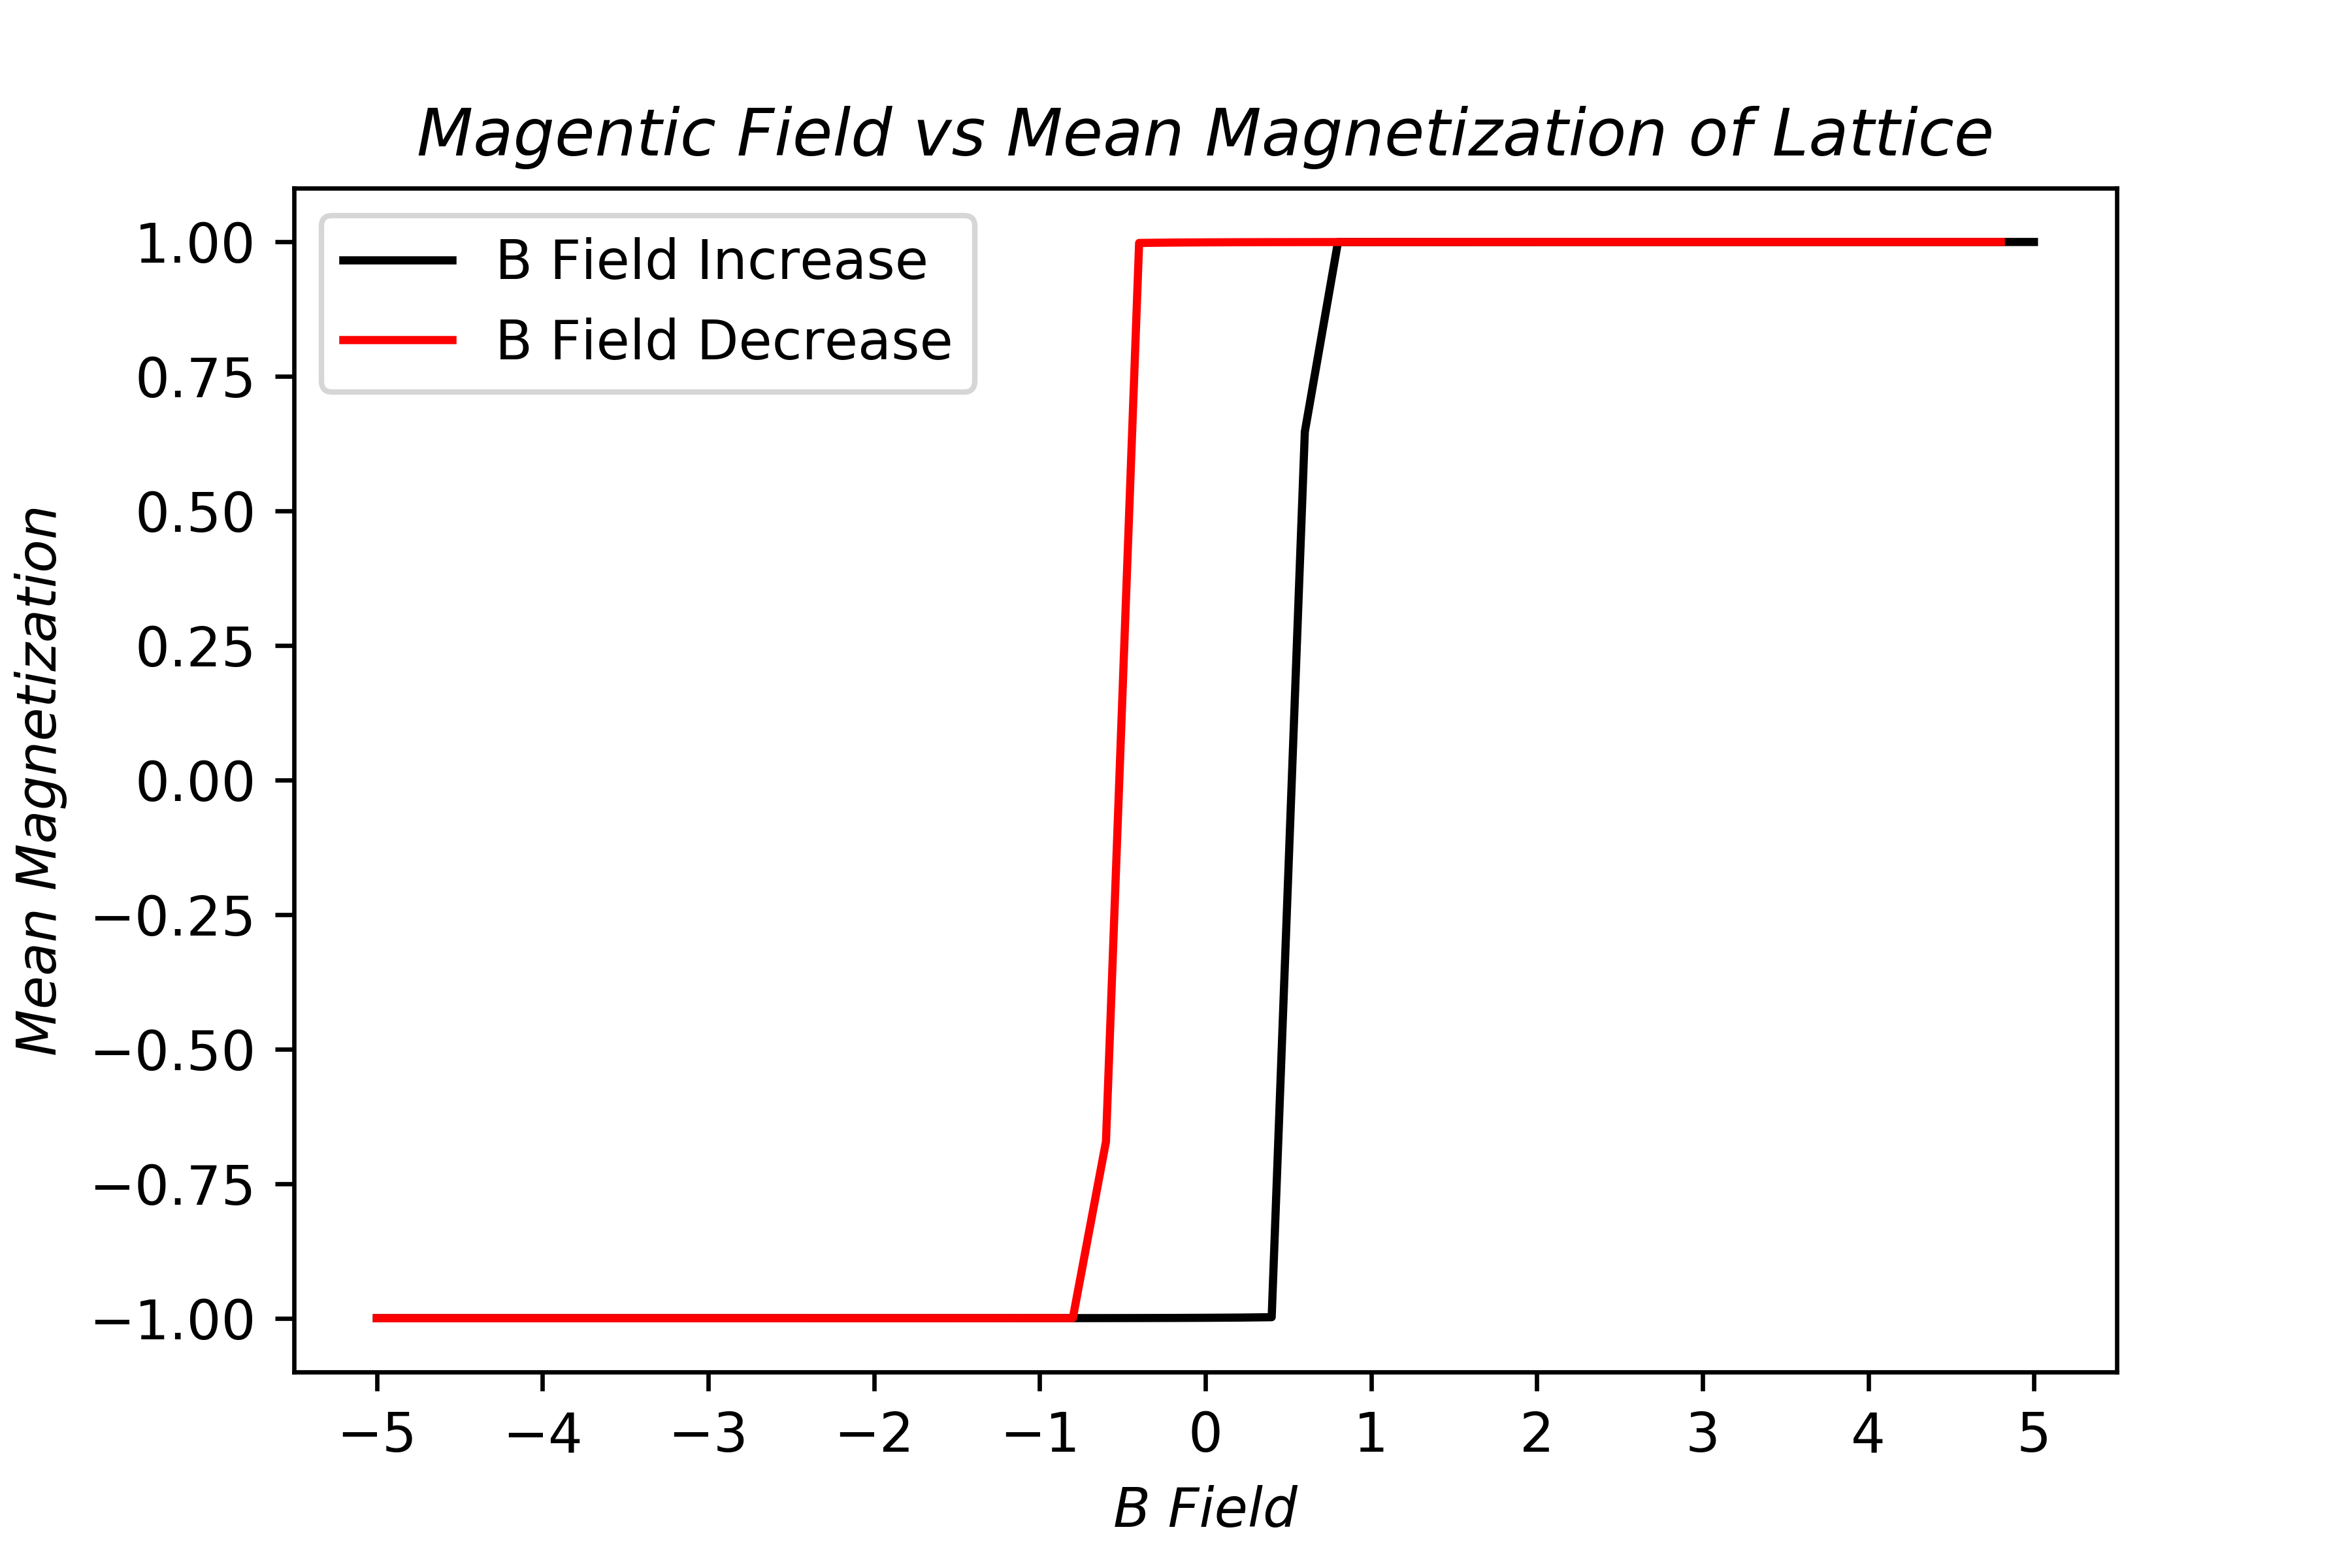
\includegraphics[scale=.5]{FirstOrderPhaseT=1Plot}
\end{figure}
\begin{figure}[h]
\caption{This plot displays the same hysteresis present in Figure 1 except in scatter plot form to show how suddenly the phase transition occurs.}
\centering
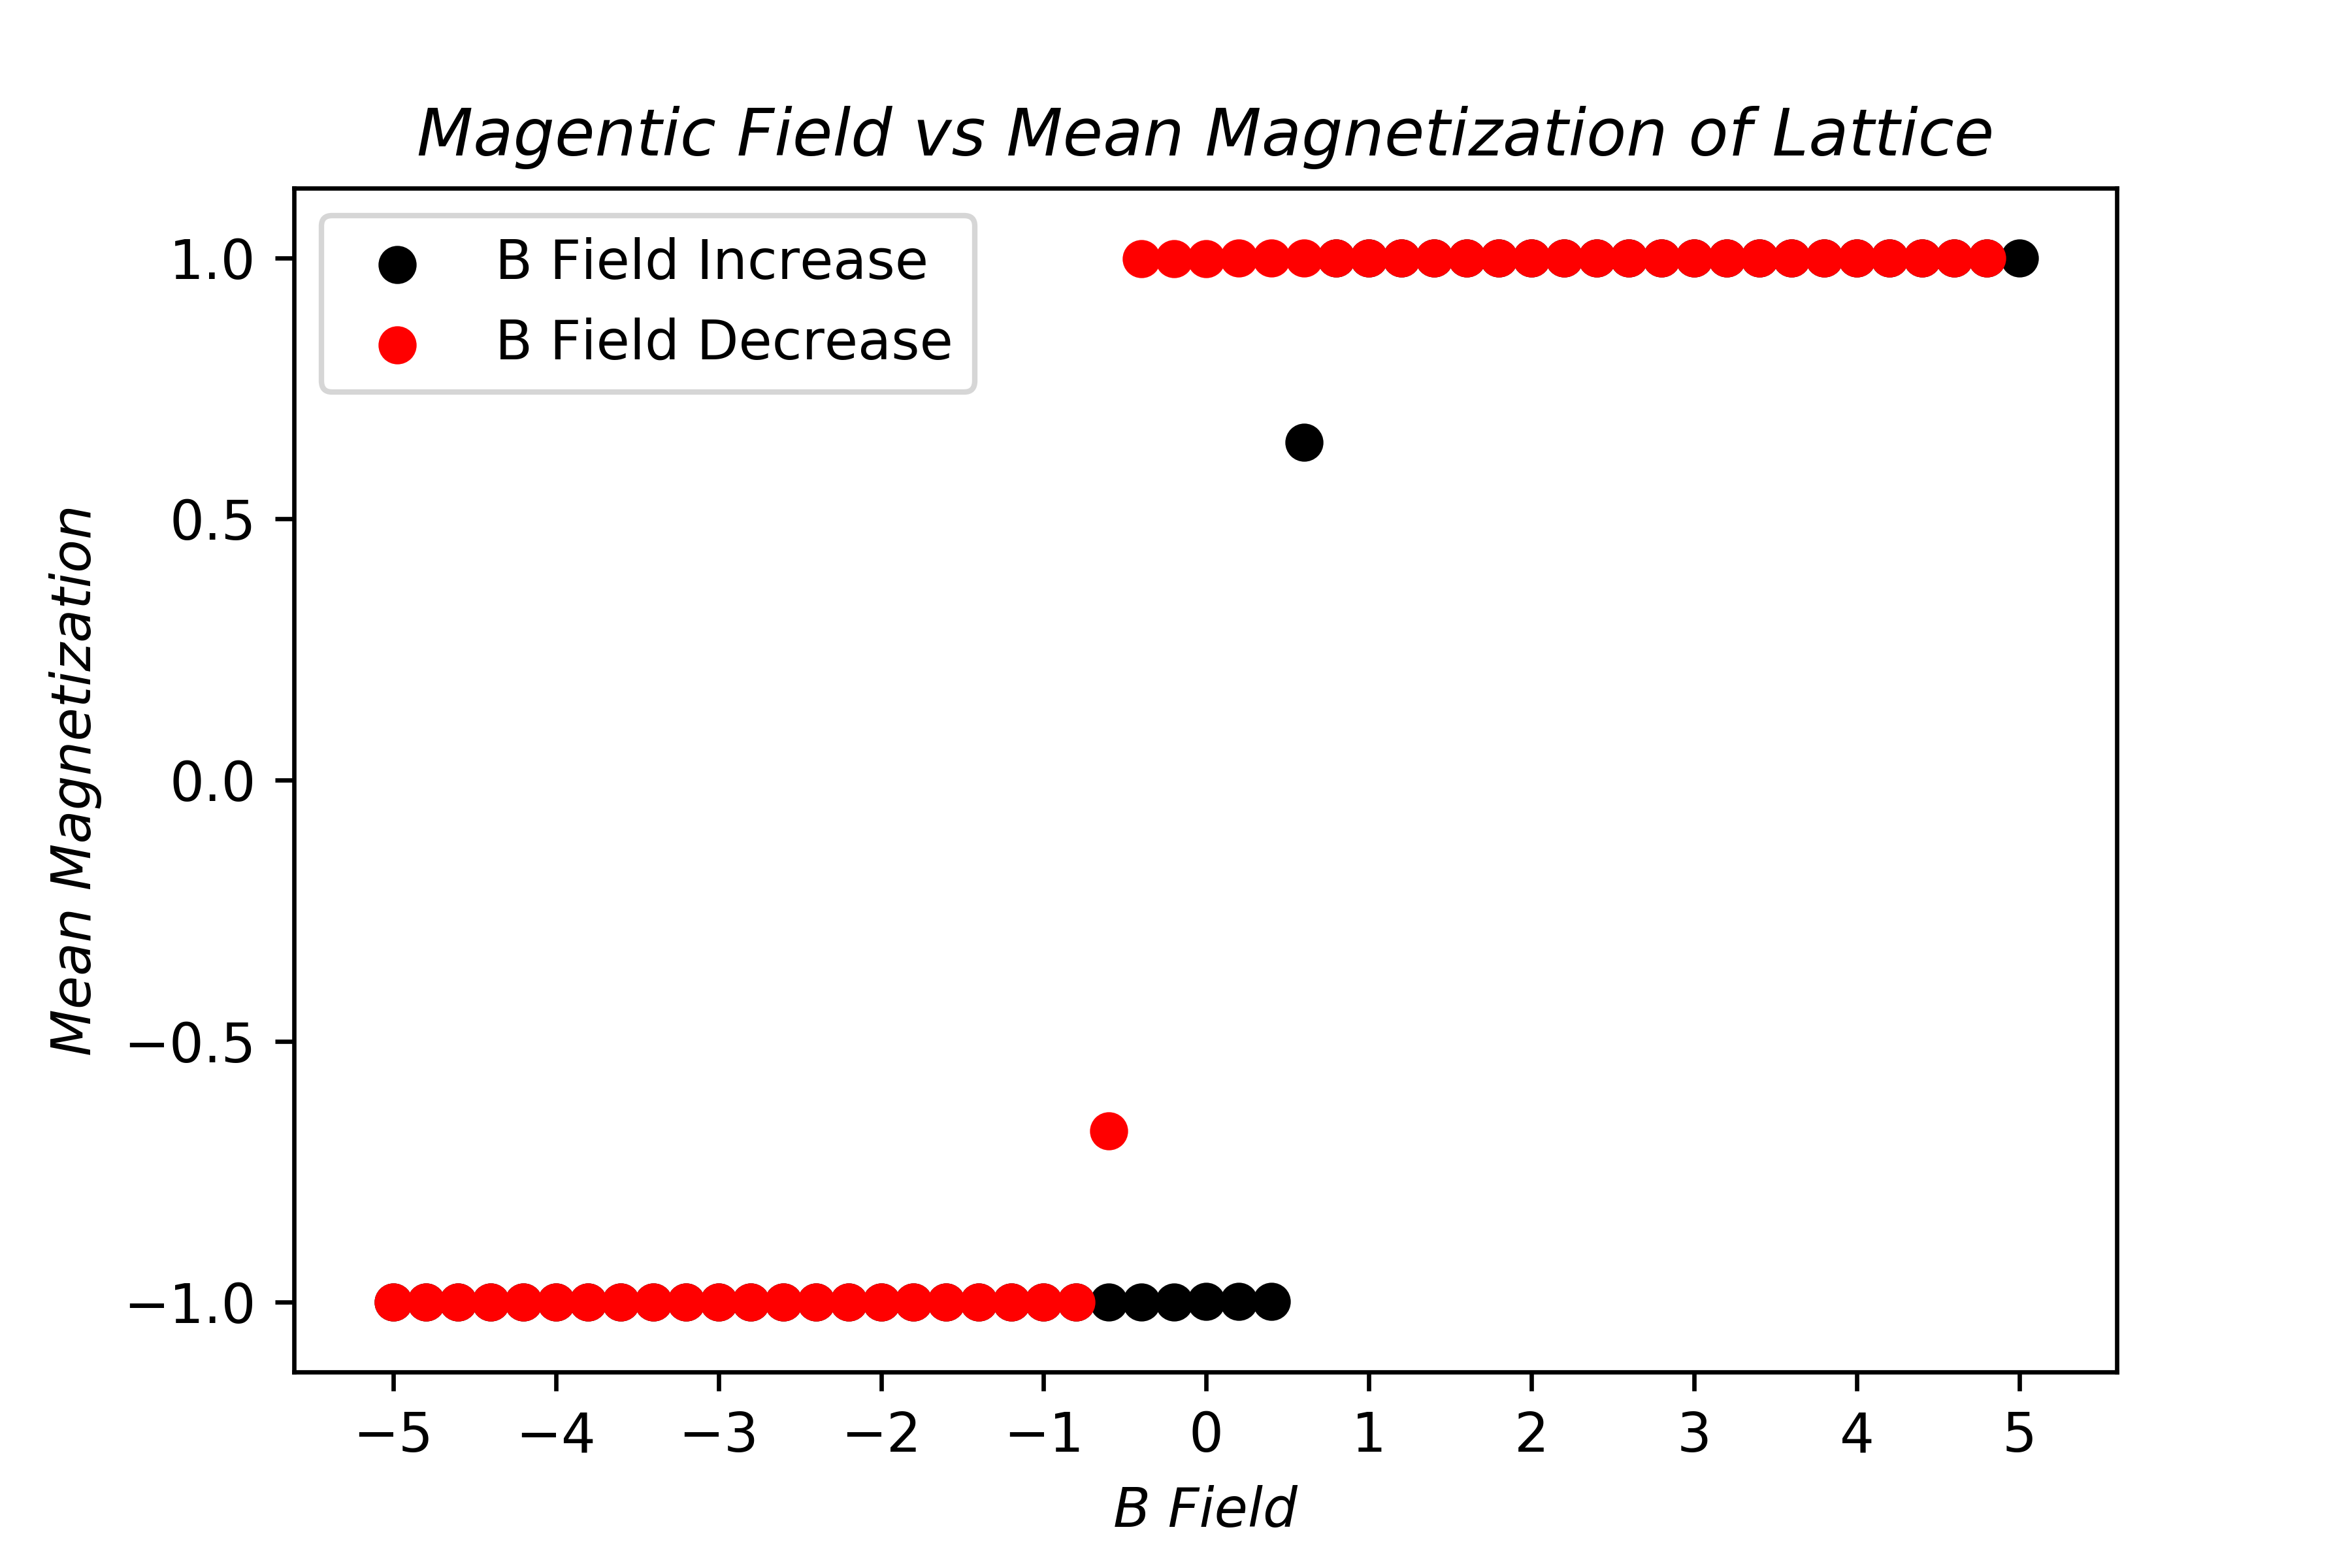
\includegraphics[scale=.5]{FirstOrderPhaseT=1Scatter}
\end{figure}
As shown in Figures (1) and (2), these discontinuities occurred very abruptly and approximately symmetrically about the $B=0$ axis creating a hysteresis. This is an important observation to make because it indicates that the lattice retains a form of "memory" as the external magnetic field of the system is altered. In other words, the former effects of the external magnetic field on the lattice cause it to react differently later on as the field is changed. Hence, this is why there exists two, rather than one, discontinuities. 

In the case that the constant temperature was $T=4 \gg T_c$, however, there existed no discontinuities within $\overline{m}$ and no hysteresis. This was a predictable observation though, because the constant temperature was greater than the critical temperature which means that no spontaneous magnetism could occur (i.e. the lattice was no longer behaving like a ferro-magnet). As shown in Figures (3) and (4), the lattice still tends towards complete alignment with the external magnetic field but it no longer has any discontinuities in $\overline{m}$ or any hysteresis. In short, when the external heat bath is at a constant temperature greater than the critical temperature, the lattice no longer retains a "memory" like it did in the case that the constant temperature was less than the critical temperature. 
\begin{figure}[H]
\caption{This plot displays the Ising model lattice when $T=4$ across the domain of all the magnetic field increments. Here there exists no hysteresis.}
\centering
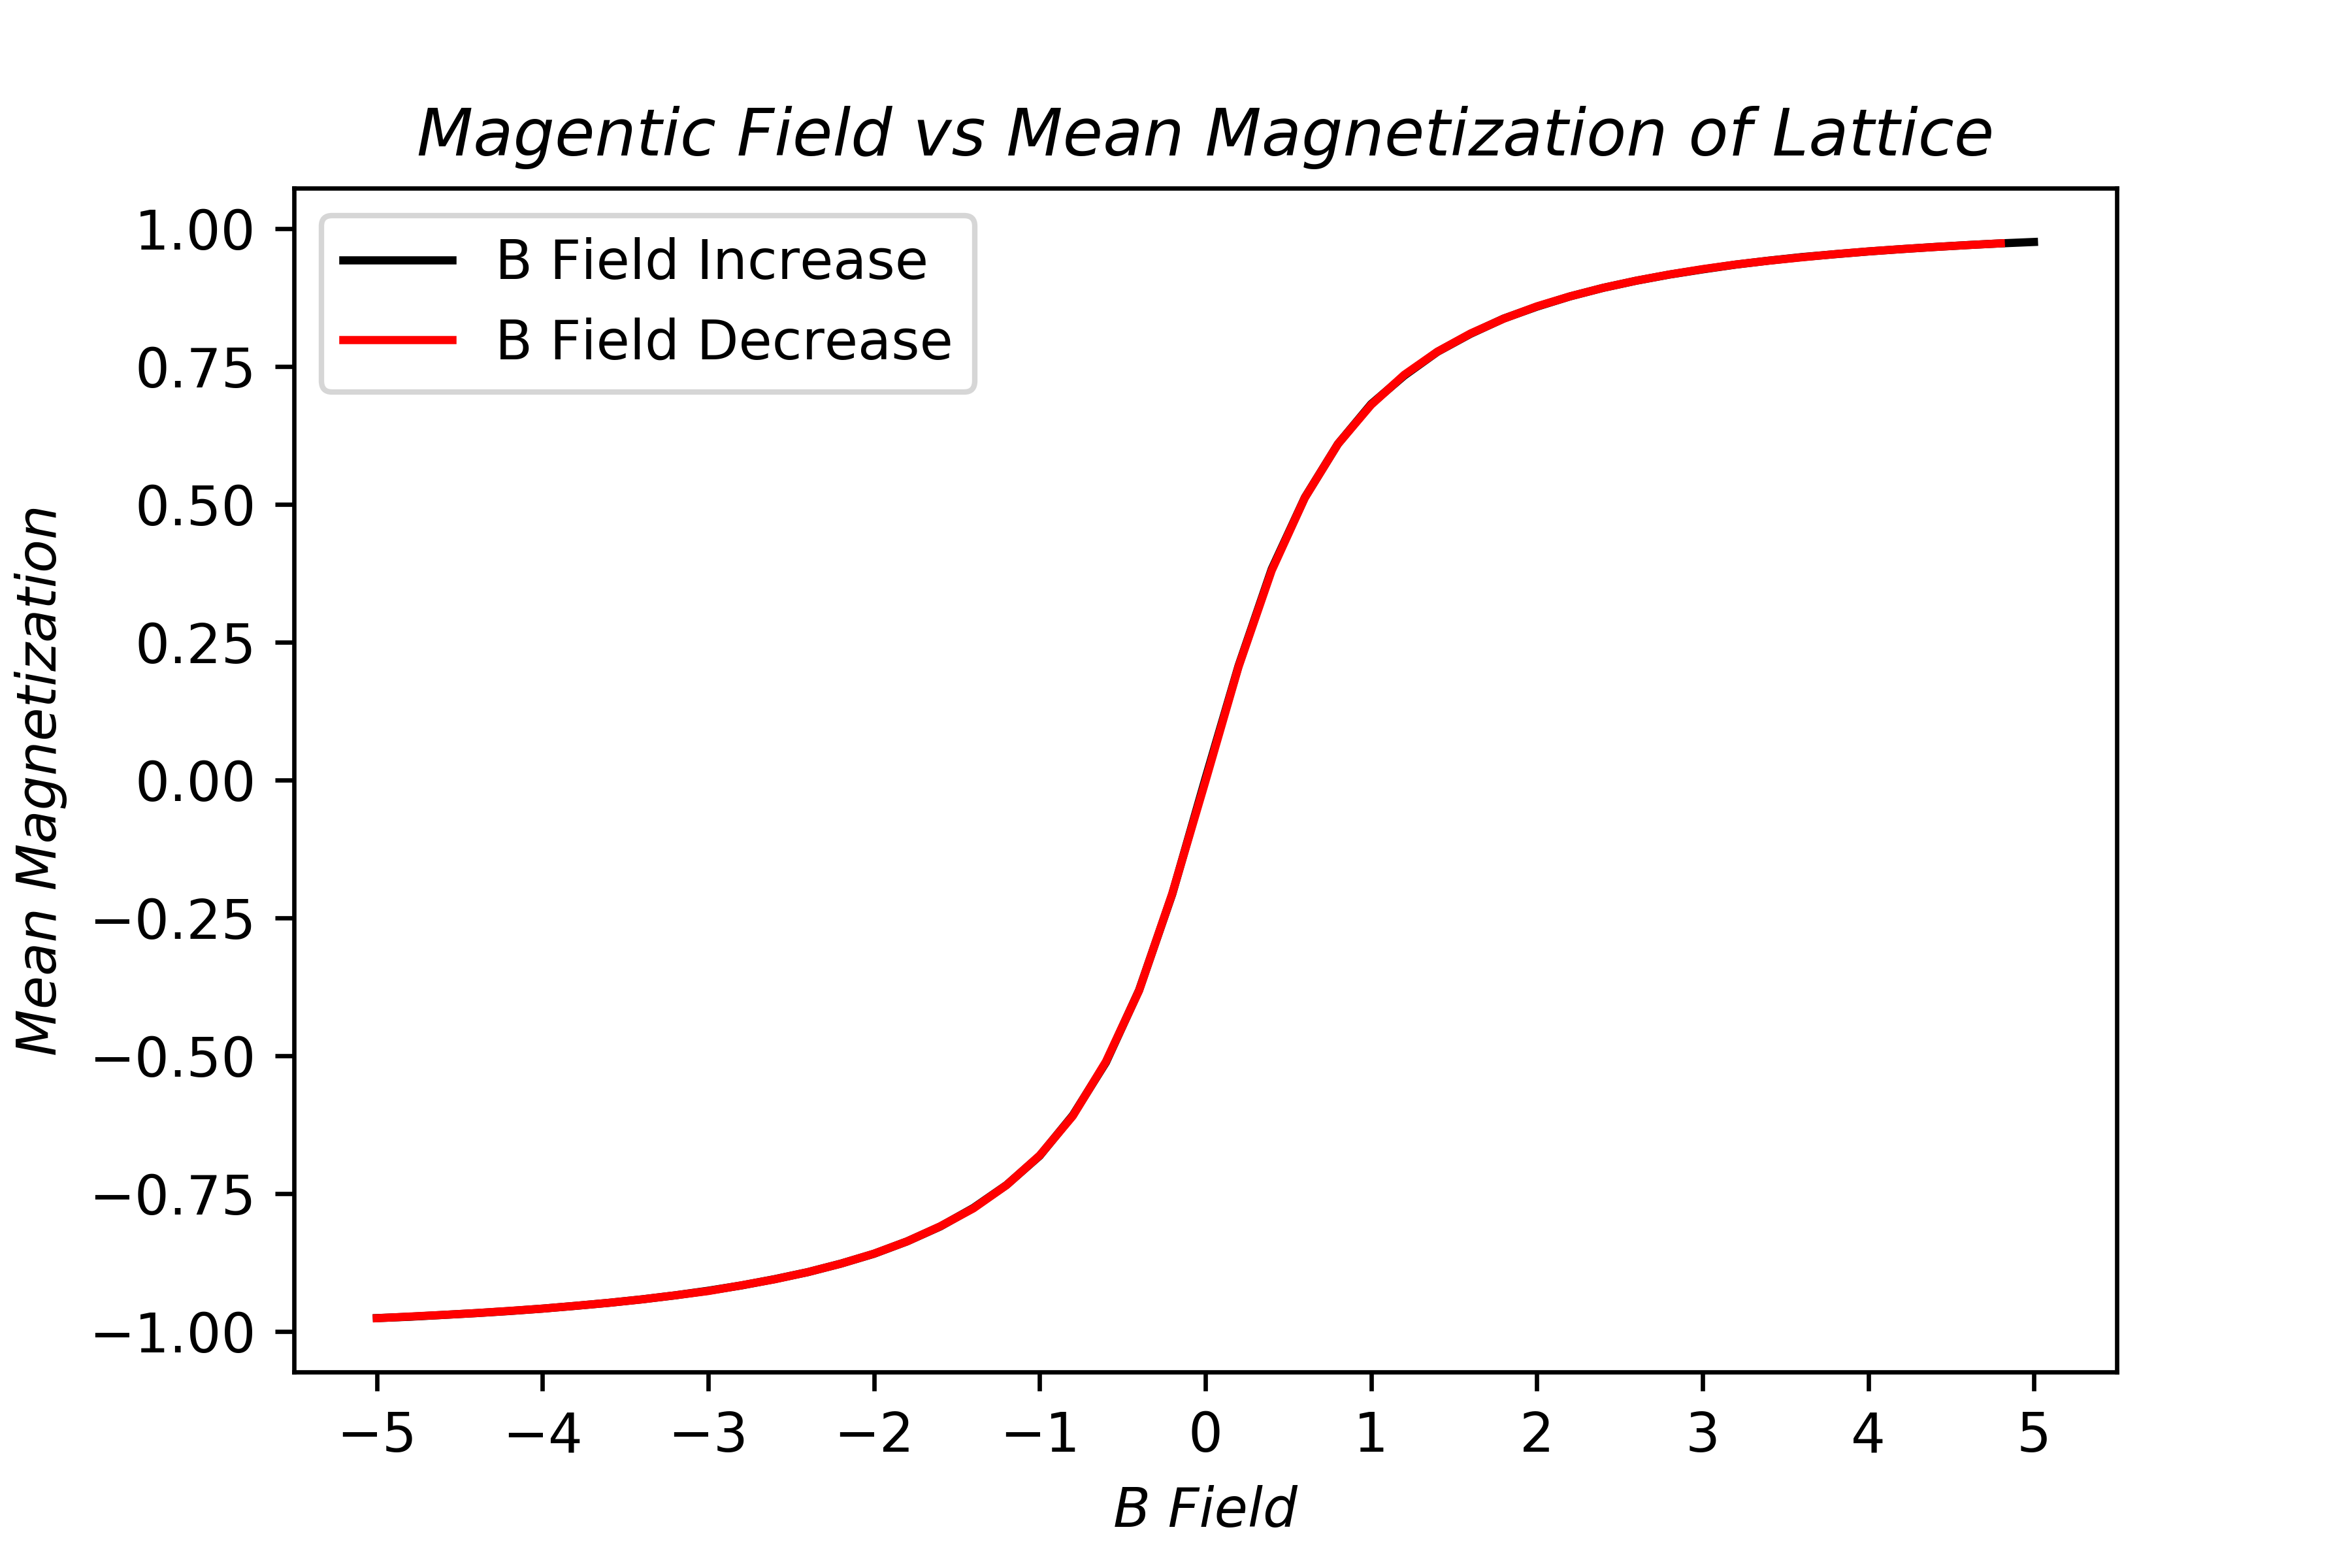
\includegraphics[scale=.5]{FirstOrderPhaseT=4Plot}
%\end{figure}
%\begin{figure}[h]
\caption{This plot displays the same information present in Figure 3 except in scatter plot form, to show how quick changes in $\overline{m}$ occurred.}
\centering
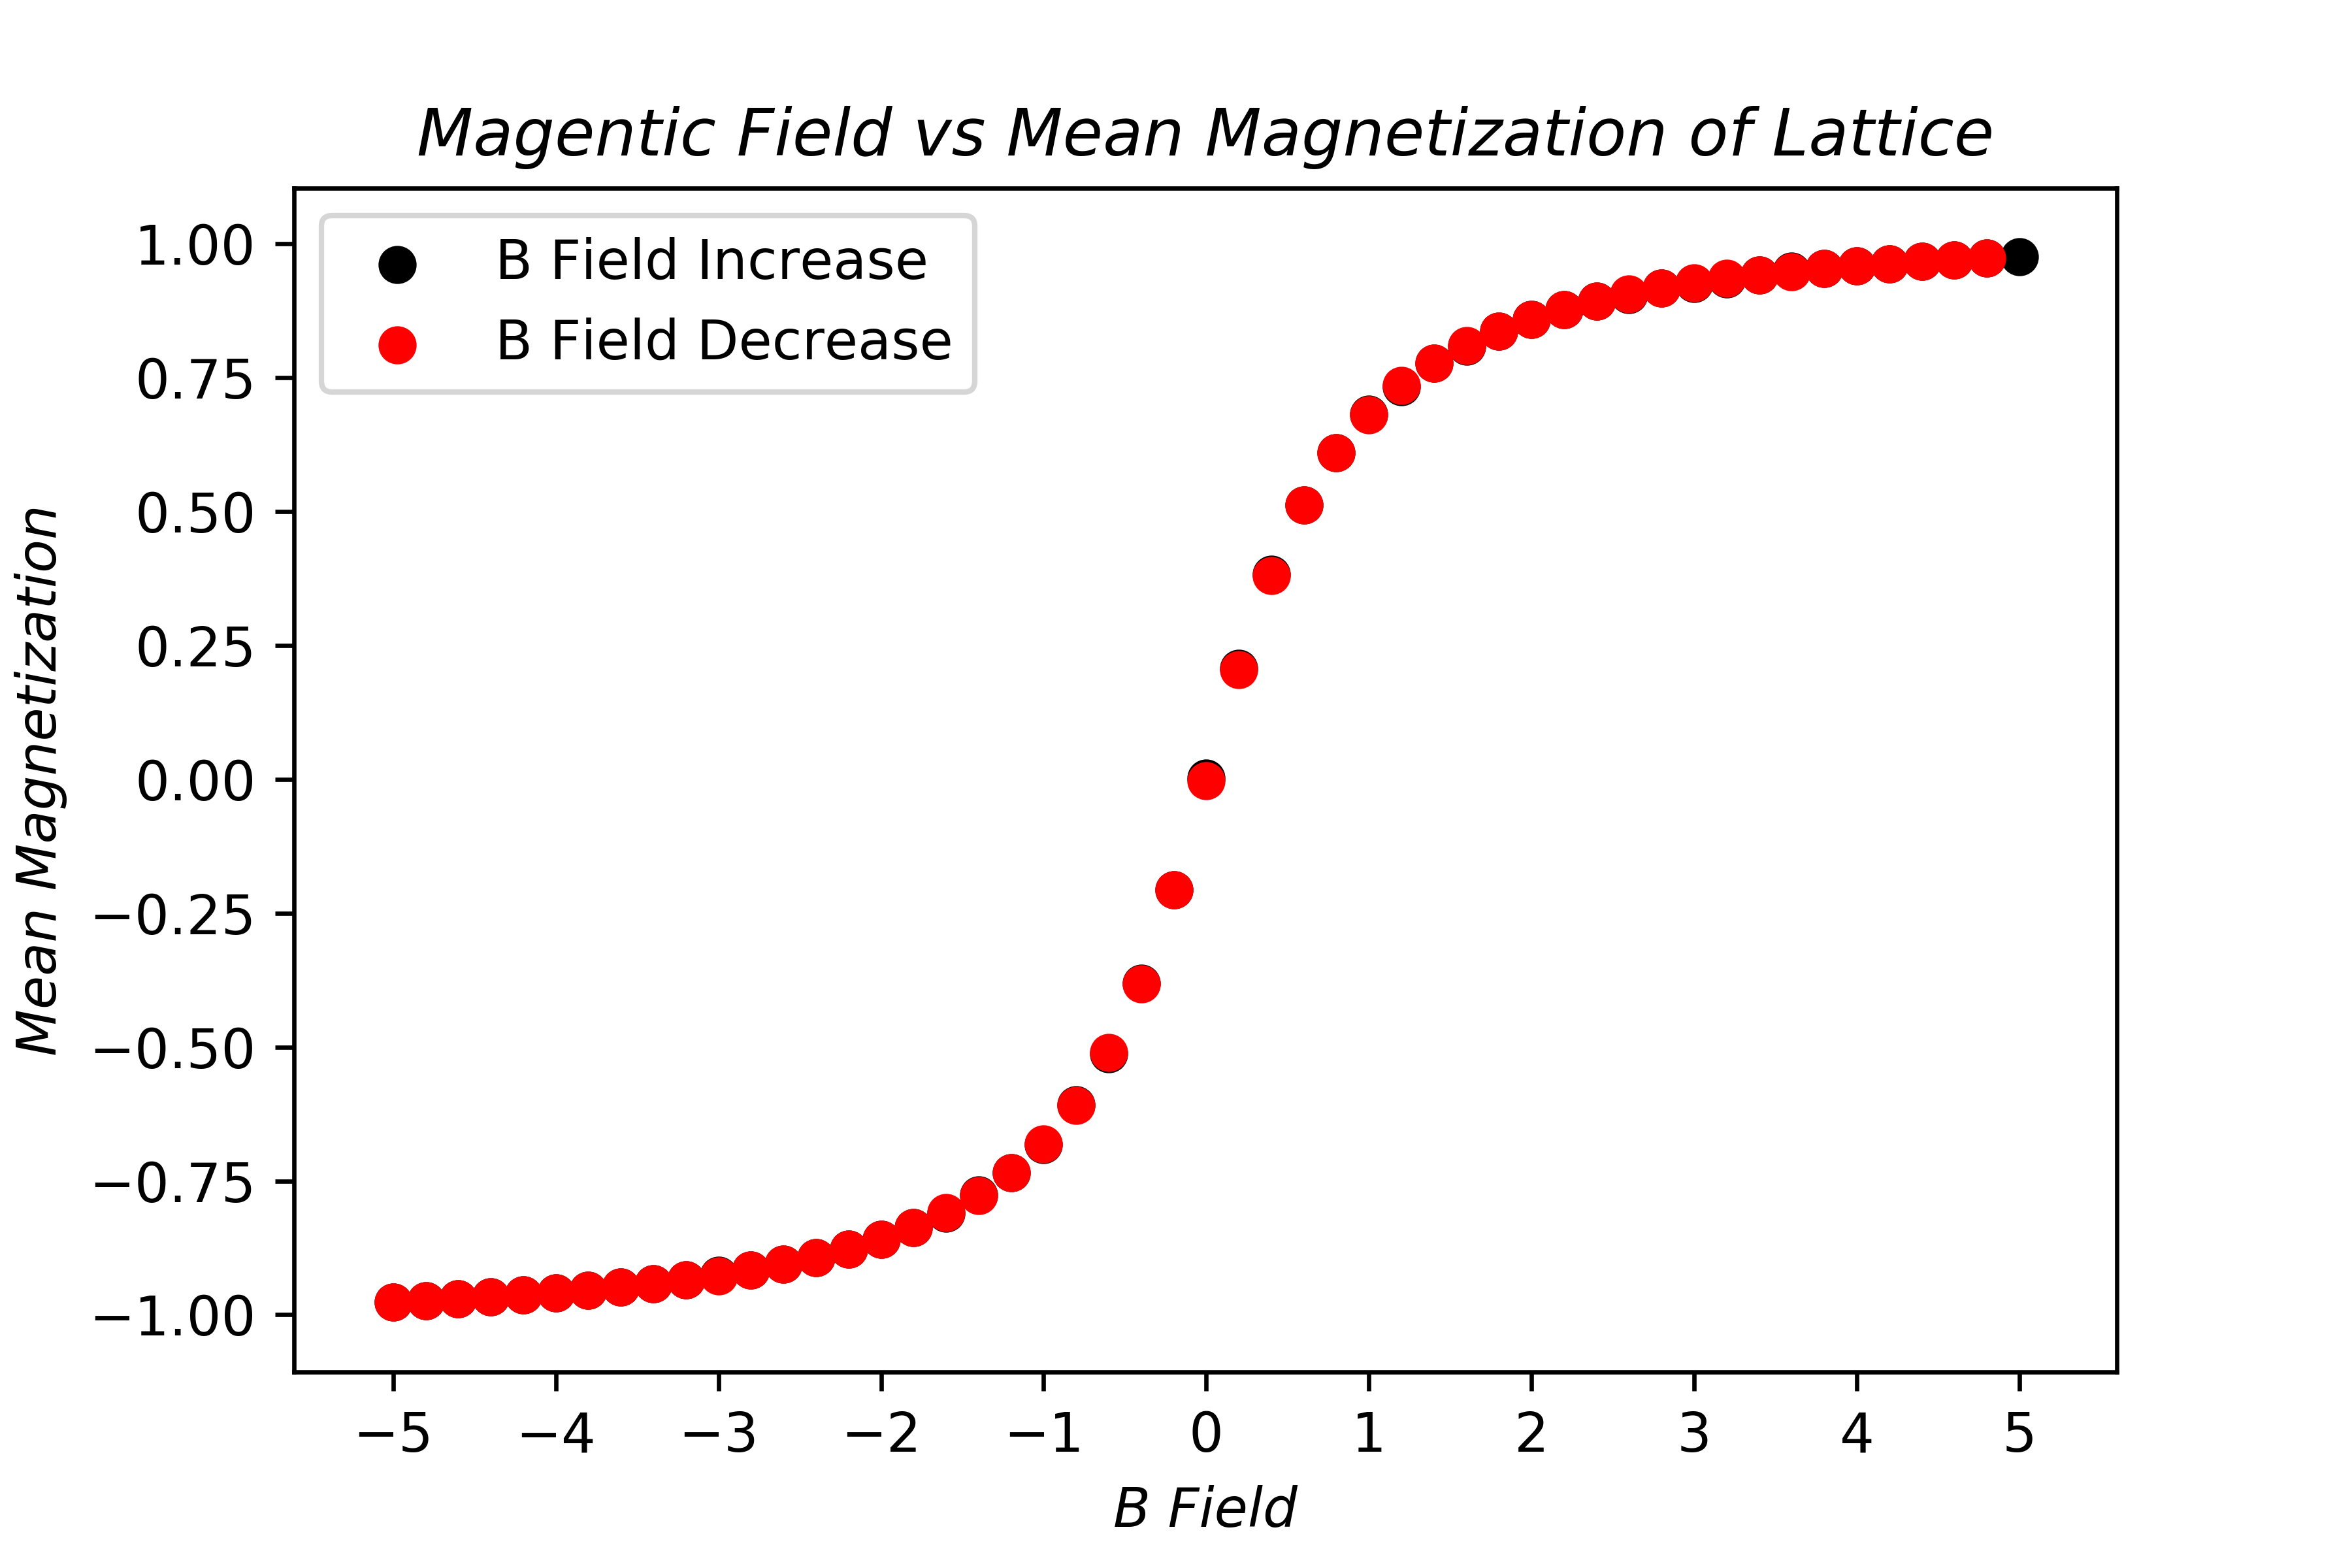
\includegraphics[scale=.5]{FirstOrderPhaseT=4Scatter}
\end{figure} 
Part two of the first experiment sought to determine whether or not the number of independent samples was dependent or not on the magnitude of the magnetic field and to use a conservative estimate to add error bars to the values of $\overline{m}$. In regards to the number of independent samples, this quantity was calculated by searching for the number of distinct structures within the plotted auto-correlation function outlined in equation (4). This analysis revealed that the number of independent samples certainly does rely on the relationship between the magnetic field and the heat bath. For the cases $T \ll B$ and $T \approx B$, the plotted auto-correlation function discerned similar structures that largely fluctuated about 0 until the latter quarter of the samples, which was expected as there is less information for the auto-correlation to compare to the further down the signal it goes. Using a conservative estimate for the number of independent samples, there appeared to be $\approx40$ independent structures for $T \ll B$ which can be seen in Figure (5), and $\approx 25$ independent structures for $T \approx B$ which can be seen in Figure (6).
\begin{figure}[H]
\caption{This plot displays auto-correlation of $\overline{m}$ in the case that $T \ll B$. The structure fluctuates quite a bit especially in the latter sections. In total there approximately 40 independent structures.}
\centering
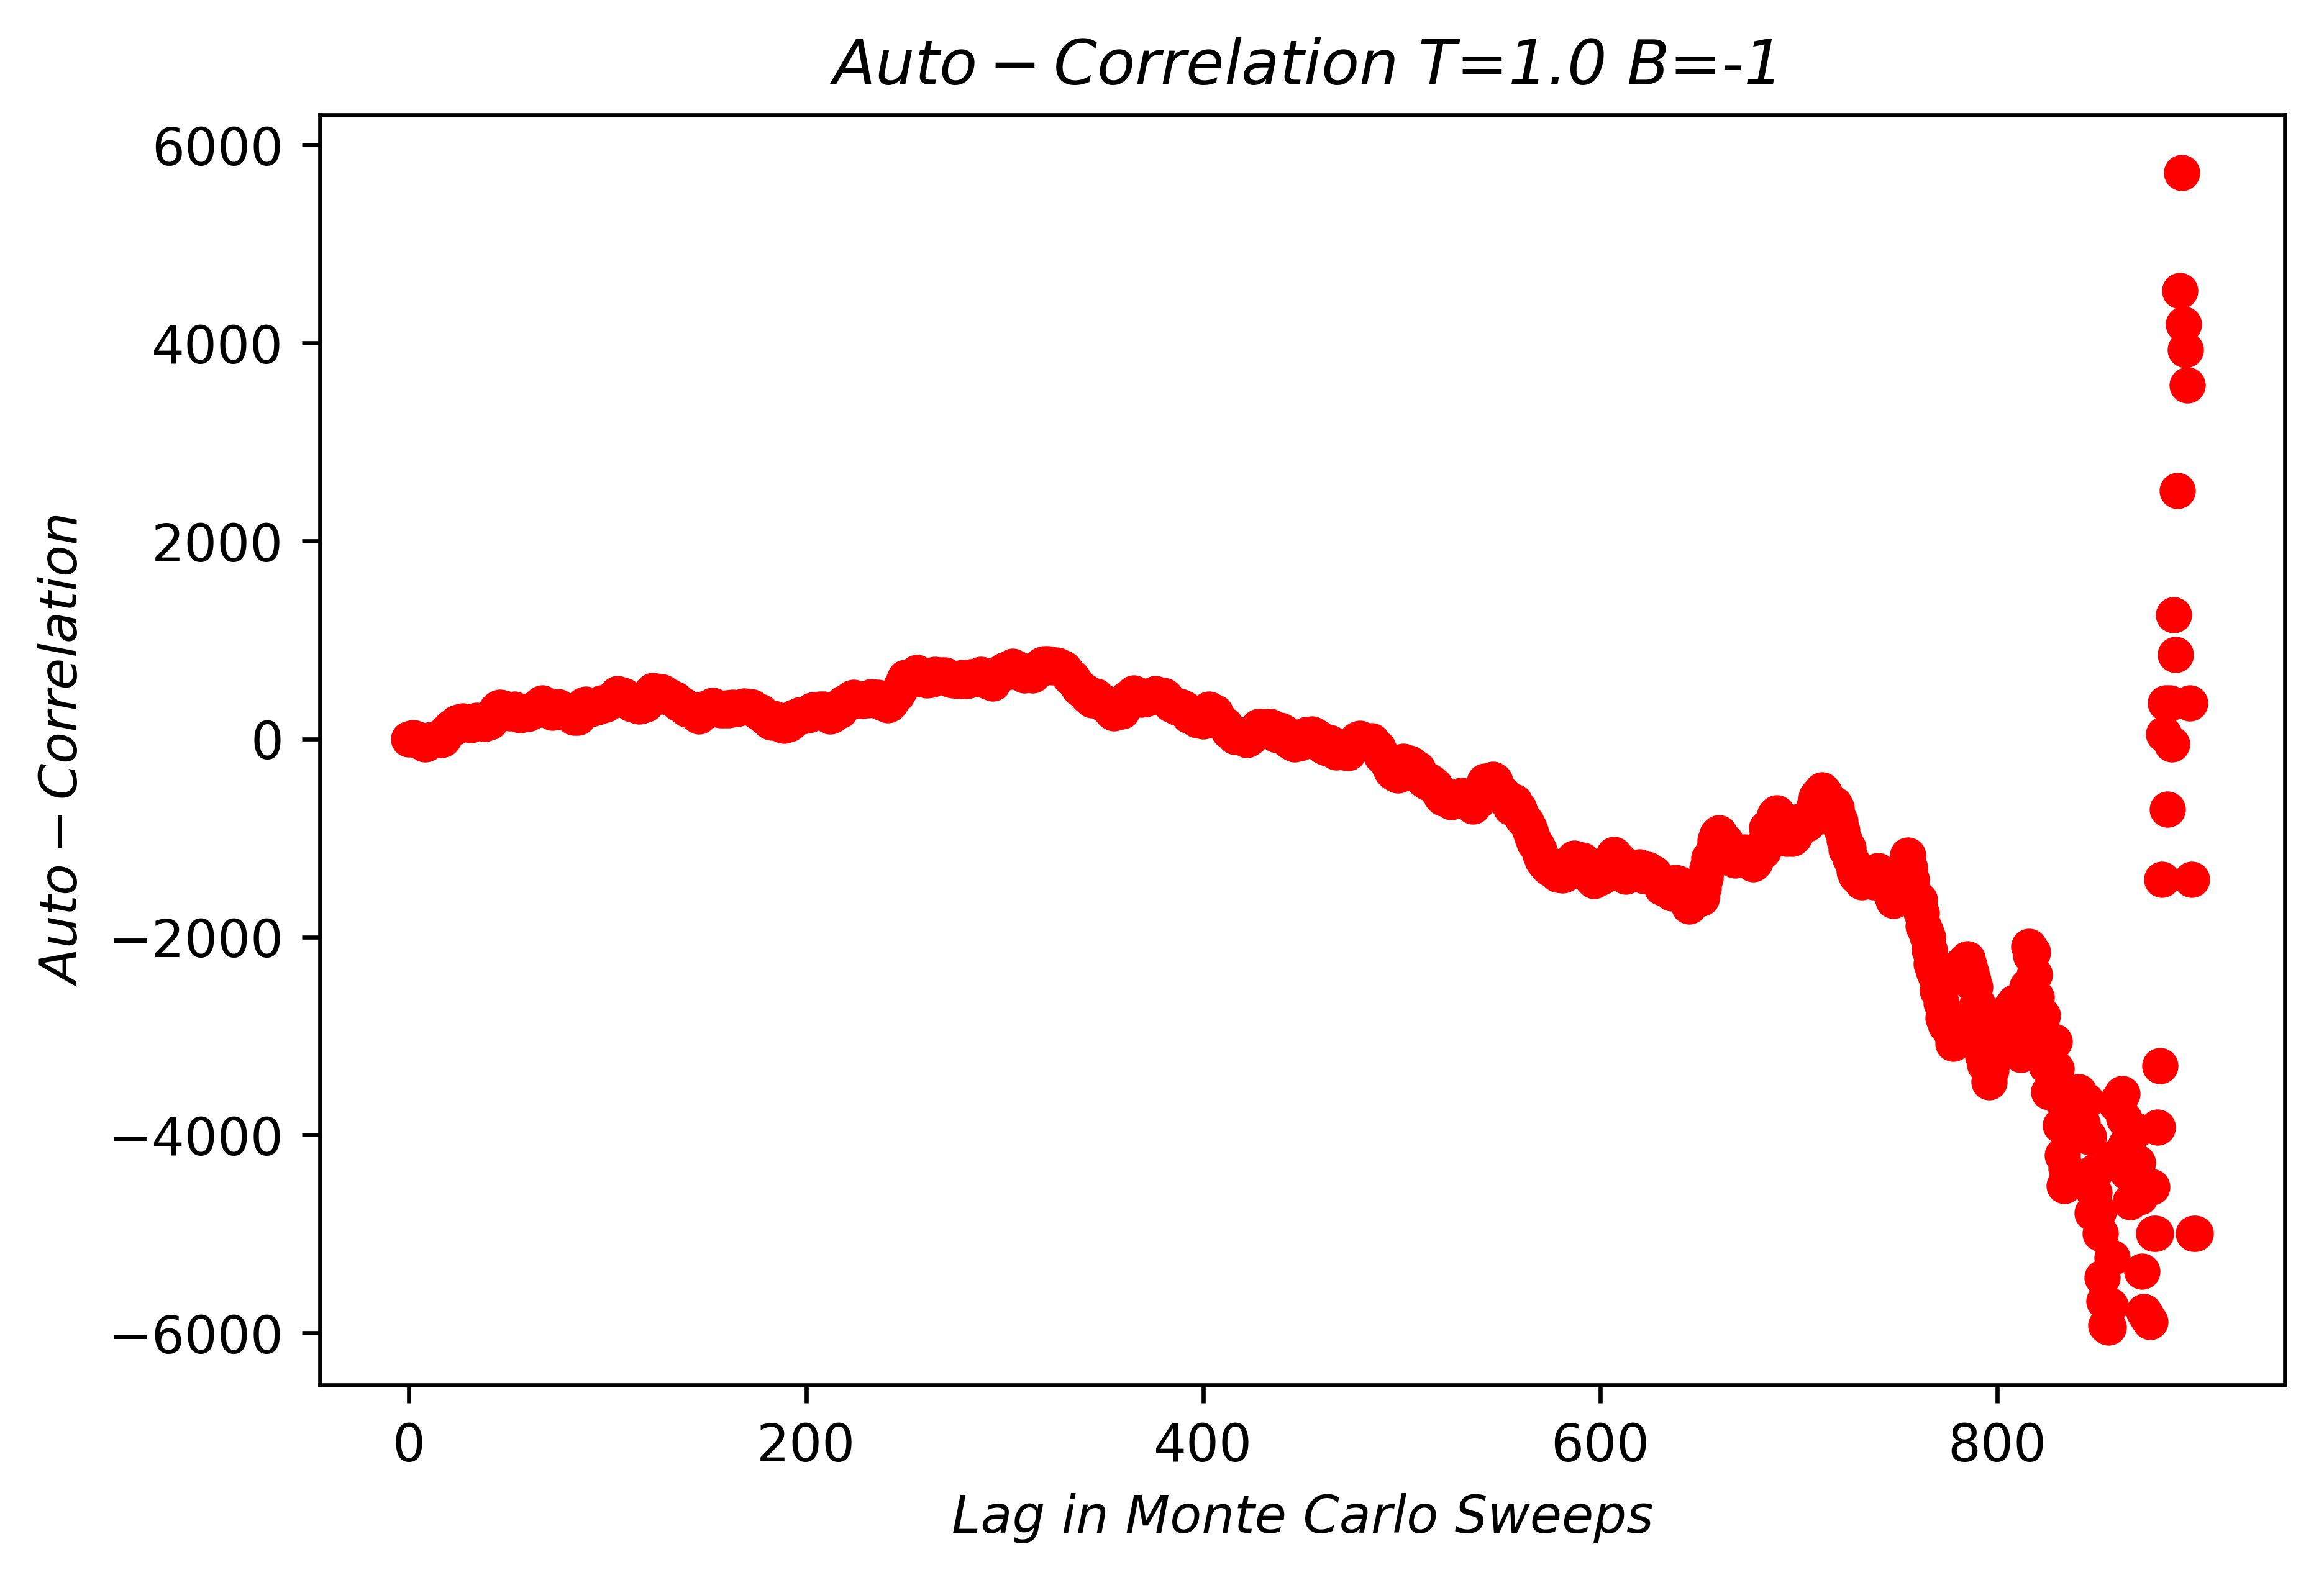
\includegraphics[scale=.5]{AutocorrelationT=1B=minus1Scatter}
\end{figure}
\begin{figure}[h]
\caption{This plot displays auto-correlation of $\overline{m}$ in the case that $T \approx B$. The structure fluctuates quite a bit especially in the latter sections like Figure (5). In total there approximately 25 independent structures.}
\centering
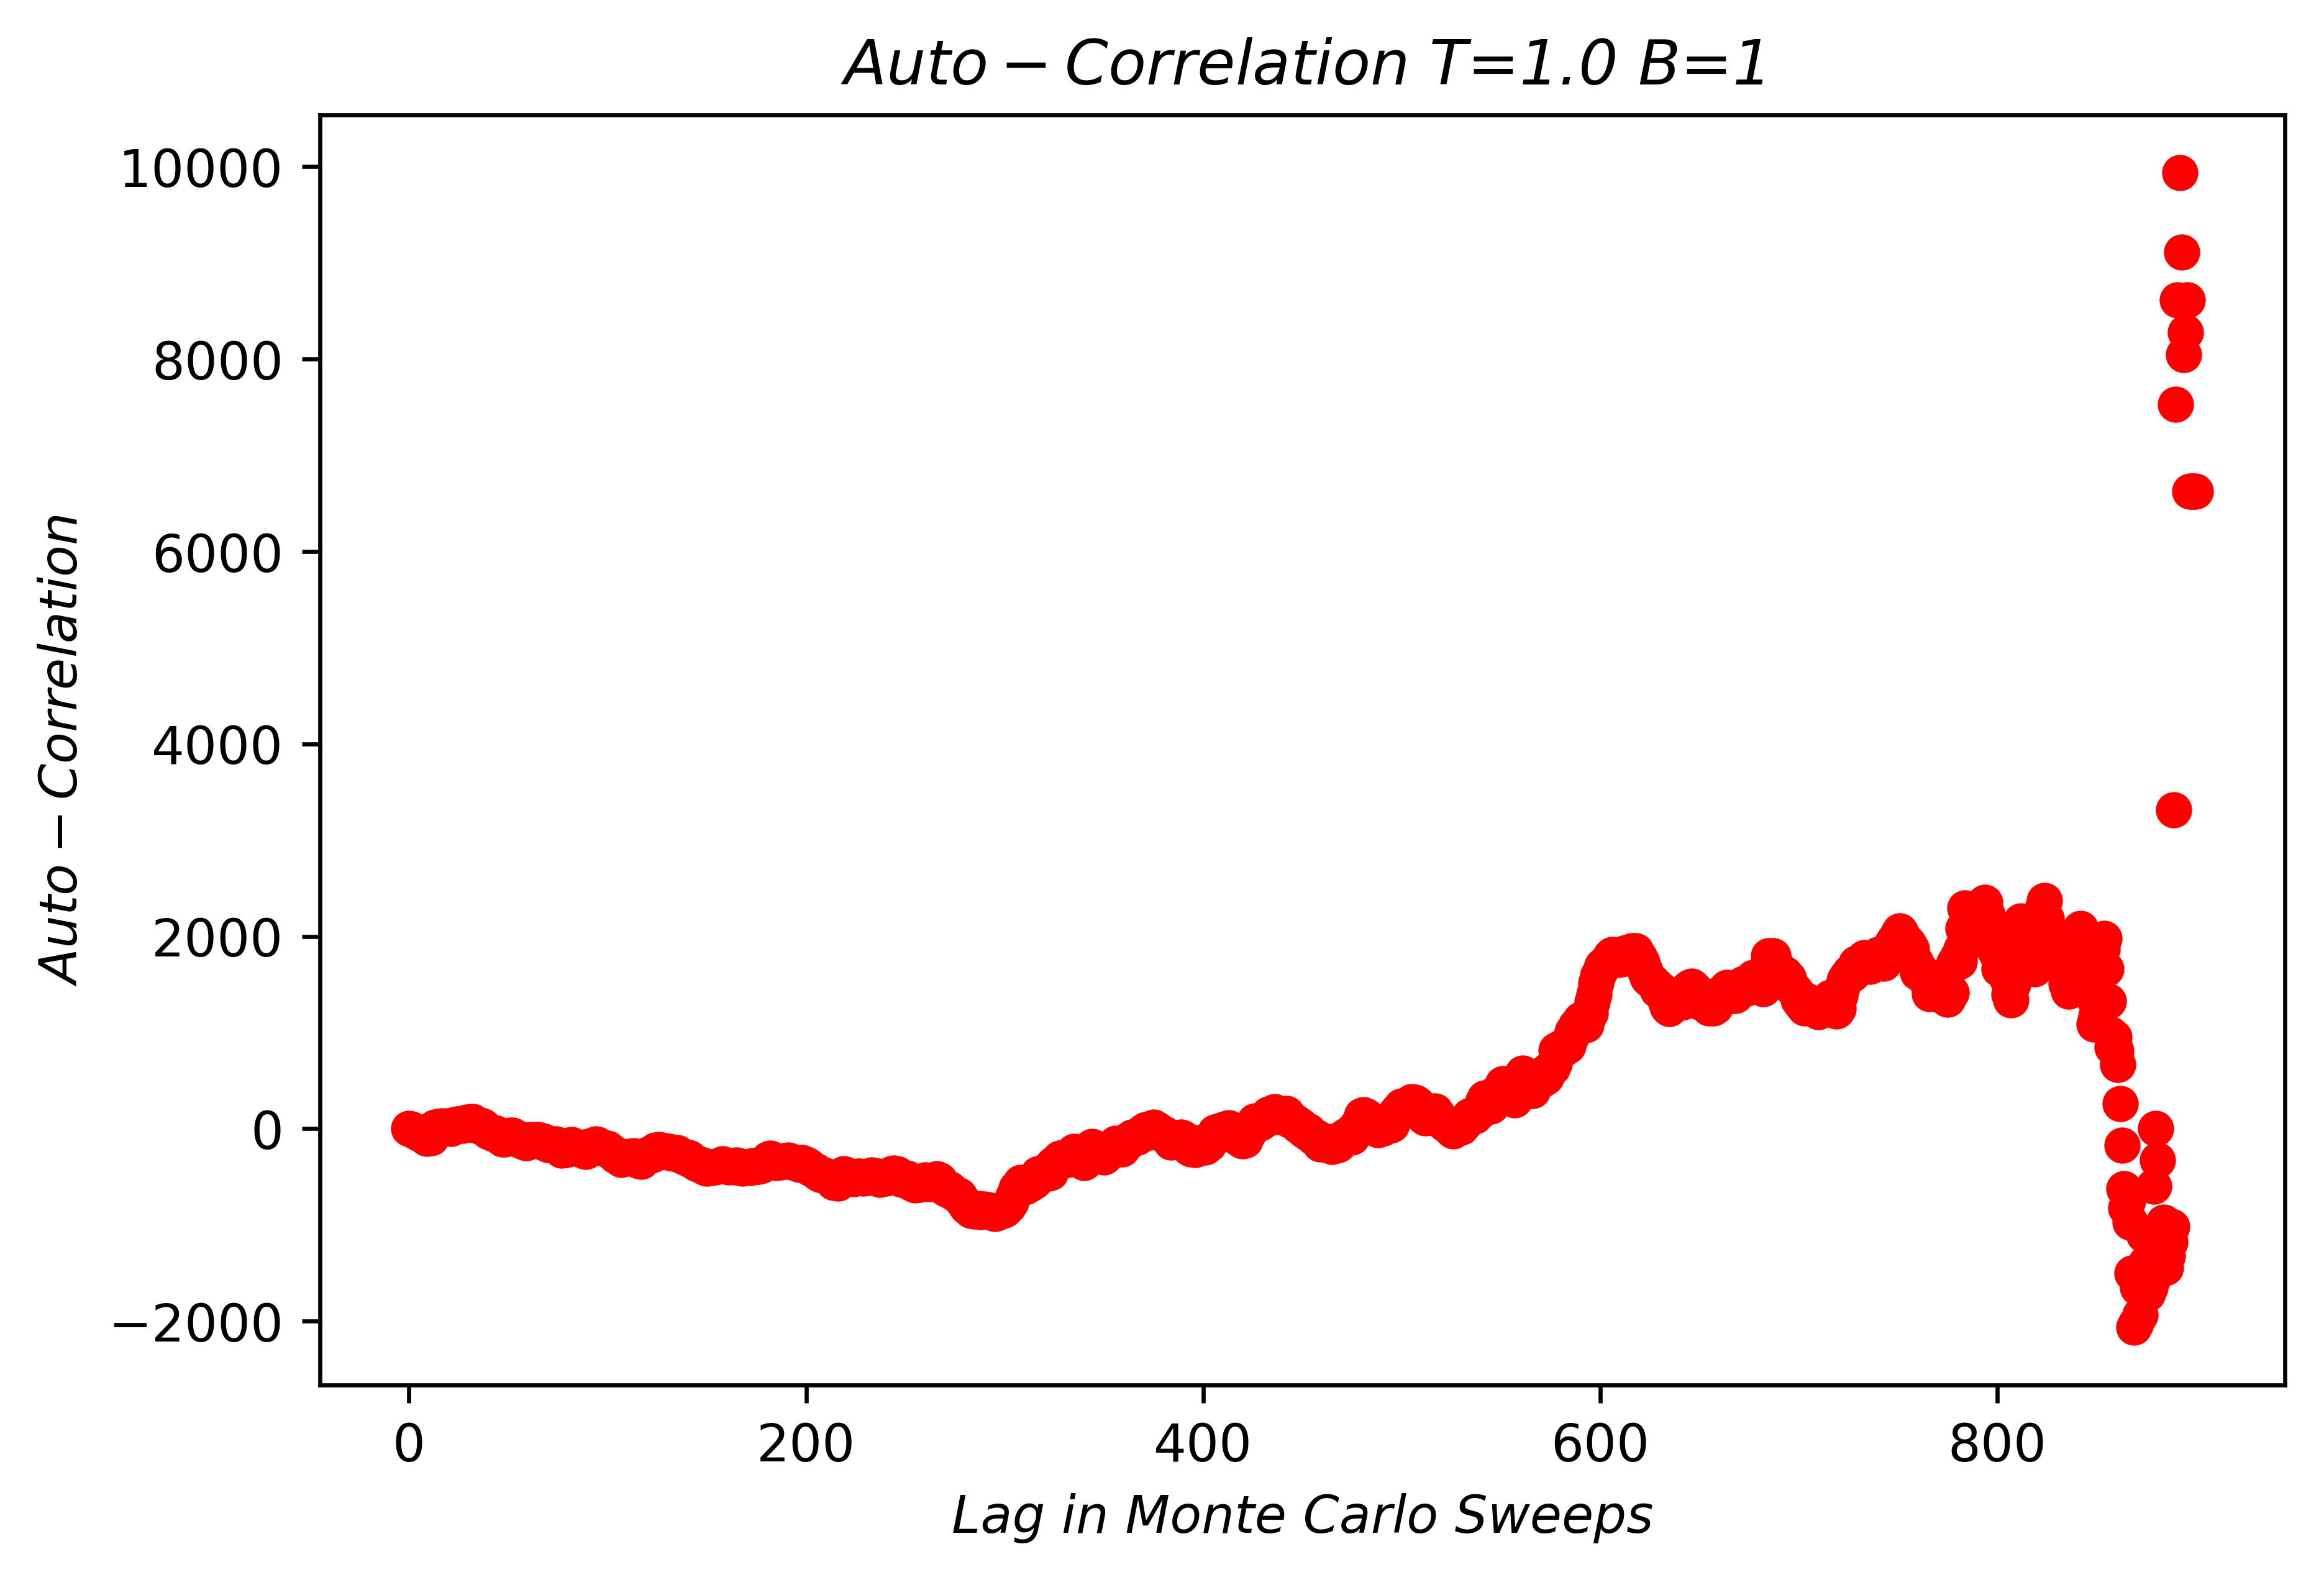
\includegraphics[scale=.5]{AutocorrelationT=1B=1Scatter}
\end{figure} 
\hspace{-3.8mm}In the case that $T \gg B$, however, the structure of the auto-correlation plot was much more distinct and can easily be discerned to have exactly 23 structures or in other words, 23 independent samples, which can be seen in Figure (7).\\
\begin{figure}[H]
\caption{This plot displays auto-correlation of $\overline{m}$ in the case that $T \gg B$. The structure fluctuates quite a bit especially in the latter sections like Figure (5). In total there are exactly 23 independent structures.}
\centering
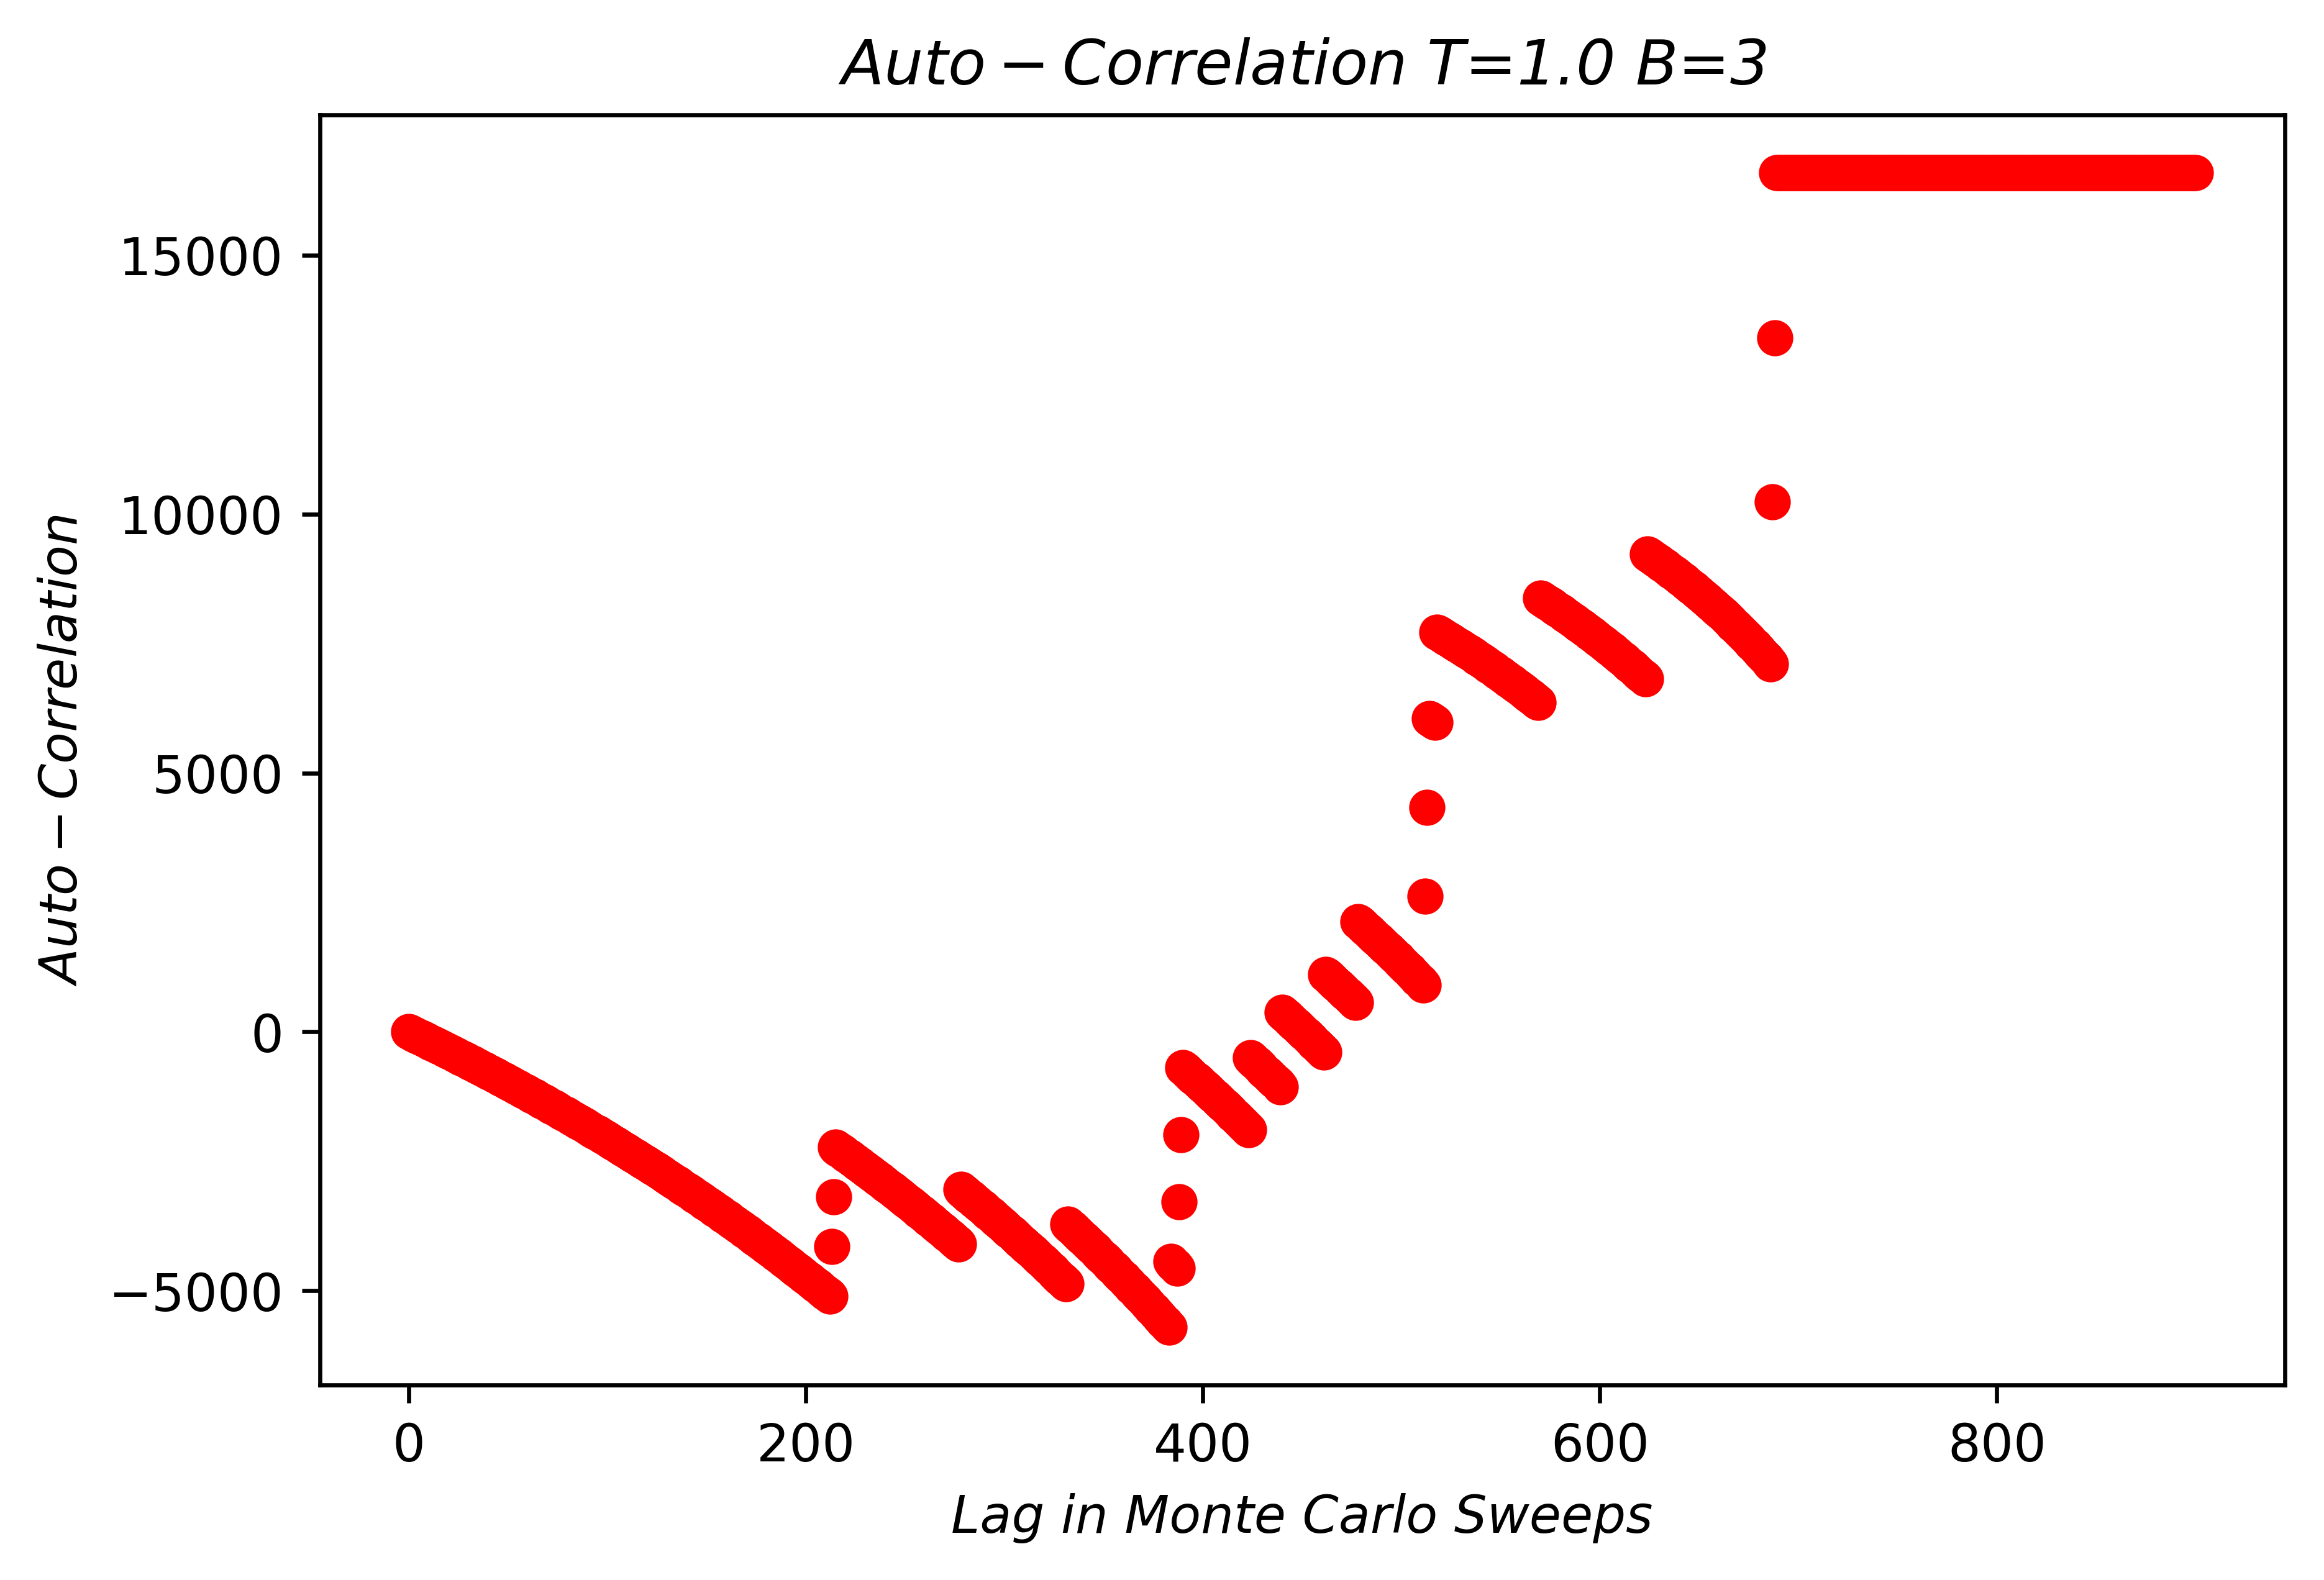
\includegraphics[scale=.5]{AutocorrelationT=1B=3Scatter}
\end{figure}
\hspace{-3.8mm}In order to add error bars to the values of $\overline{m}$ the standard deviation had to be applied to upper and lower bounds of $\overline{m}$. The standard deviation was acquired by using the same 900 non-discarded Monte-Carlo sweeps as in part one of the experiment and turned out to be: 0.000105 in the case that $T \ll B$, .000104 in the case that $T \approx B$, and 5.744 in the case that $T \gg B$. Clearly, the error bars for the case $T \gg B$ are significantly larger than the other two, and hence, has the largest room for error in its auto-correlation calculations.
%%%%%%%%%%%%%%%%%%%%%%%%%%%%%%%%%%%
% New Section
%%%%%%%%%%%%%%%%%%%%%%%%%%%%%%%%%%%
\begin{figure}[H]
\caption{This plot shows the evolution of $\overline{m}$ for a randomly aligned lattice in the case that $T=1 \ll T_c$. The evolution appears to be split into three distinct periods: prior to 500, $\overline{m}$ trends deeply downwards, before coming to a more consistent decrease, and finally plateauing around 1750 when thermalization occurs.}
\centering
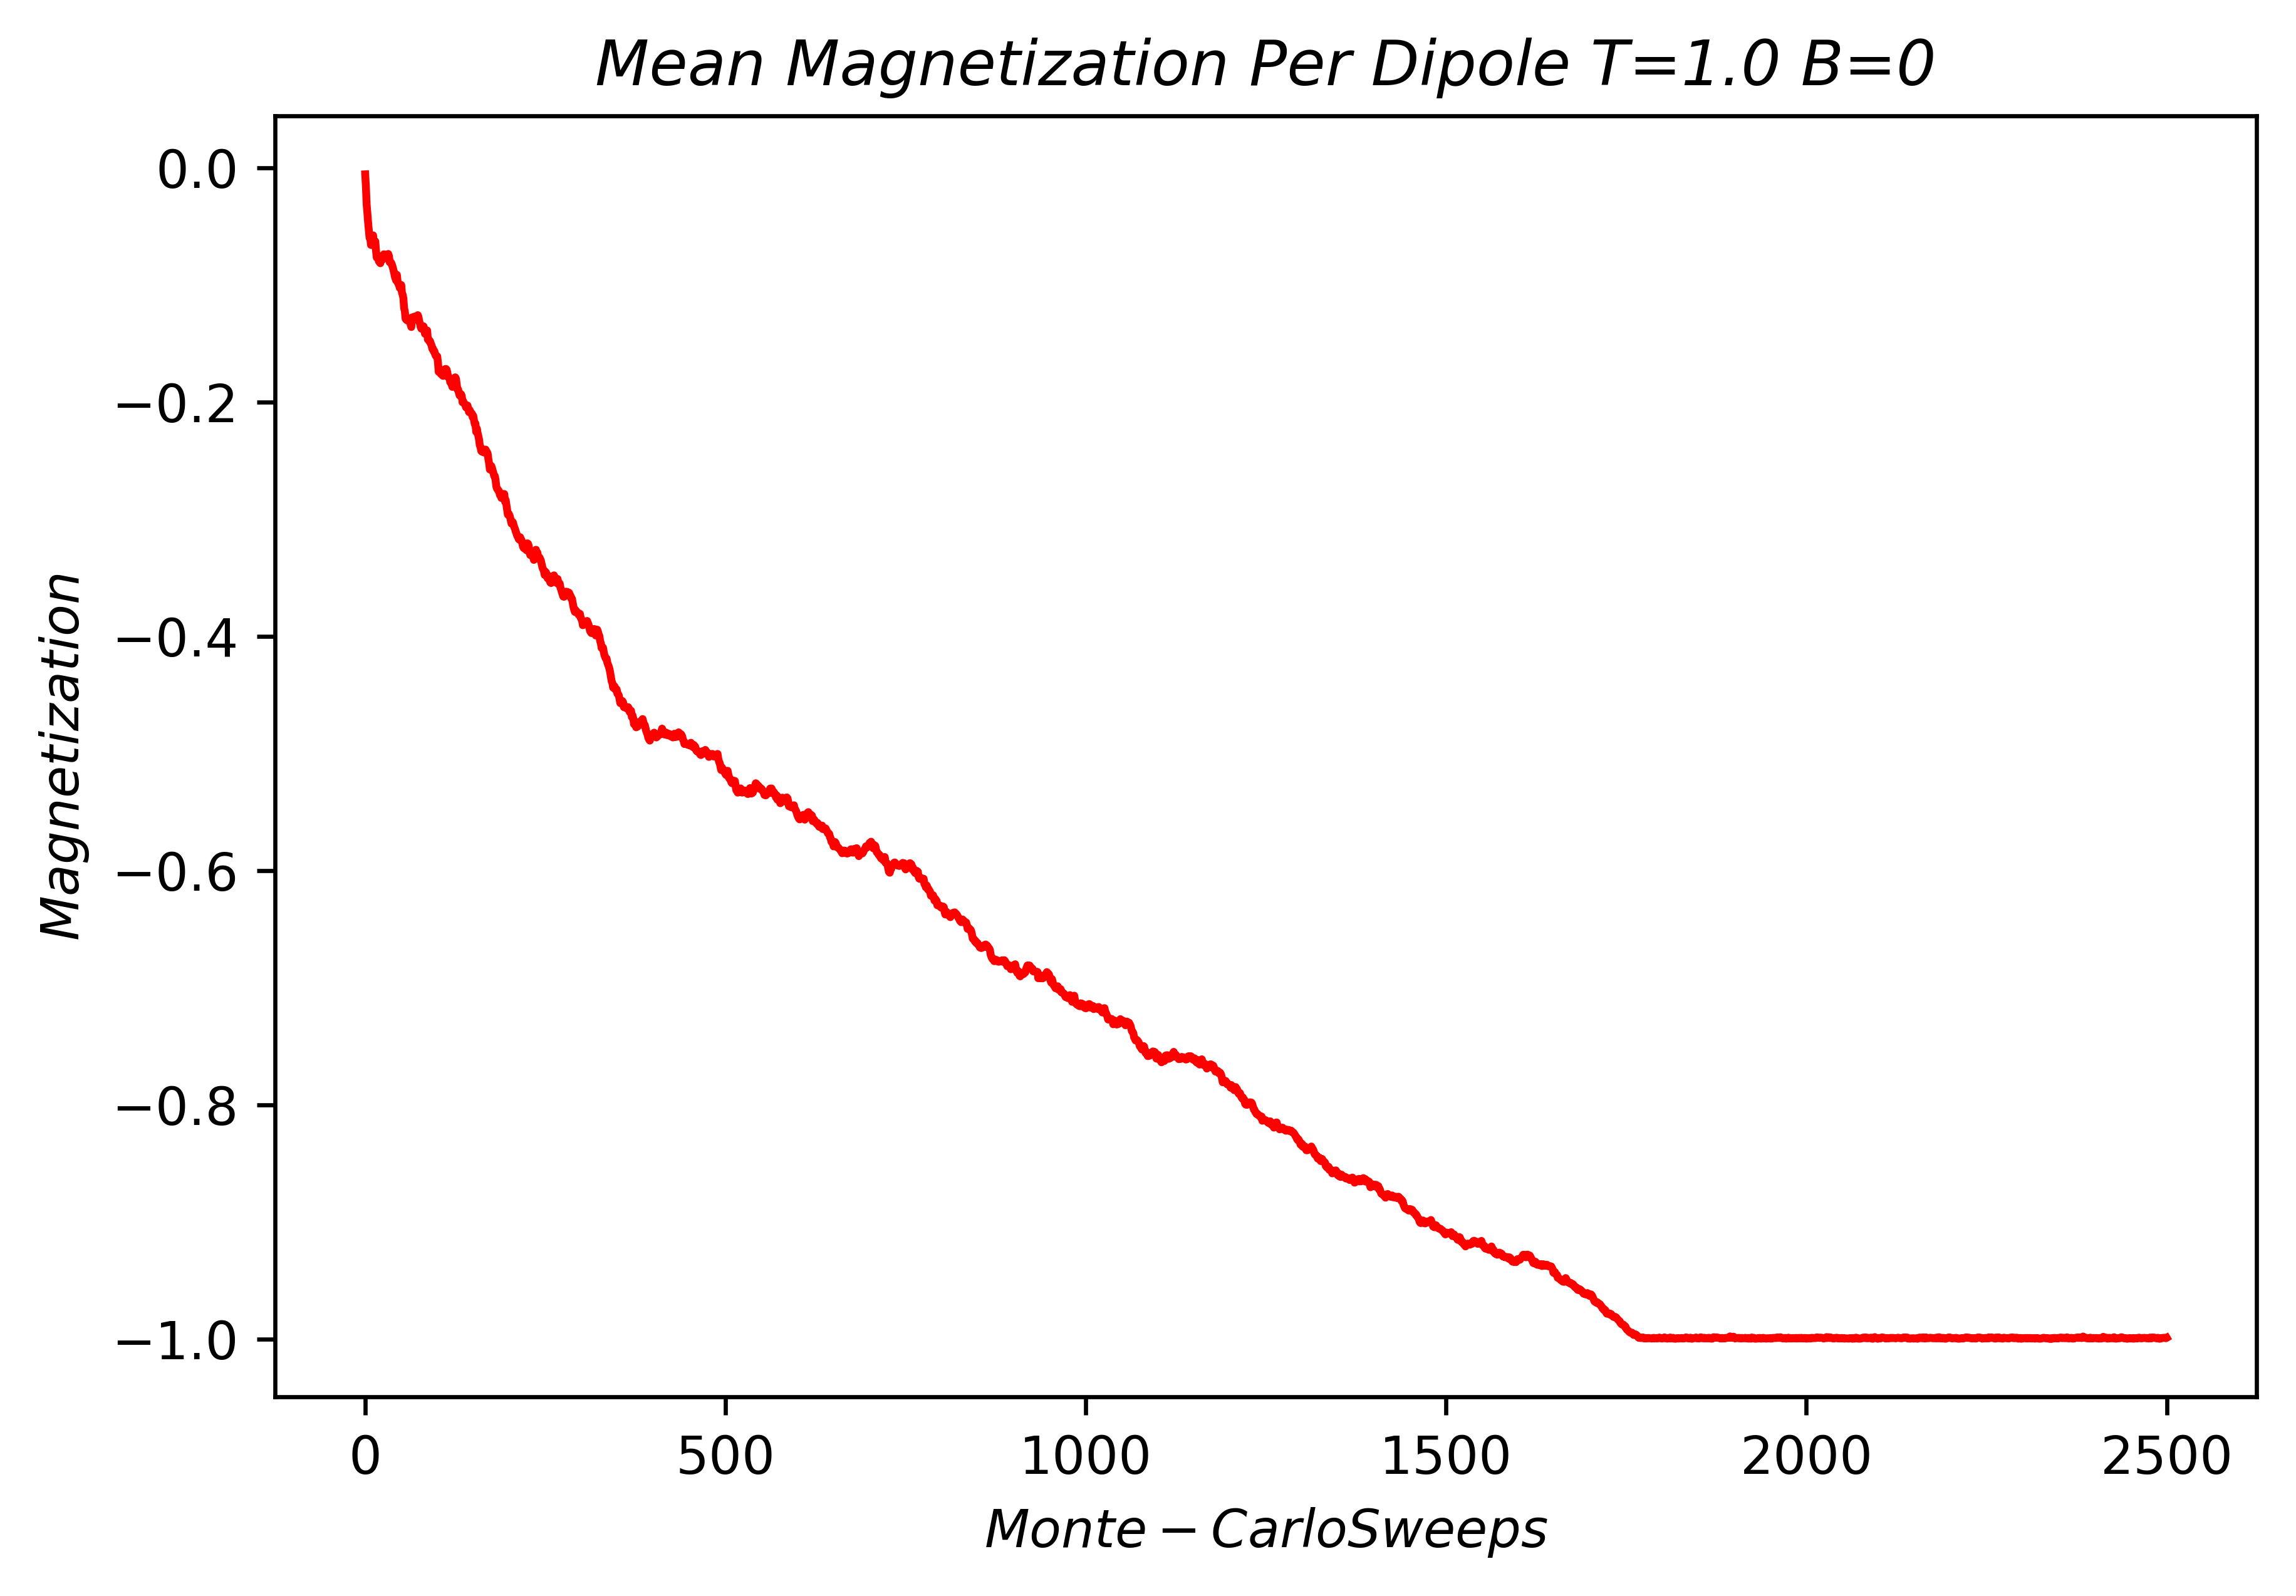
\includegraphics[scale=.5]{MagnetizationT=1B=0}
\end{figure}
\section{Experiment Two Analysis}
\hspace{\parindent}Part one of the second experiment sought to determine approximately how many Monte-Carlo sweeps were required to thermalize a randomly aligned Ising lattice at different temperatures, specifically for the cases: $T \ll T_c$, $T=T_c$, and $T \gg T_c$. In order to find this approximate value, the mean magnetization per dipole and the mean energy per dipole were observed as a function of time in Monte-Carlo sweeps to see if they ever appeared to come to an equilibrium of some sorts. In the case that $T \ll T_c$, complete thermalization occurred after 1750 Monte-Carlo sweeps, which is apparent in both the plot of the mean magnetization per dipole and the mean energy per dipole as seen in Figures (8) and (9). It should be noted though, that only after the first 500 Monte-Carlo sweeps that there was a distinct trend towards the equilibrium of the system found at 1750 Monte-Carlo sweeps. \\
%%%%%%%%%%%%%%%%%%%%%%%%%%%%%%%%%%%%%%%%%%%%%%%%%%%%%%%%%%%%
\begin{figure}[H]
\caption{This plot shows the evolution of $\overline{E}$ for a randomly aligned lattice in the case that $T=1 \ll T_c$. The evolution appears to be split into three distinct periods: prior to 500, $\overline{E}$ trends deeply downwards; after 500, it comes to a more consistent decrease; and post 1750, it plateaus indicating that thermalization has occured.}
\centering
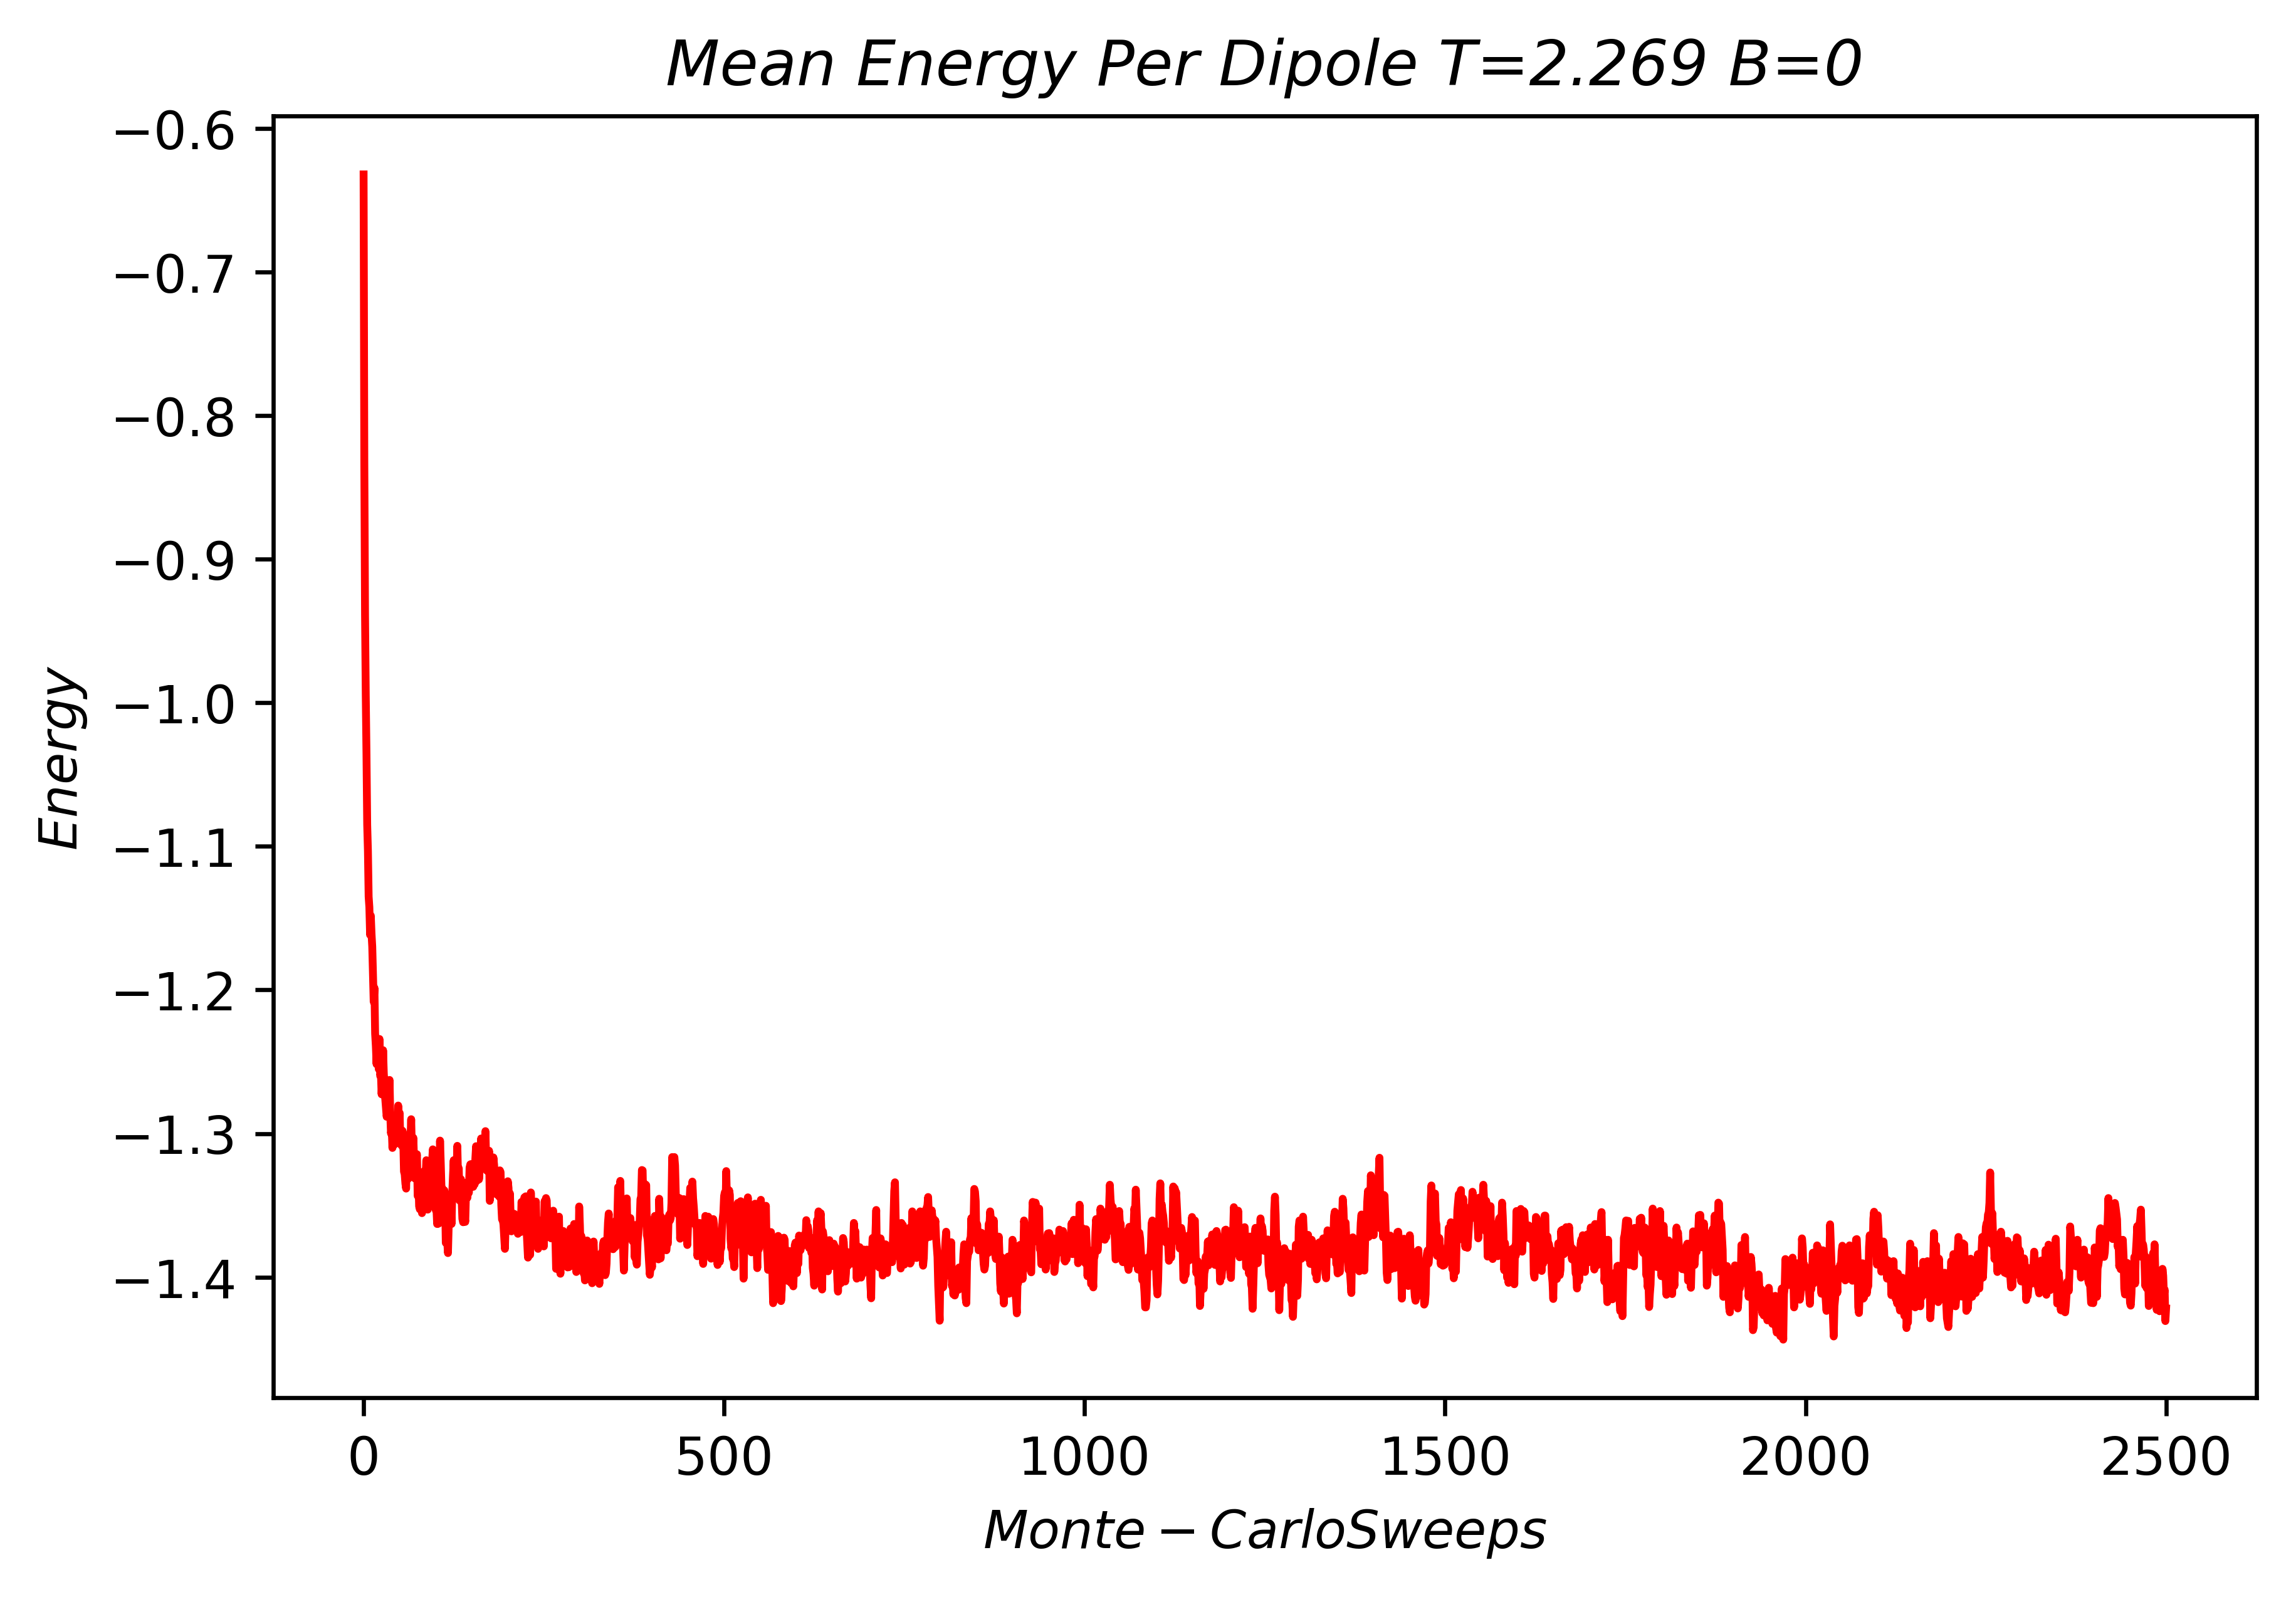
\includegraphics[scale=.5]{EnergyT=2269B=0}
\end{figure}
%%%%%%%%%%%%%%%%%%%%%%%%%%%%%%%%%%%%%%%%%%%%%%%%%%%%%%%%%%%%
In the case that $T = T_c$, complete thermalization occurred much more quickly than in the prior case, requiring only about 500 Monte-Carlo sweeps. This is apparent in both of its plots as seen in Figures (10) and (11) where both the mean magnetization per dipole and mean energy per dipole start to fluctuate about an equilibrium point.
%%%%%%%%%%%%%%%%%%%%%%%%%%%%%%%%%%%%%%%%%%%%%%%%%%%%%%%%%
\begin{figure}[H]
\caption{This plot shows the evolution of $\overline{m}$ for a randomly aligned lattice in the case that $T=2.269=T_c$. There seems to be no clear evolution even after 2500 sweeps which suggests that $\overline{m}$ simply tends to fluctuate around 0.}
\centering
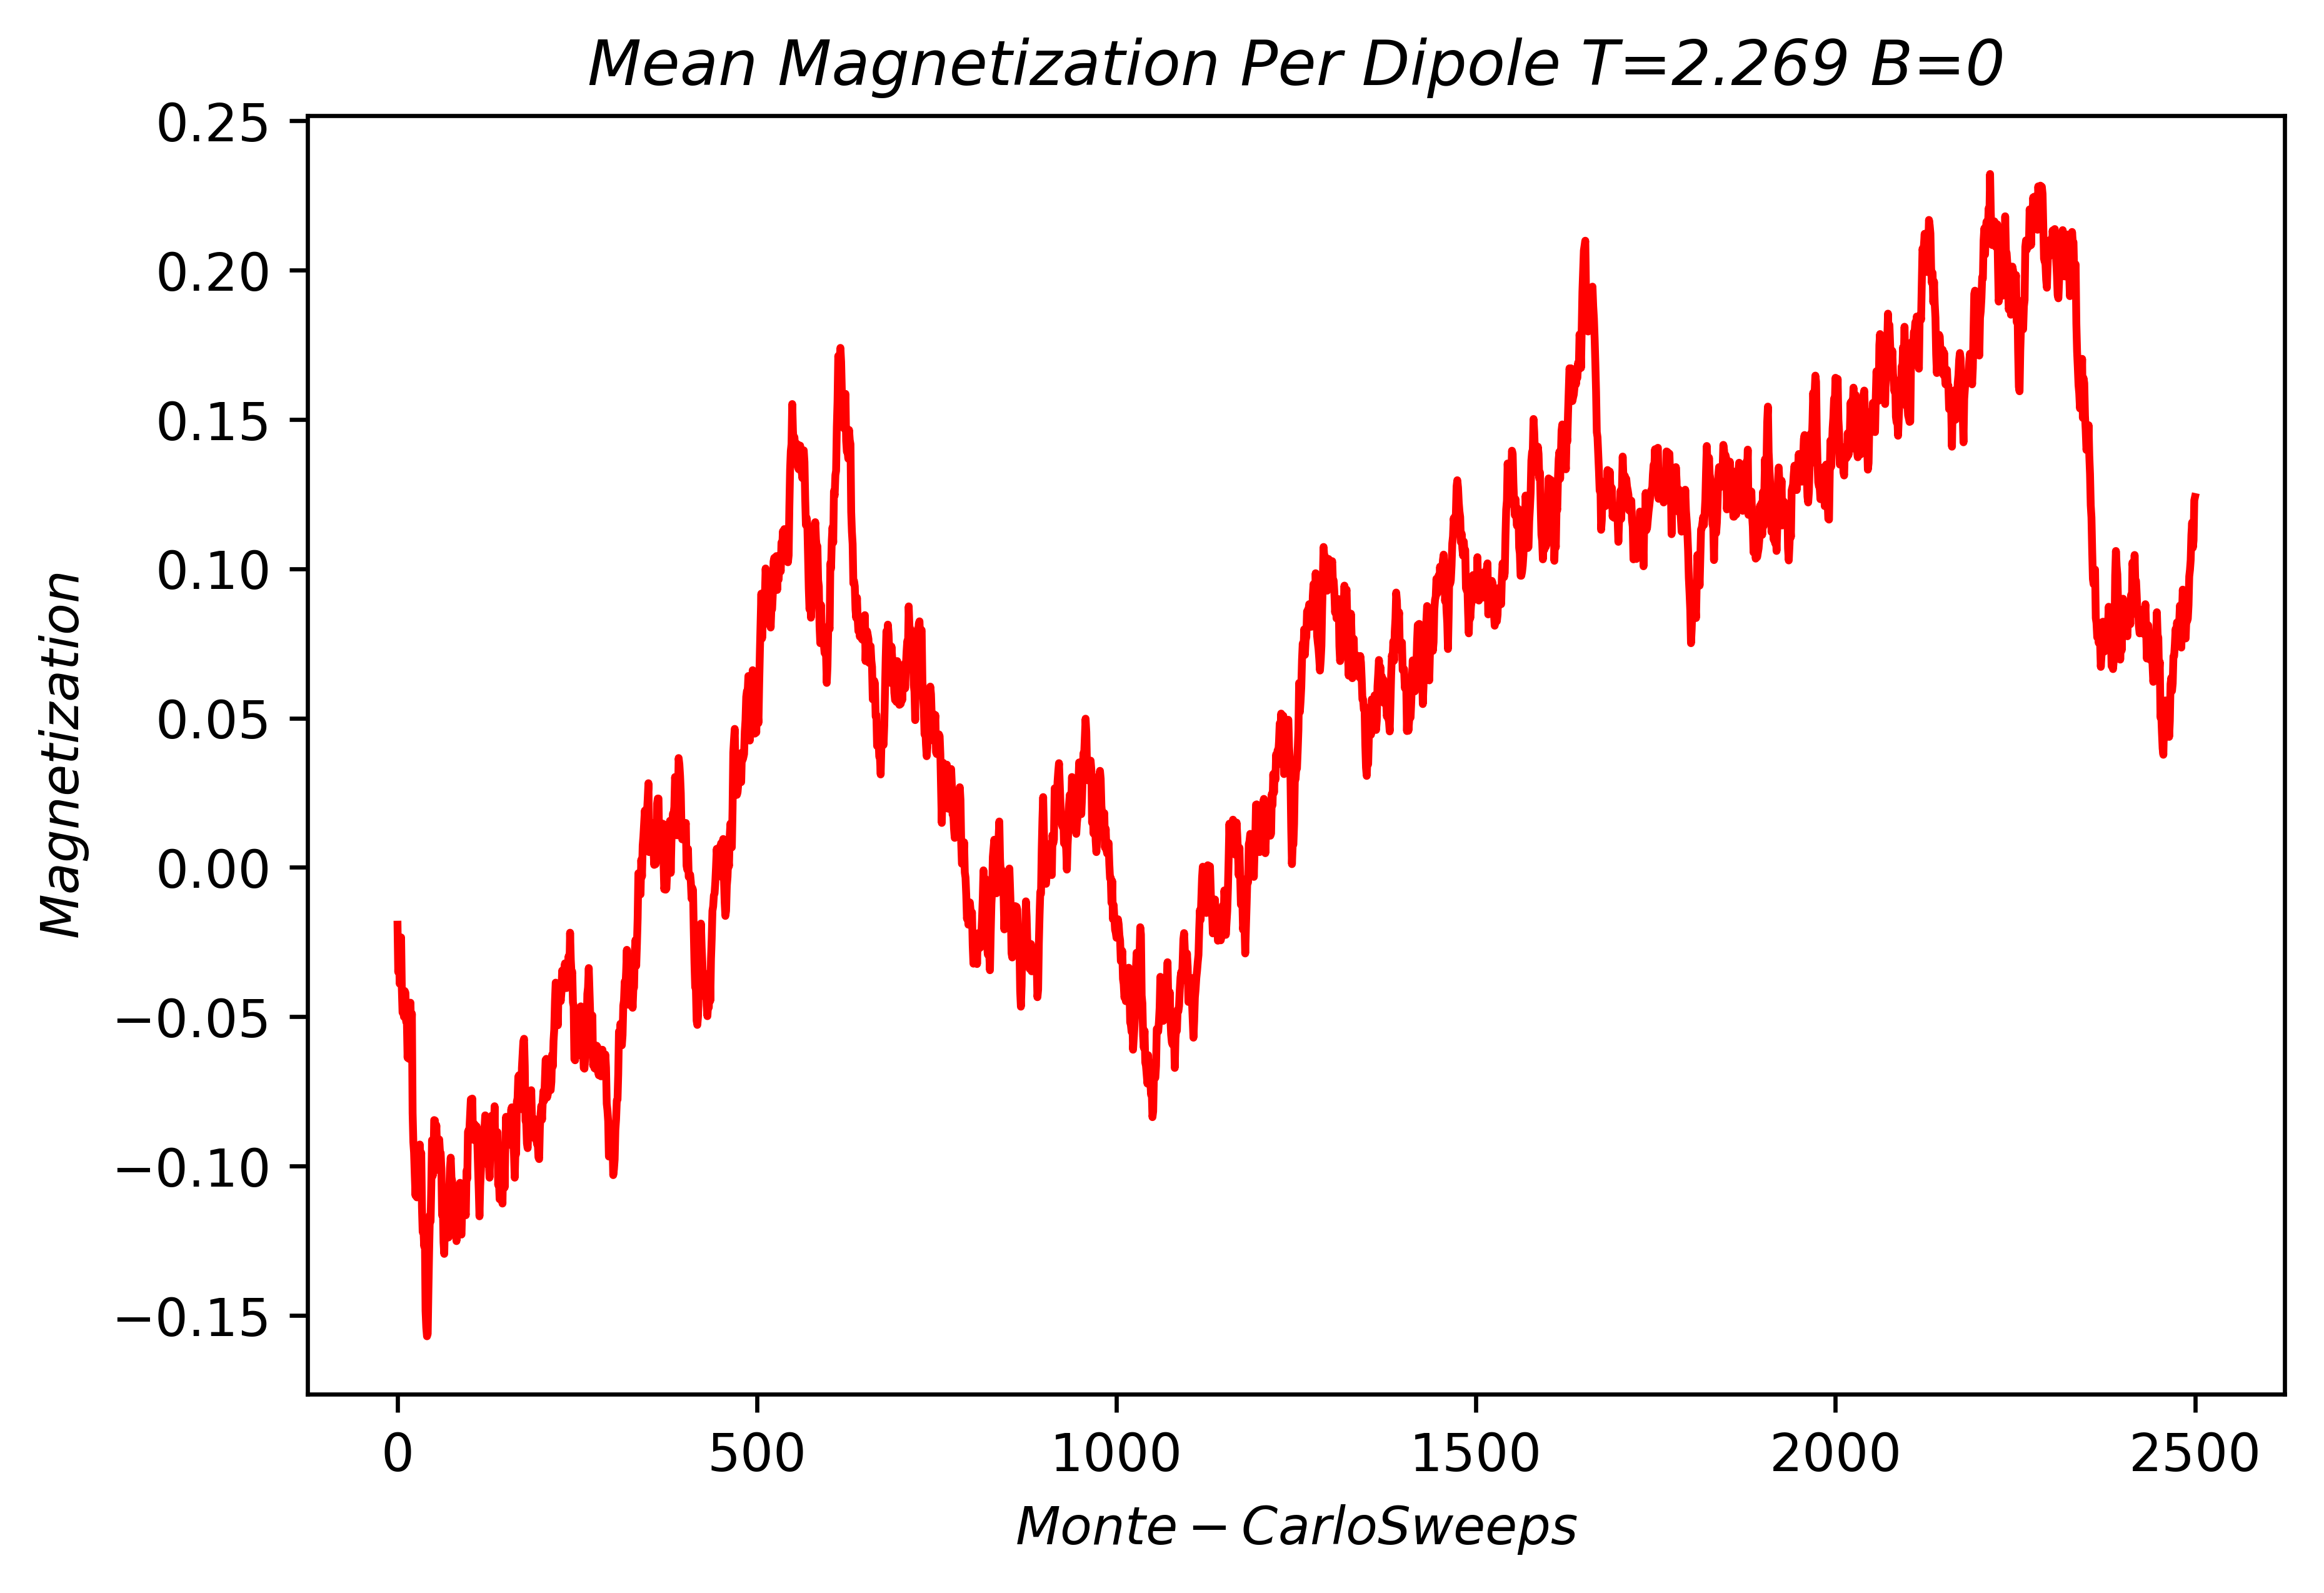
\includegraphics[scale=.5]{MagnetizationT=2269B=0}
%\end{figure}
%\begin{figure}[H]
\caption{This plot shows the evolution of $\overline{E}$ for a randomly aligned lattice in the case that $T=2.269=T_c$. The evolution appears to be split into two distinct periods: prior to 500, $\overline{E}$ trends deeply downwards, and afterwards fluctuates about an equilibrium point indicating that thermalization has occurred.}
\centering
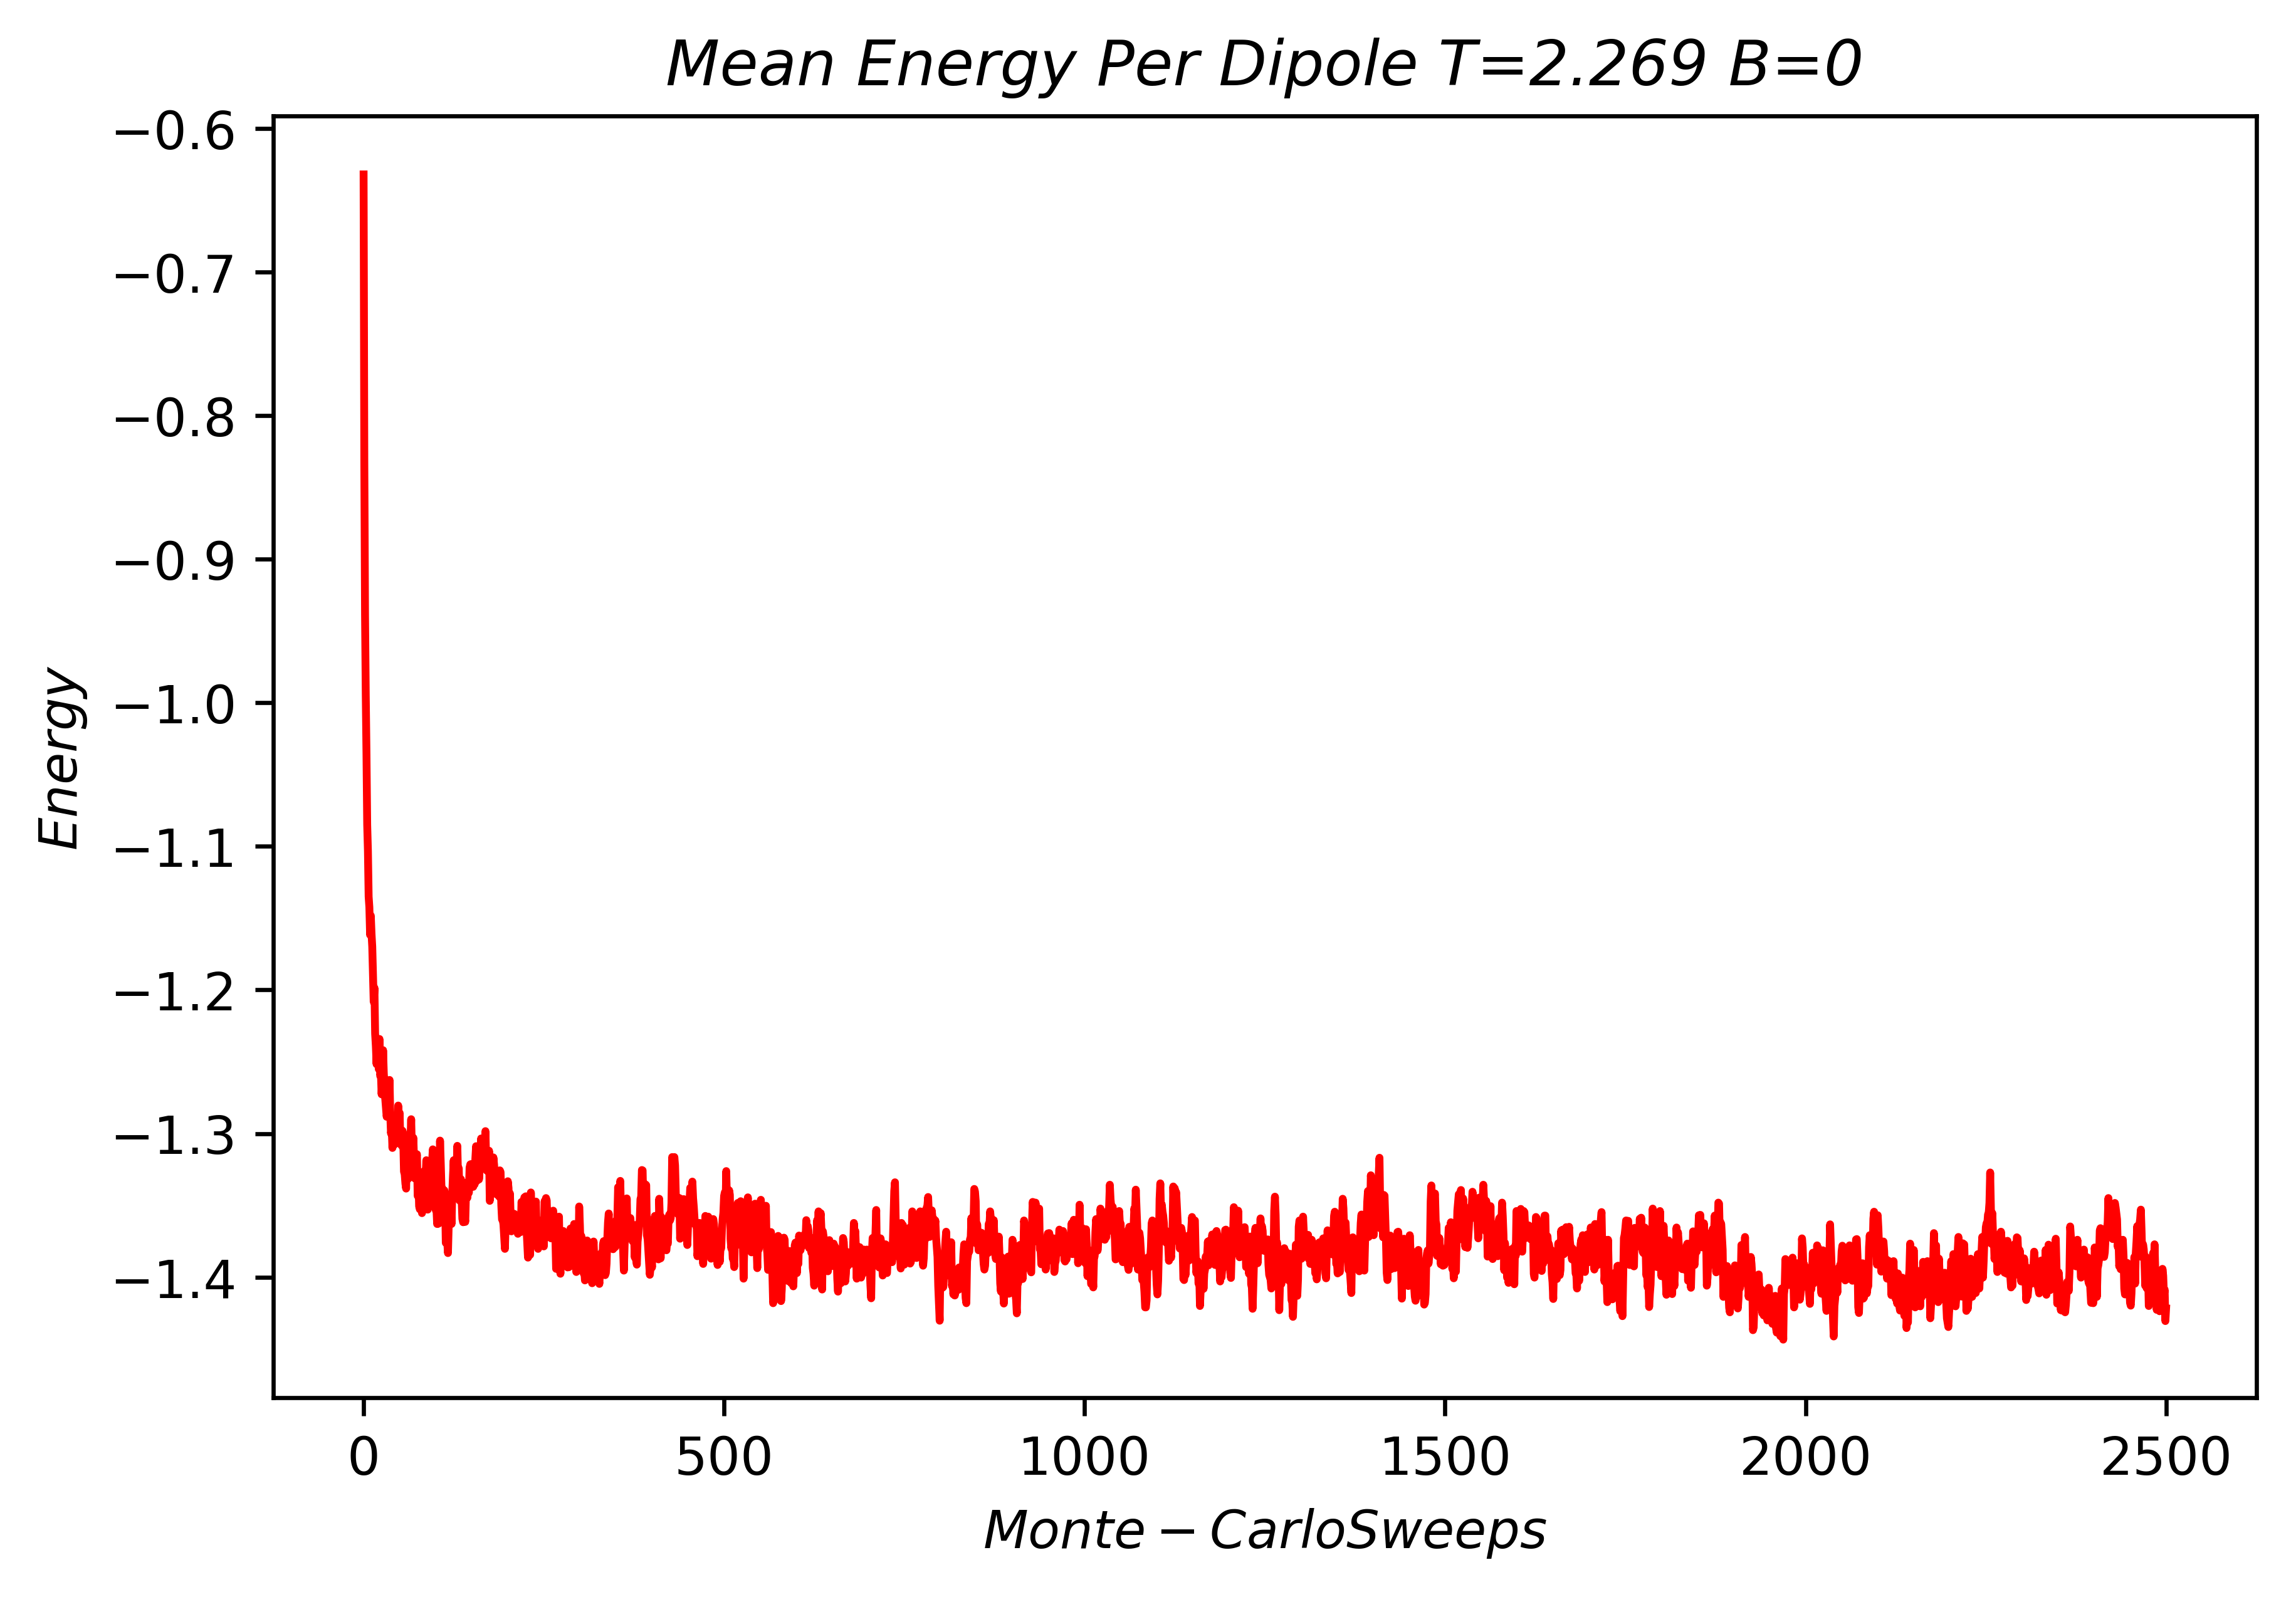
\includegraphics[scale=.5]{EnergyT=2269B=0}
\end{figure}
%%%%%%%%%%%%%%%%%%%%%%%%%%%%%%%%%%%%%%%%%%%%%%%%%%%%%%%%%%%%
In the final case, where $T \gg T_c$, complete thermalization was nearly instantaneous. After only a few sweeps both the mean magnetization per dipole and the mean energy per dipole began fluctuating about what are clearly there equilibrium points. In Figure (12) the mean magnetization fluctuates about zero, which is predictable considering the lattice should no longer be ferromagnetic at this temperature hence should have no preferred alignment unlike the previous two cases. Figure (13) also shows this same behavior in the energy domain. \\
%%%%%%%%%%%%%%%%%%%%%%%%%%%%%%%%%%%%%%%%%%%%%%%%%%%%%%%%%%%%
\begin{figure}[H]
\caption{This plot shows the evolution of $\overline{m}$ for a randomly aligned lattice in the case that $T\gg T_c$. There is very little evolution in the lattice over time and simply fluctuates about zero indicating that thermalization is extremely rapid.}
\centering
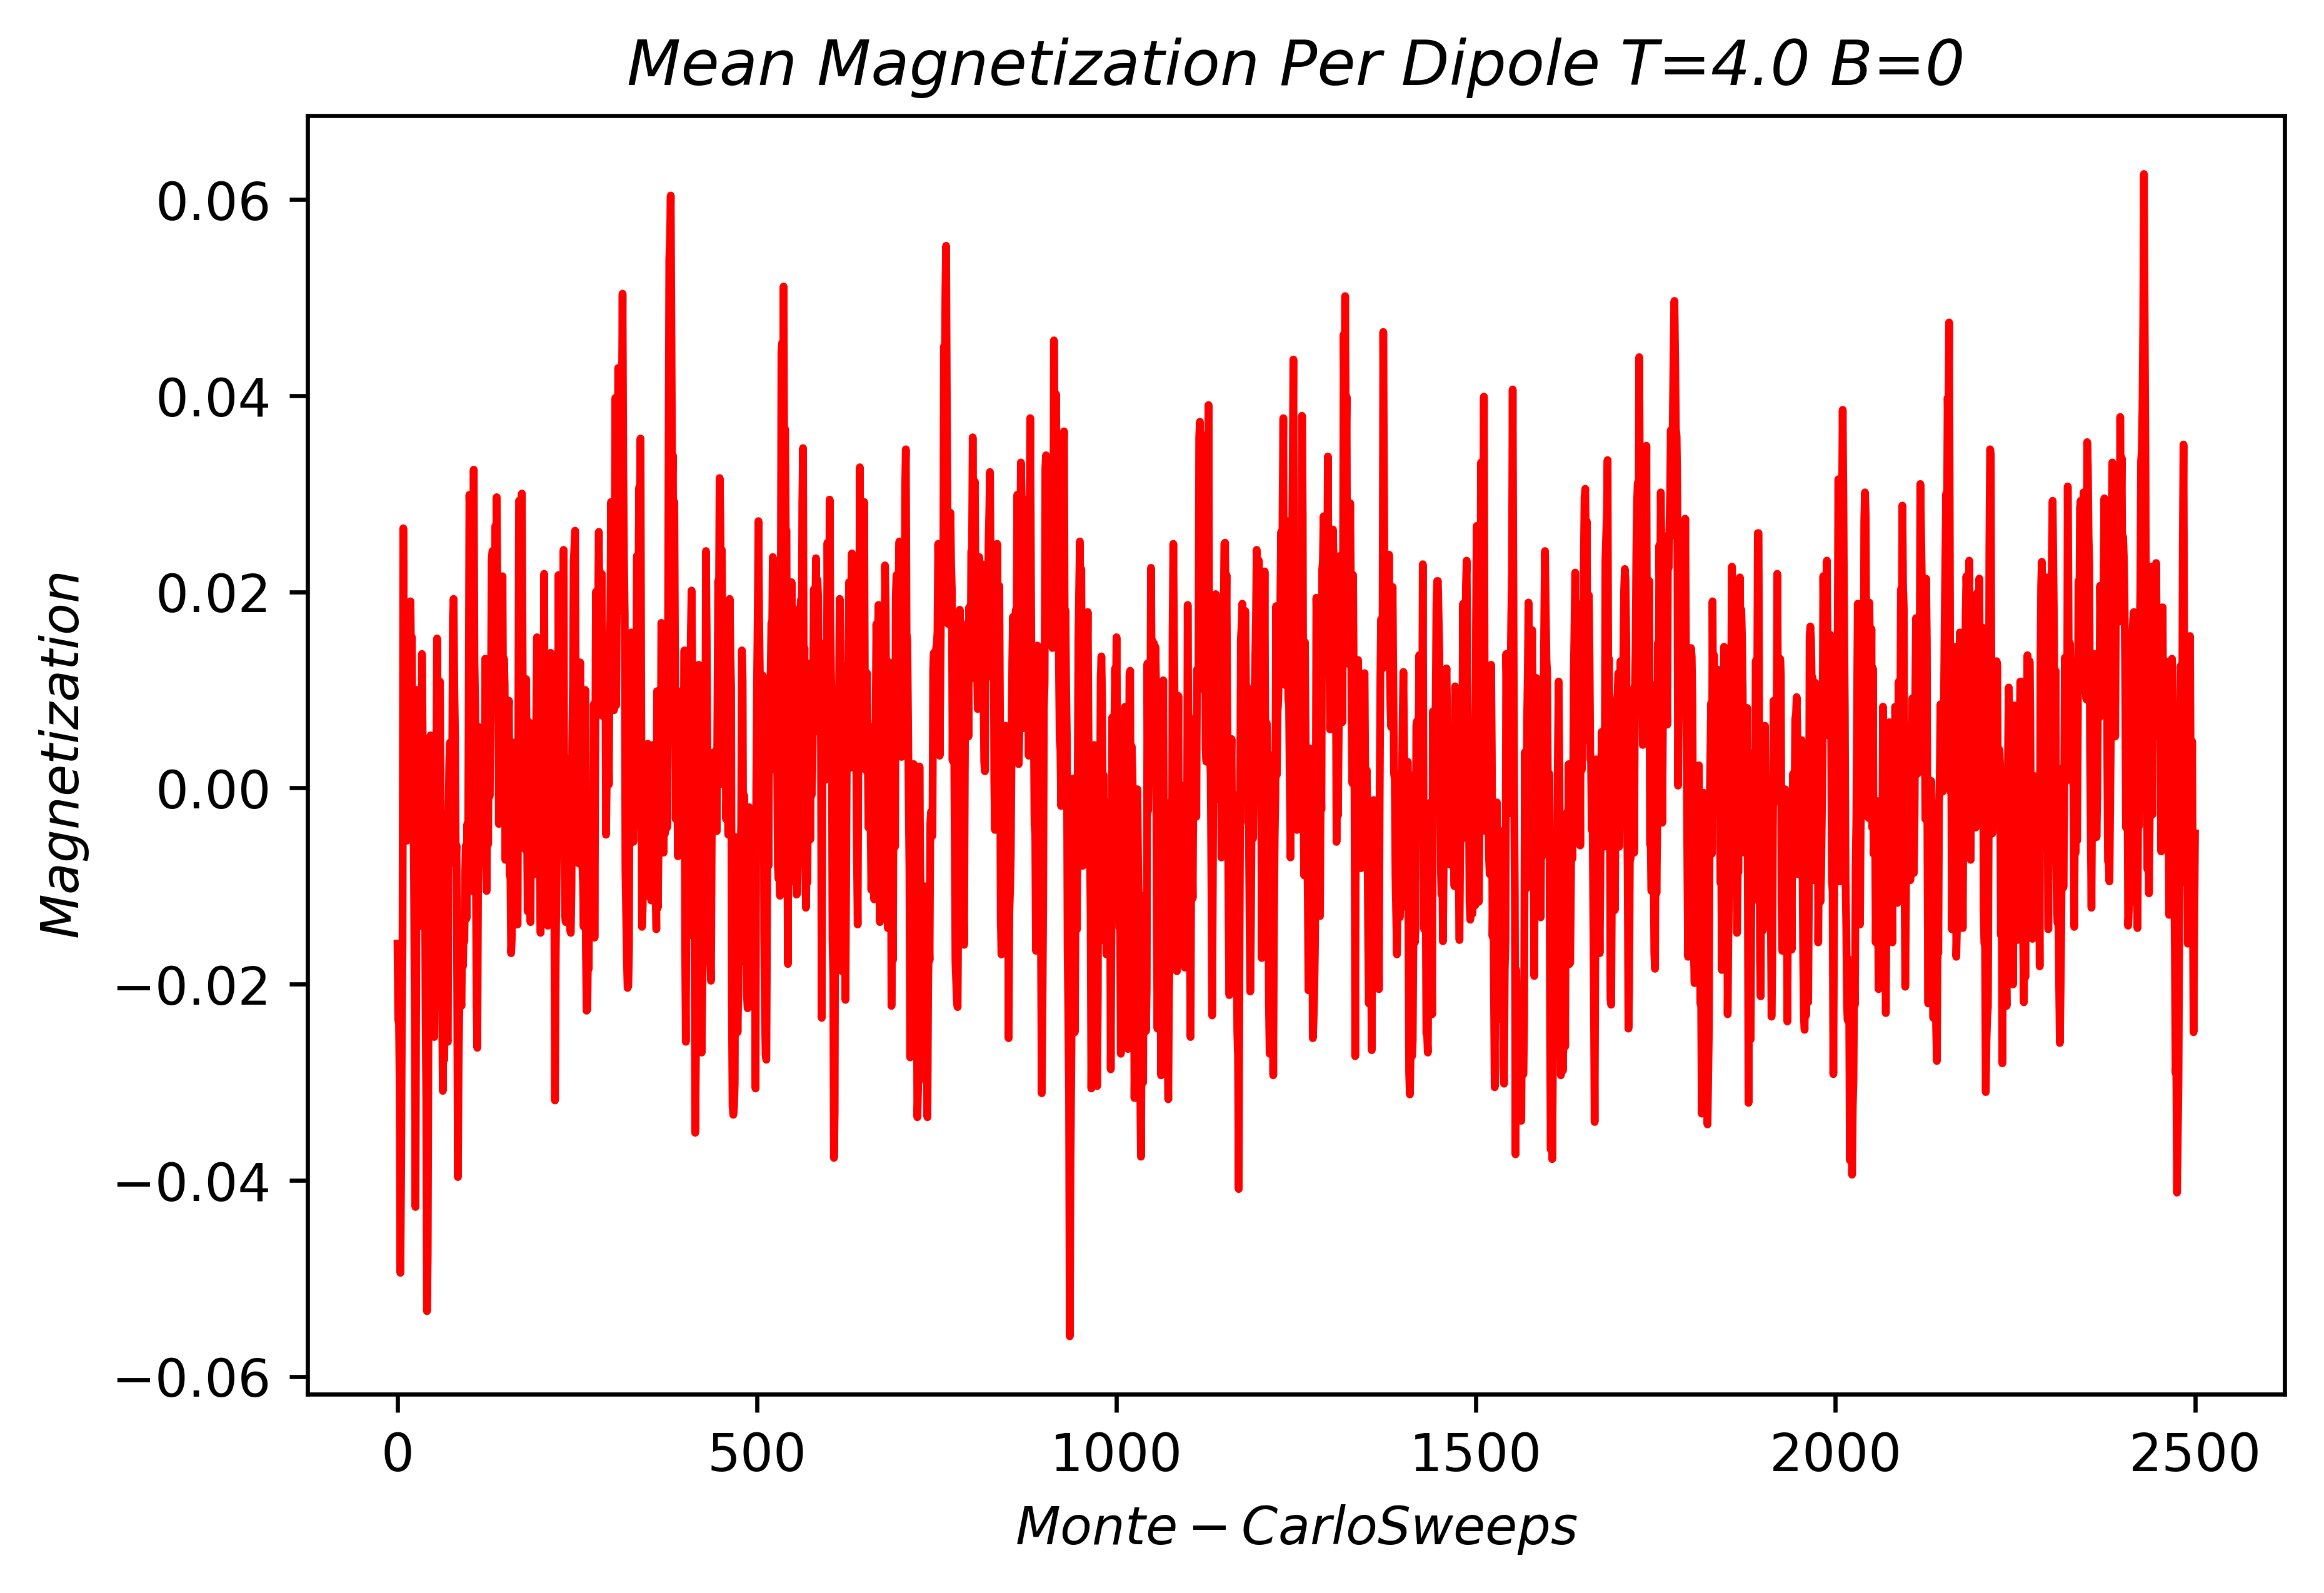
\includegraphics[scale=.5]{MagnetizationT=4B=0}
\end{figure}
\begin{figure}[ht]
\caption{This plot shows the evolution of $\overline{E}$ for a randomly aligned lattice in the case that $T\gg =T_c$. The evolution is very rapid at first, but quickly comes to fluctuate about an equilibrium point. This indicates that the thermalization at temperatures above $T_c$ occurs very rapidly.}
\centering
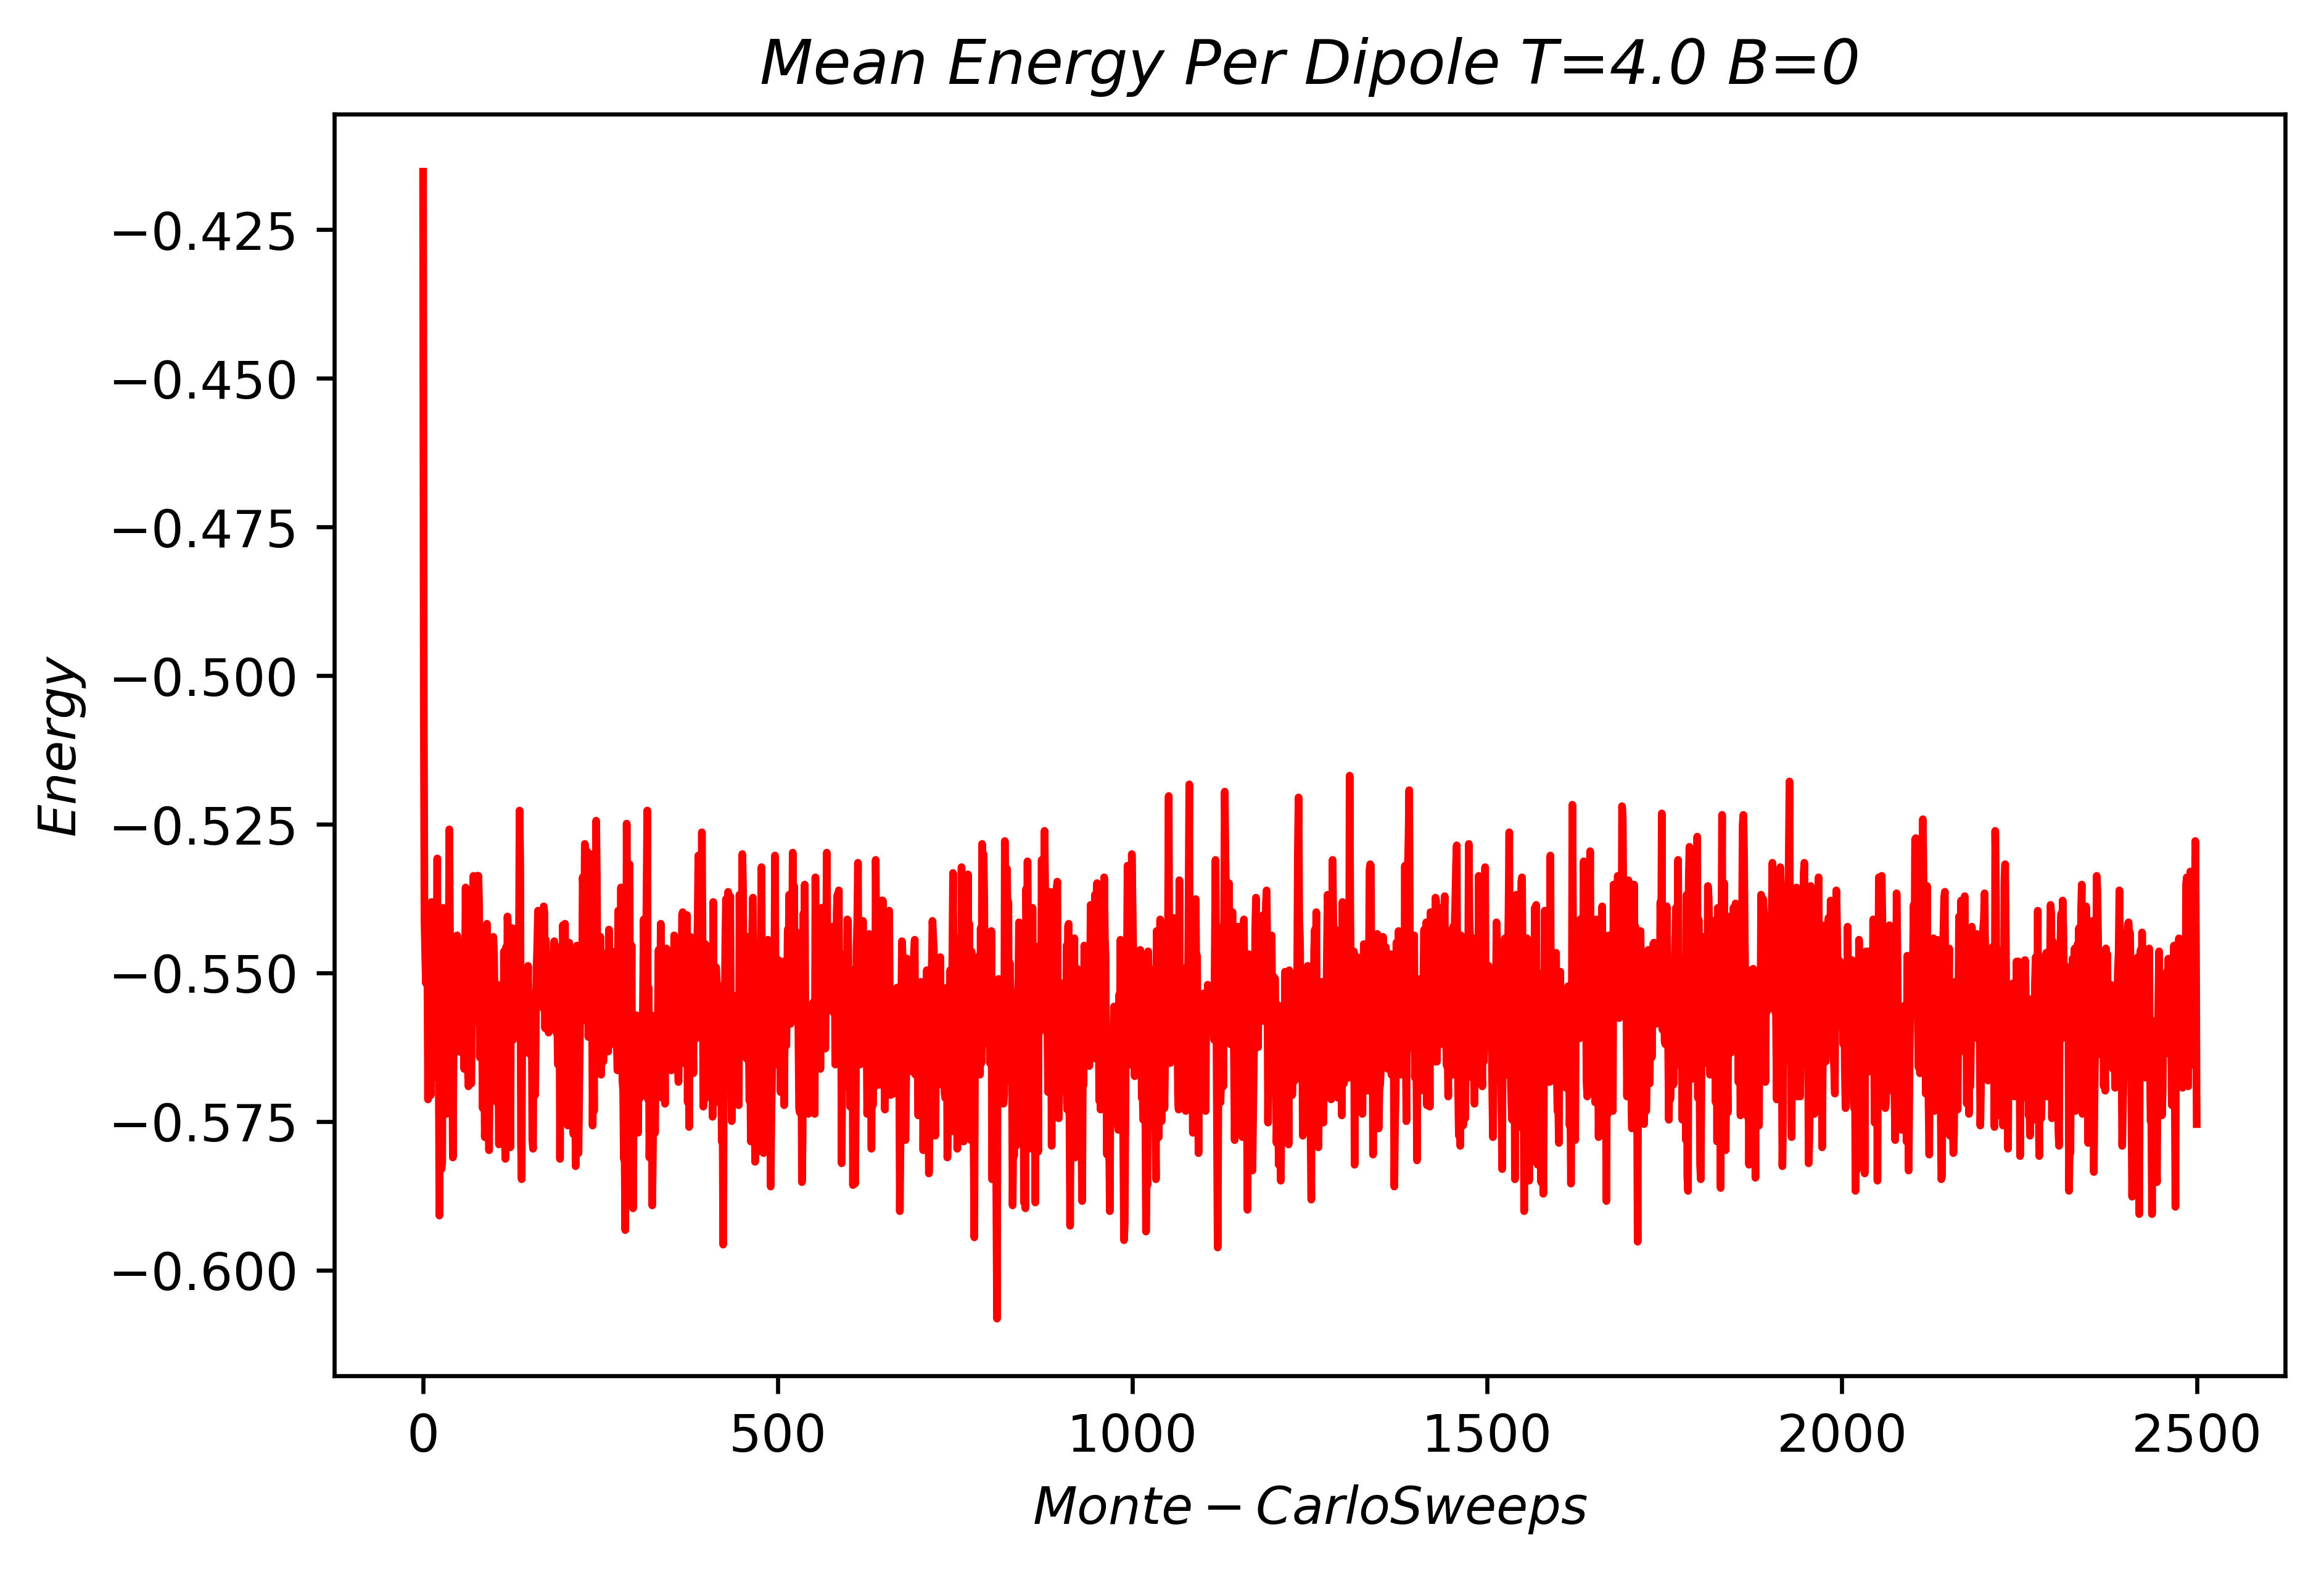
\includegraphics[scale=.5]{EnergyT=4B=0}
\end{figure}
%%%%%%%%%%%%%%%%%%%%%%%%%%%%%%%%%%%%%%%%%%%%%%%%%%%%%%%%%%%%
On a final note in regards to this portion of experiment two, it is valuable to observe how the lattice actually looks after the 2500 Monte-Carlo sweeps. This is an important observation because it gives direct insight towards how the dipoles interact with each other about the critical temperature. In the case that the temperature of the external heat bath is below the critical temperature the lattice is clearly dominated by one alignment of the dipoles as seen in Figure (14). In the case that the temperature of the external heat bath is greater than the critical temperature the lattice has no structure at all and is completely random as seen in Figure (15) - a property that should be expected considering that the lattice should no longer be a ferro-magnet. In the final case, where the temperature is equal to the critical temperature there exists small structures within the lattice. These structures are certainly not on the scale as seen in Figure(14), however they are definitely not random either as seen in Figure (15). Hence, Figure (16) appears to show exactly what would be predicted of the lattice at the critical temperature. \\
%%%%%%%%%%%%%%%%%%%%%%%%%%%%%%%%%%%%%%%%%%%%%%%%%%%%%%%%%%%%
\begin{figure}[H]
\caption{$T=1\ll =T_c$}
\centering
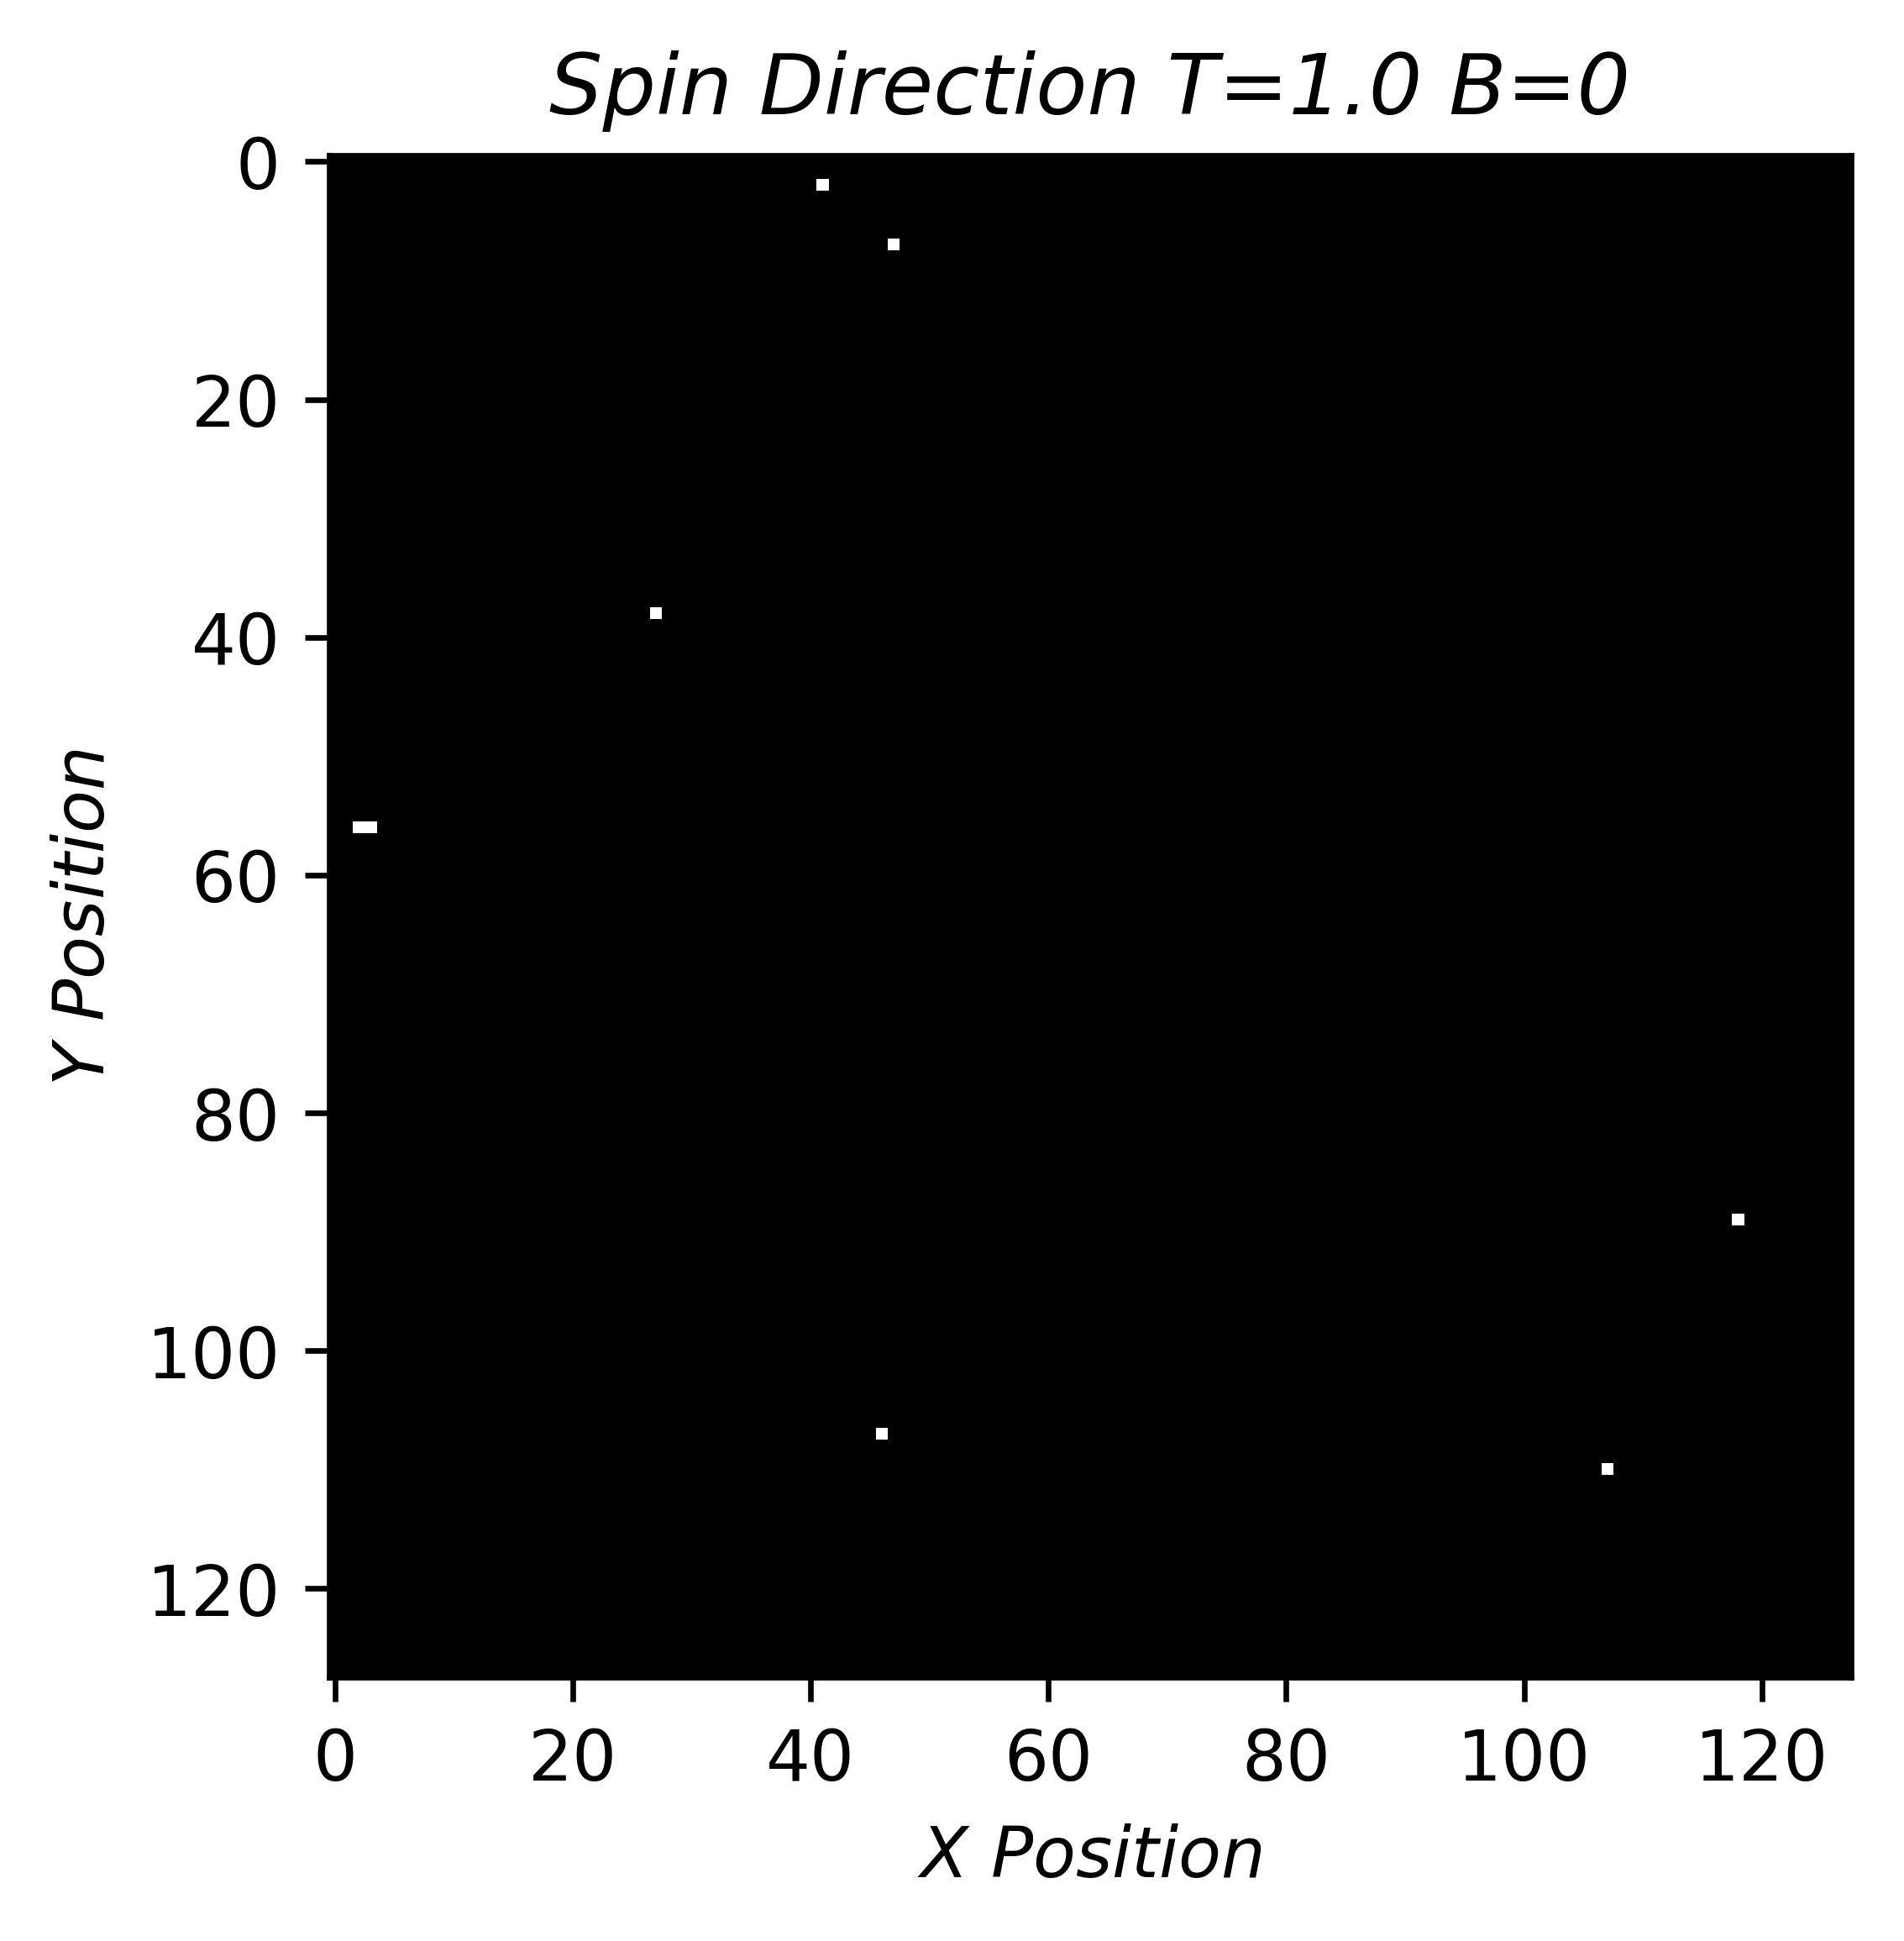
\includegraphics[scale=.6]{SpinsT=1B=0}
%\end{figure}
%\begin{figure}[]
\caption{$T=2.269=T_c$ }
\centering
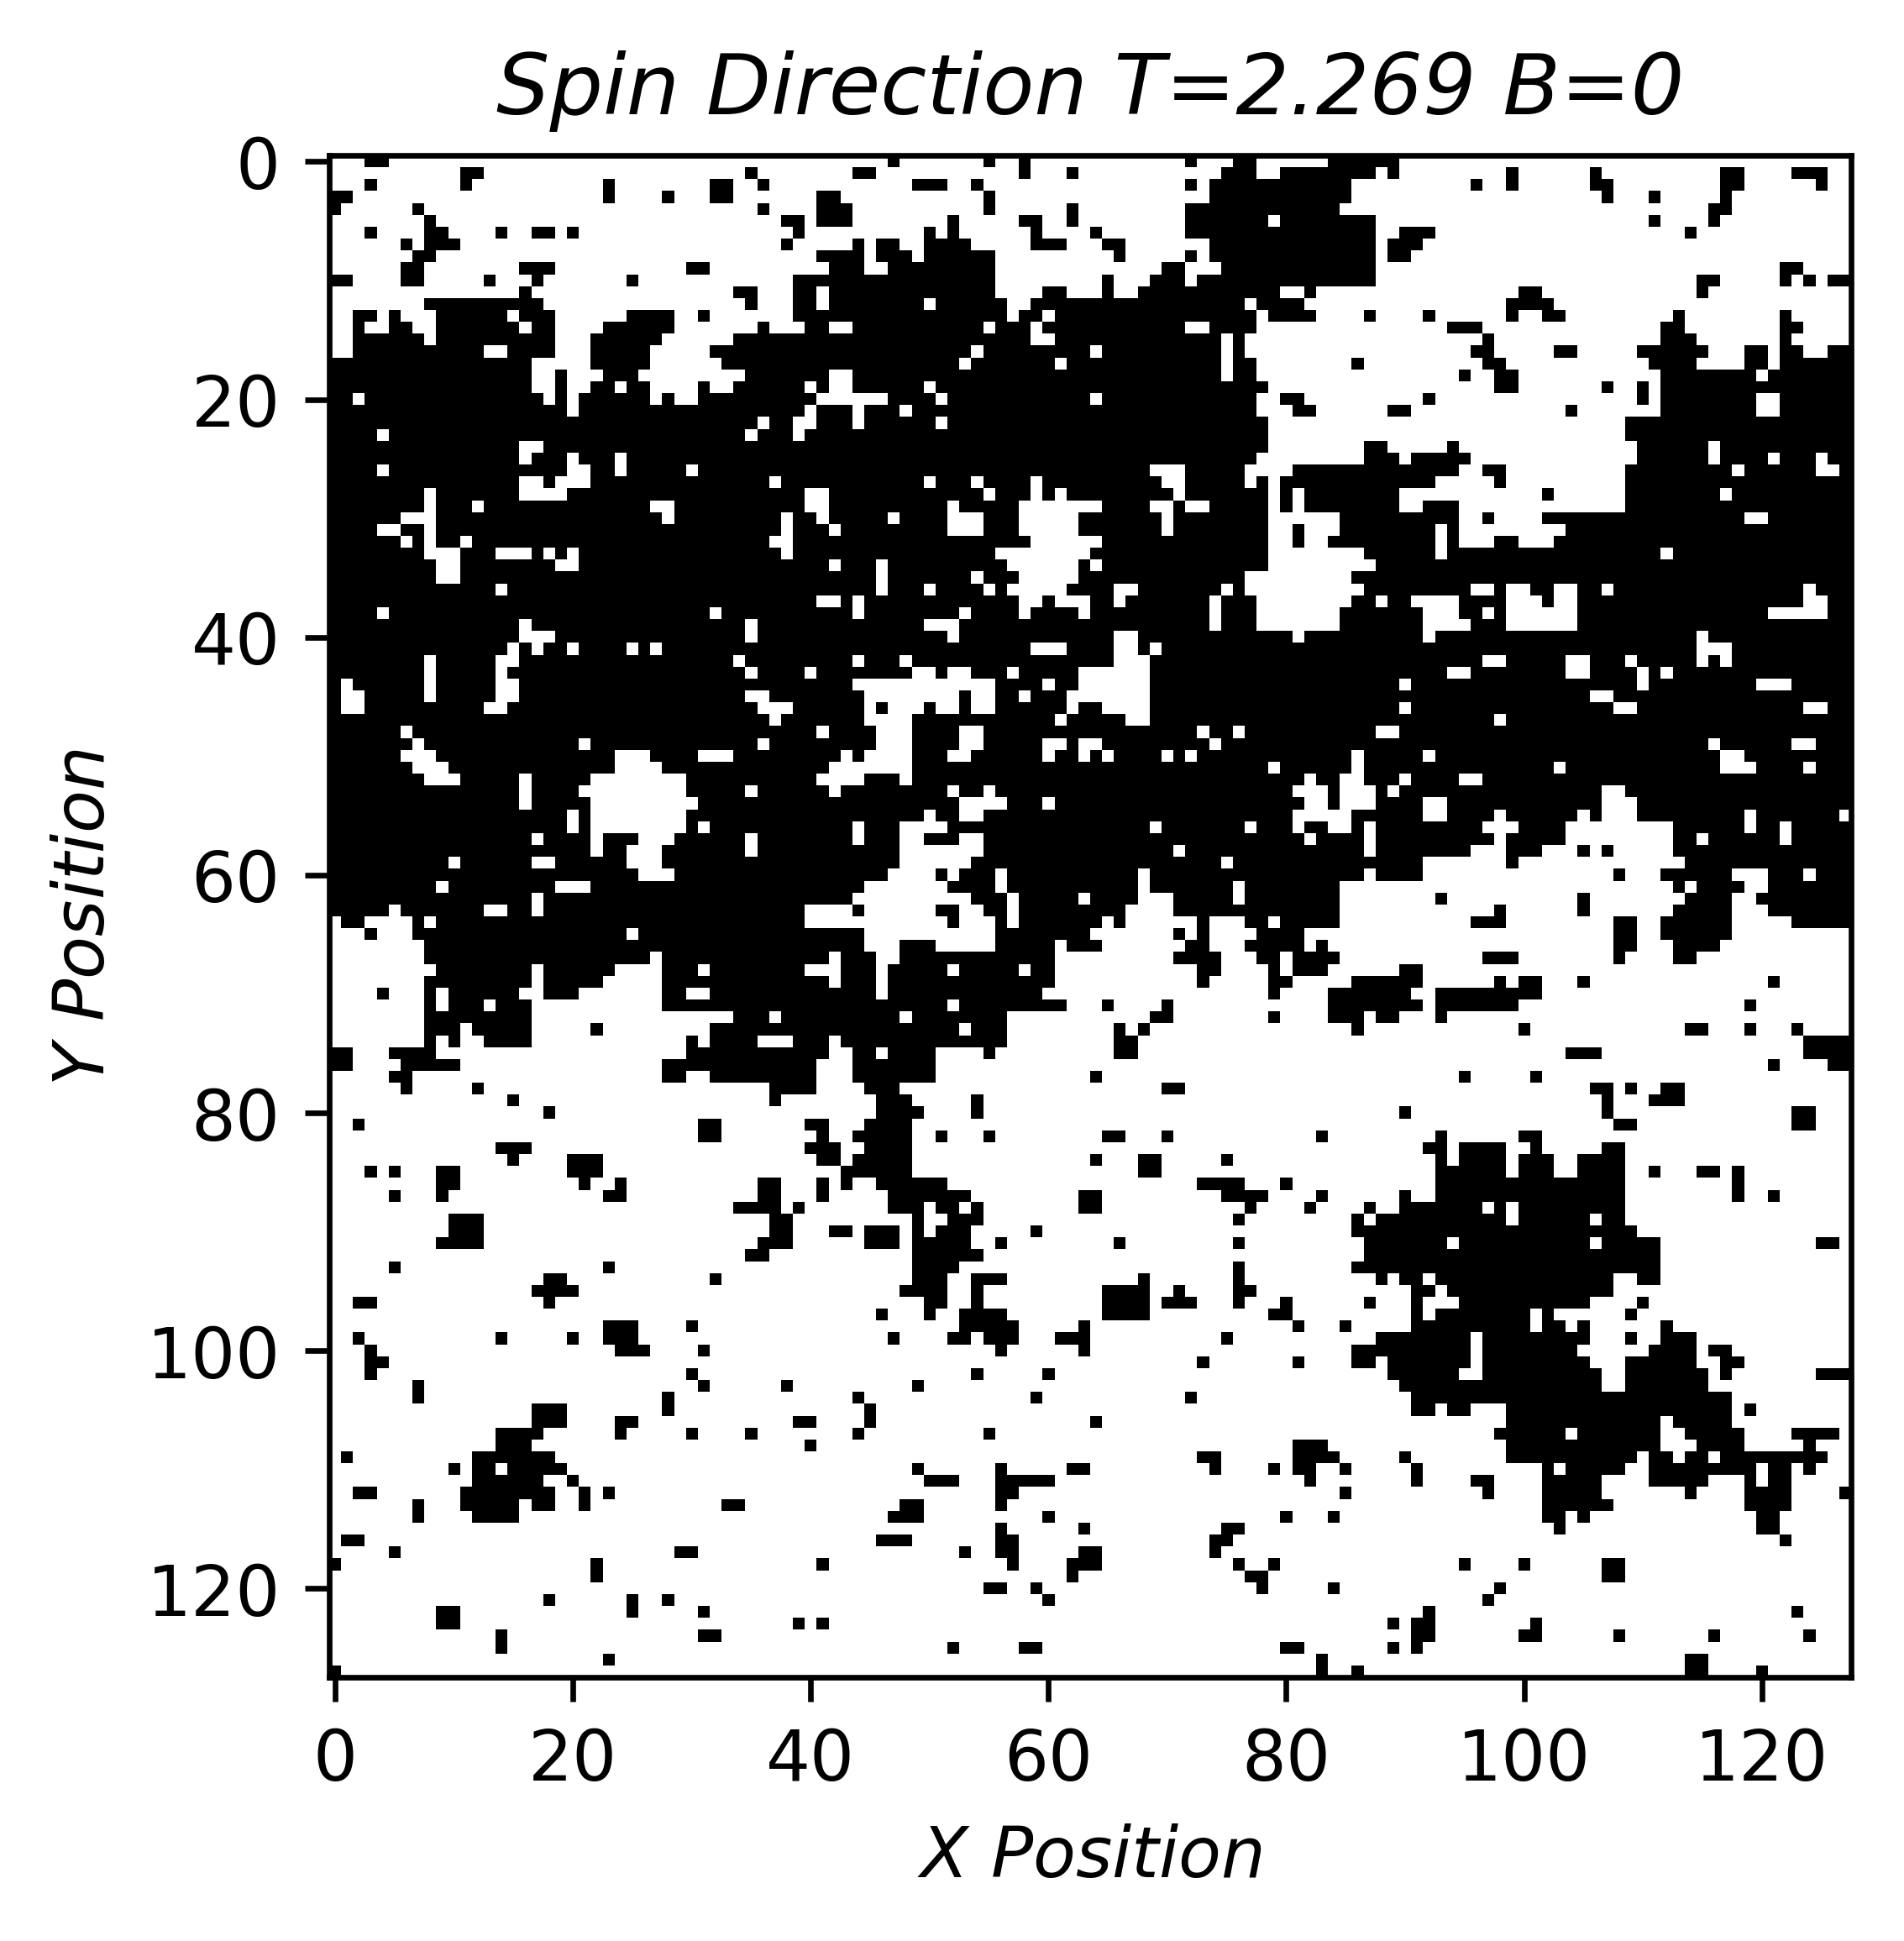
\includegraphics[scale=.6]{SpinsT=2269B=0}
%\end{figure}
%\begin{figure}[]
\caption{$T=4\gg =T_c$ }
\centering
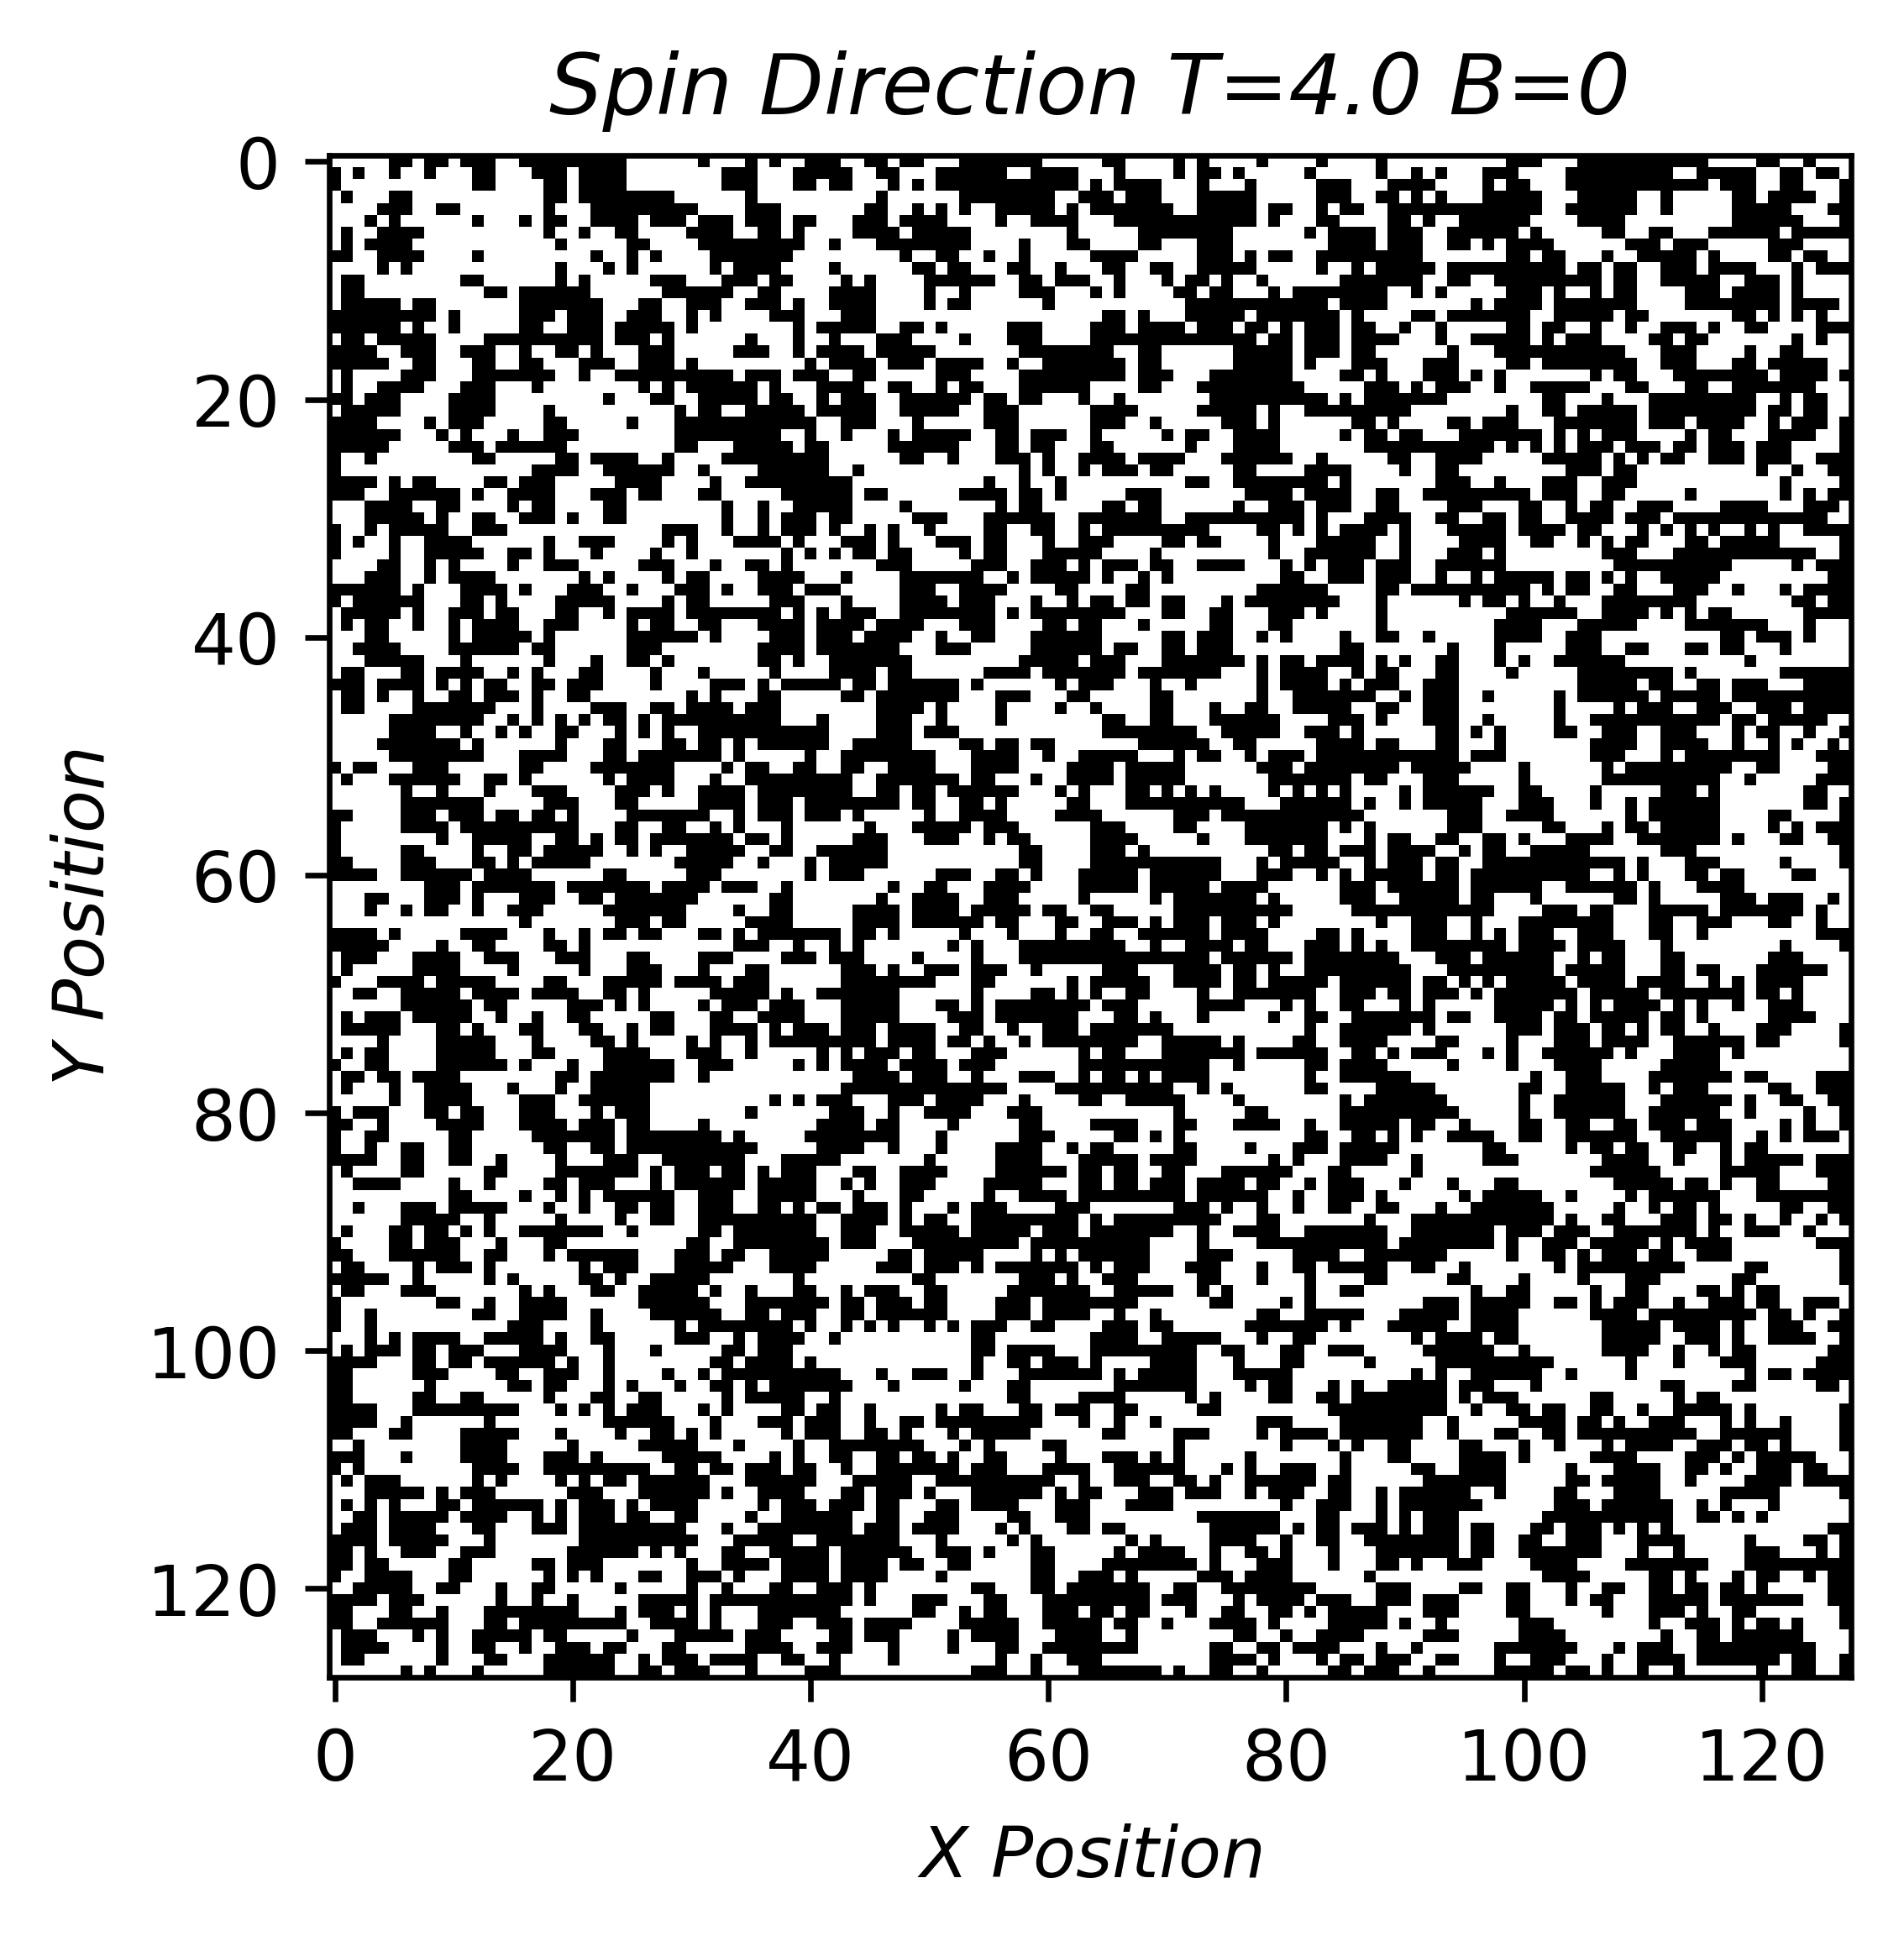
\includegraphics[scale=.6]{SpinsT=4B=0}
\end{figure}
%%%%%%%%%%%%%%%%%%%%%%%%%%%%%%%%%%%%%%%%%%%%%%%%%%%%%%%%%%%%
Part two of the second experiment sought to explore the relationship between specific heat capacity per spin and the magnetic susceptibility per spin as a function of different temperatures about the critical temperature and as a function of different lattice sizes. The objective was to search for a peak or divergence using both of these quantities to determine whether a second order phase transition occurs or not. The smallest lattice, which was [32 X 32], exhibits peaks for both the specific heat capacity per spin and the magnetic susceptibility per spin about $T_c$ as seen in Figures (17) and (18), which is good as it indicates that there is likely a second order phase transition occurring even with such a small lattice. The jaggedness of both plots though, is not expected and presumably should become smoother with larger lattices.\\
%%%%%%%%%%%%%%%%%%%%%%%%%%%%%%%%%%%%%%%%%%%%%%%%%%%%%%%%%%%%
\begin{figure}[H]
\caption{Magnetic Susceptibility for [32 X 32] lattice}
\centering
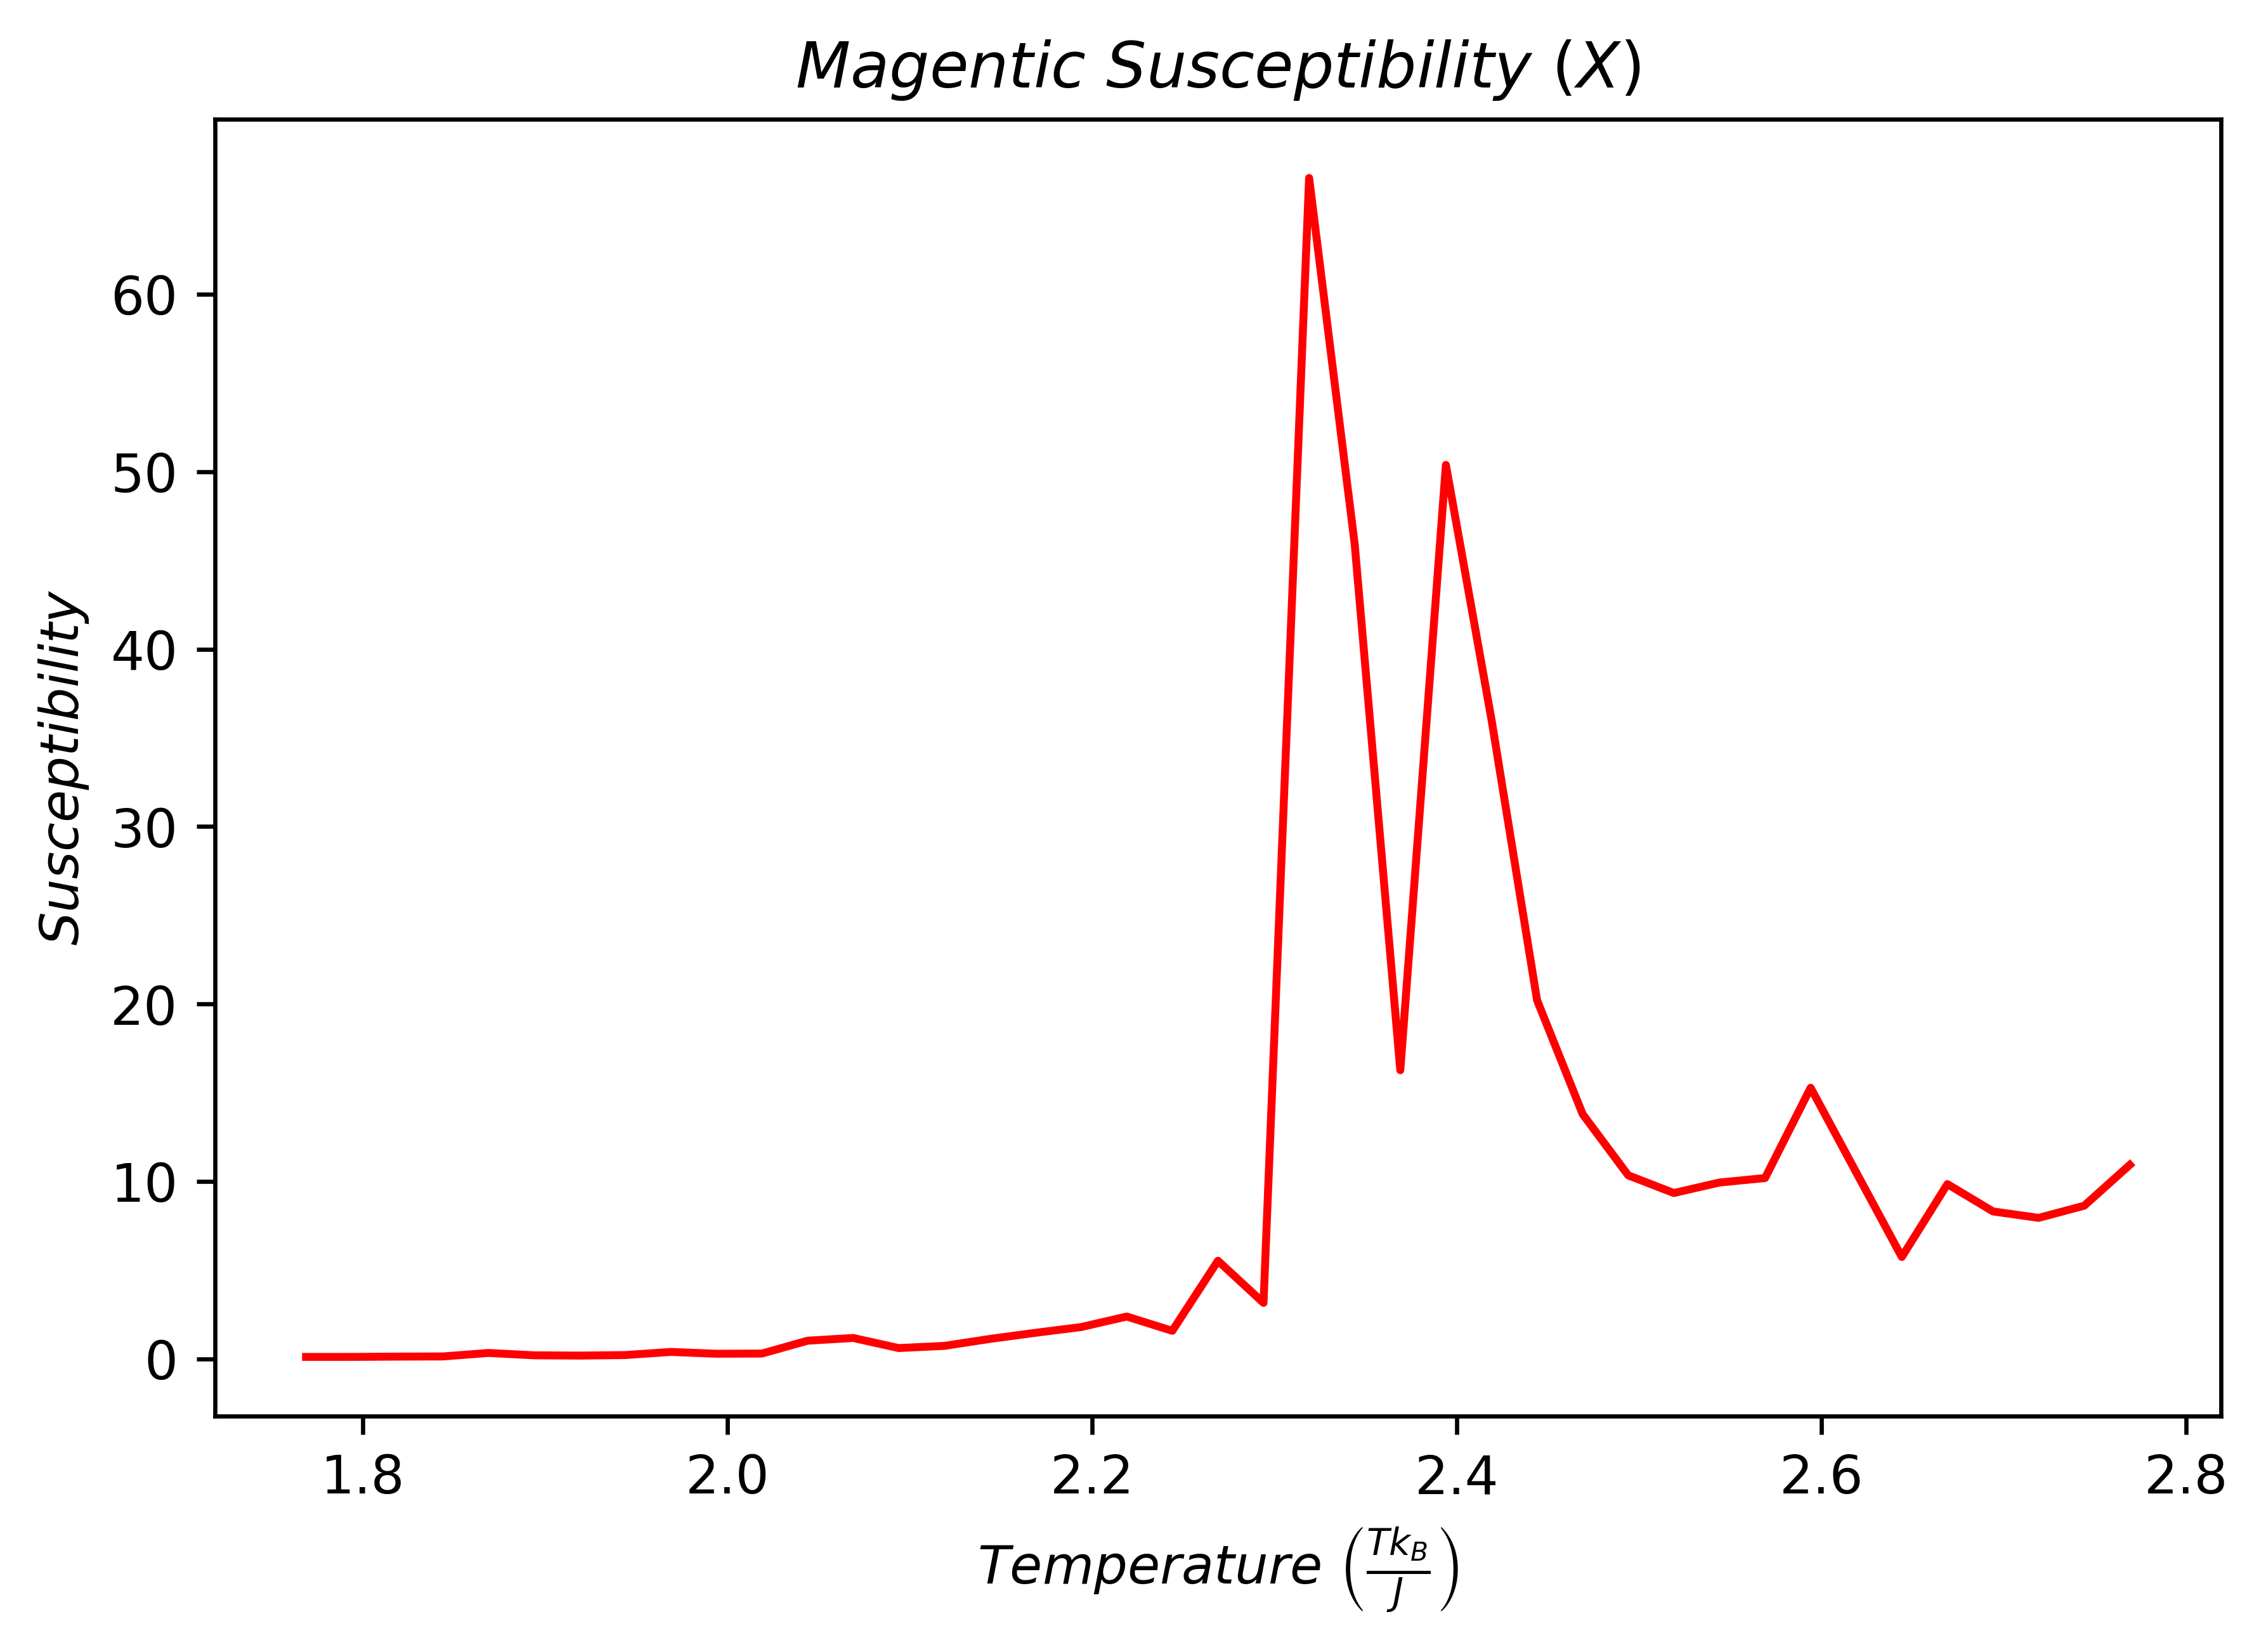
\includegraphics[scale=.45]{MagSuscept32}
\end{figure}
\begin{figure}[H]
\caption{Specific Heat Capacity for [32 X 32] lattice}
\centering
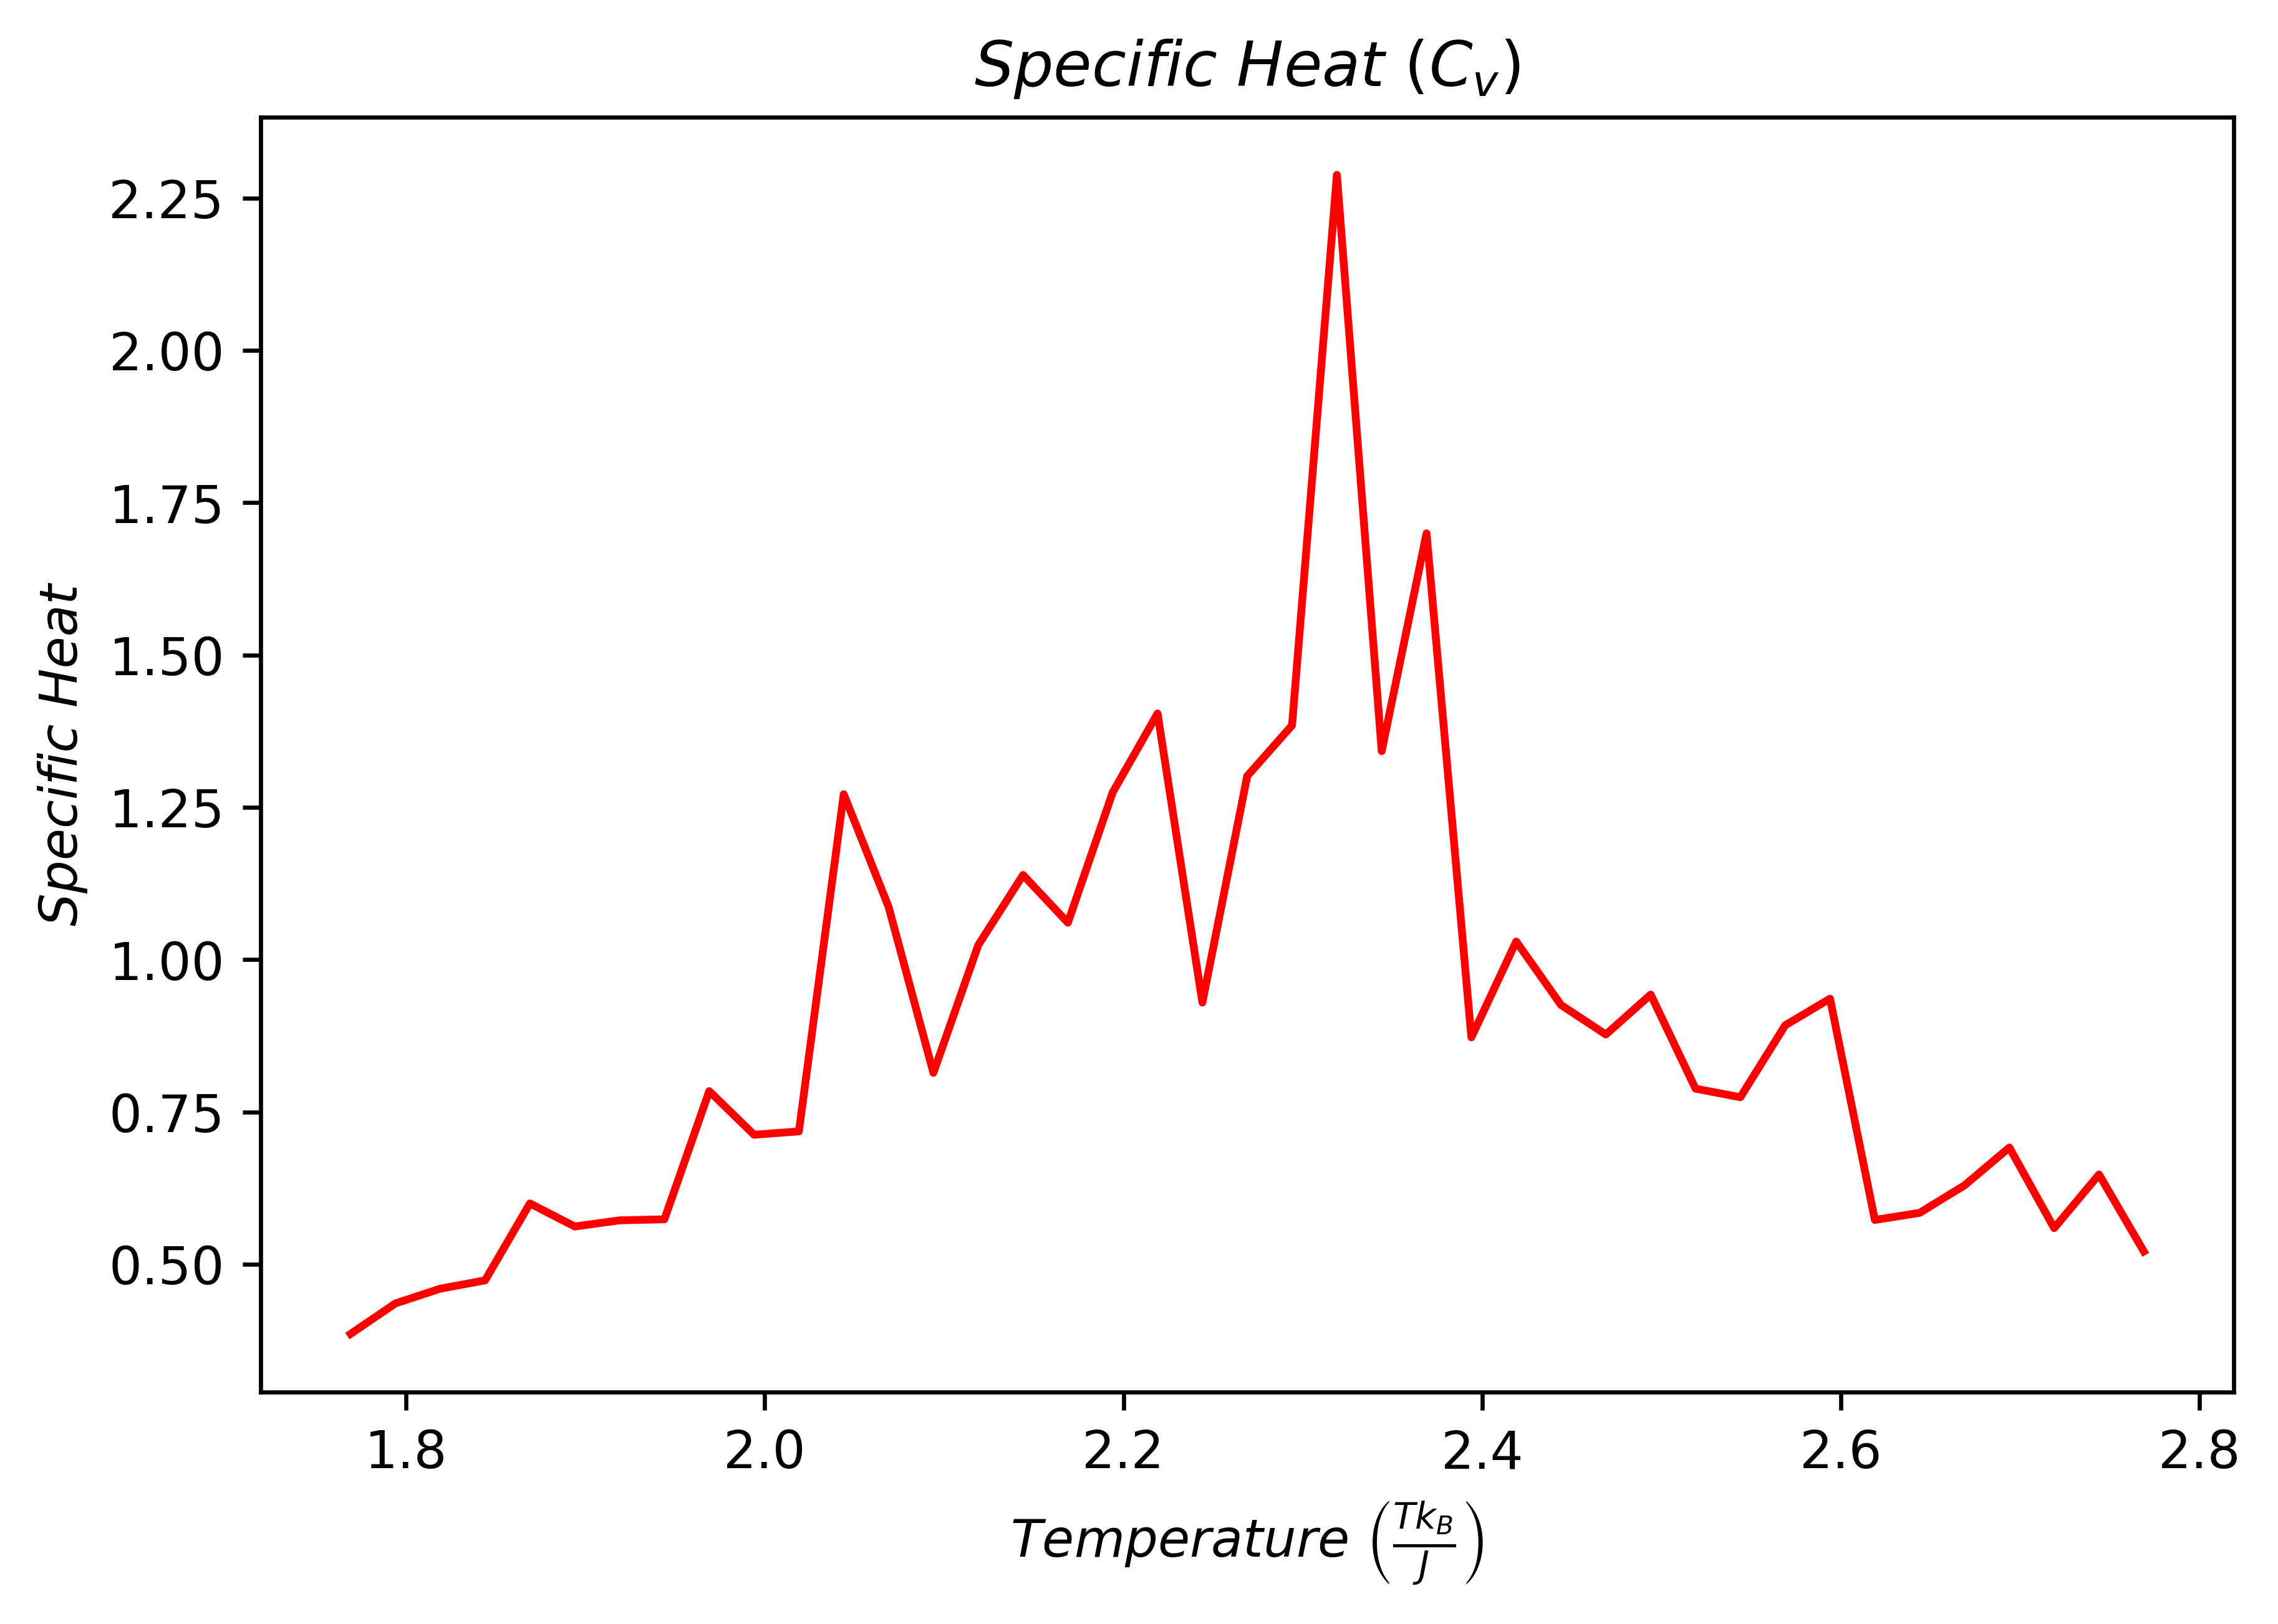
\includegraphics[scale=.45]{SpecificHeat32}
\end{figure}
%%%%%%%%%%%%%%%%%%%%%%%%%%%%%%%%%%%%%%%%%%%%%%%%%%%%%%%%%%%%
The second lattice, which was [64 X 64], proved to be very much like the [32 X 32] lattice. Both exhibited the same peaks for the specific heat capacity per spin and the magnetic susceptibility per spin about $T_c$ as seen in Figures (19) and (20). Notably, the entire evolution of specific heat plot smoothed out which is what should predictably happen as the finite size of the lattice tends towards infinity. However, the susceptibility plot became much more jagged and its peak was also quite lower, despite maintaining the same overall shape as the smaller lattice.
%%%%%%%%%%%%%%%%%%%%%%%%%%%%%%%%%%%%%%%%%%%%%%%%%%%%%%%%%%%%
\begin{figure}[H]
\caption{Magnetic Susceptibility for [64 X 64] lattice}
\centering
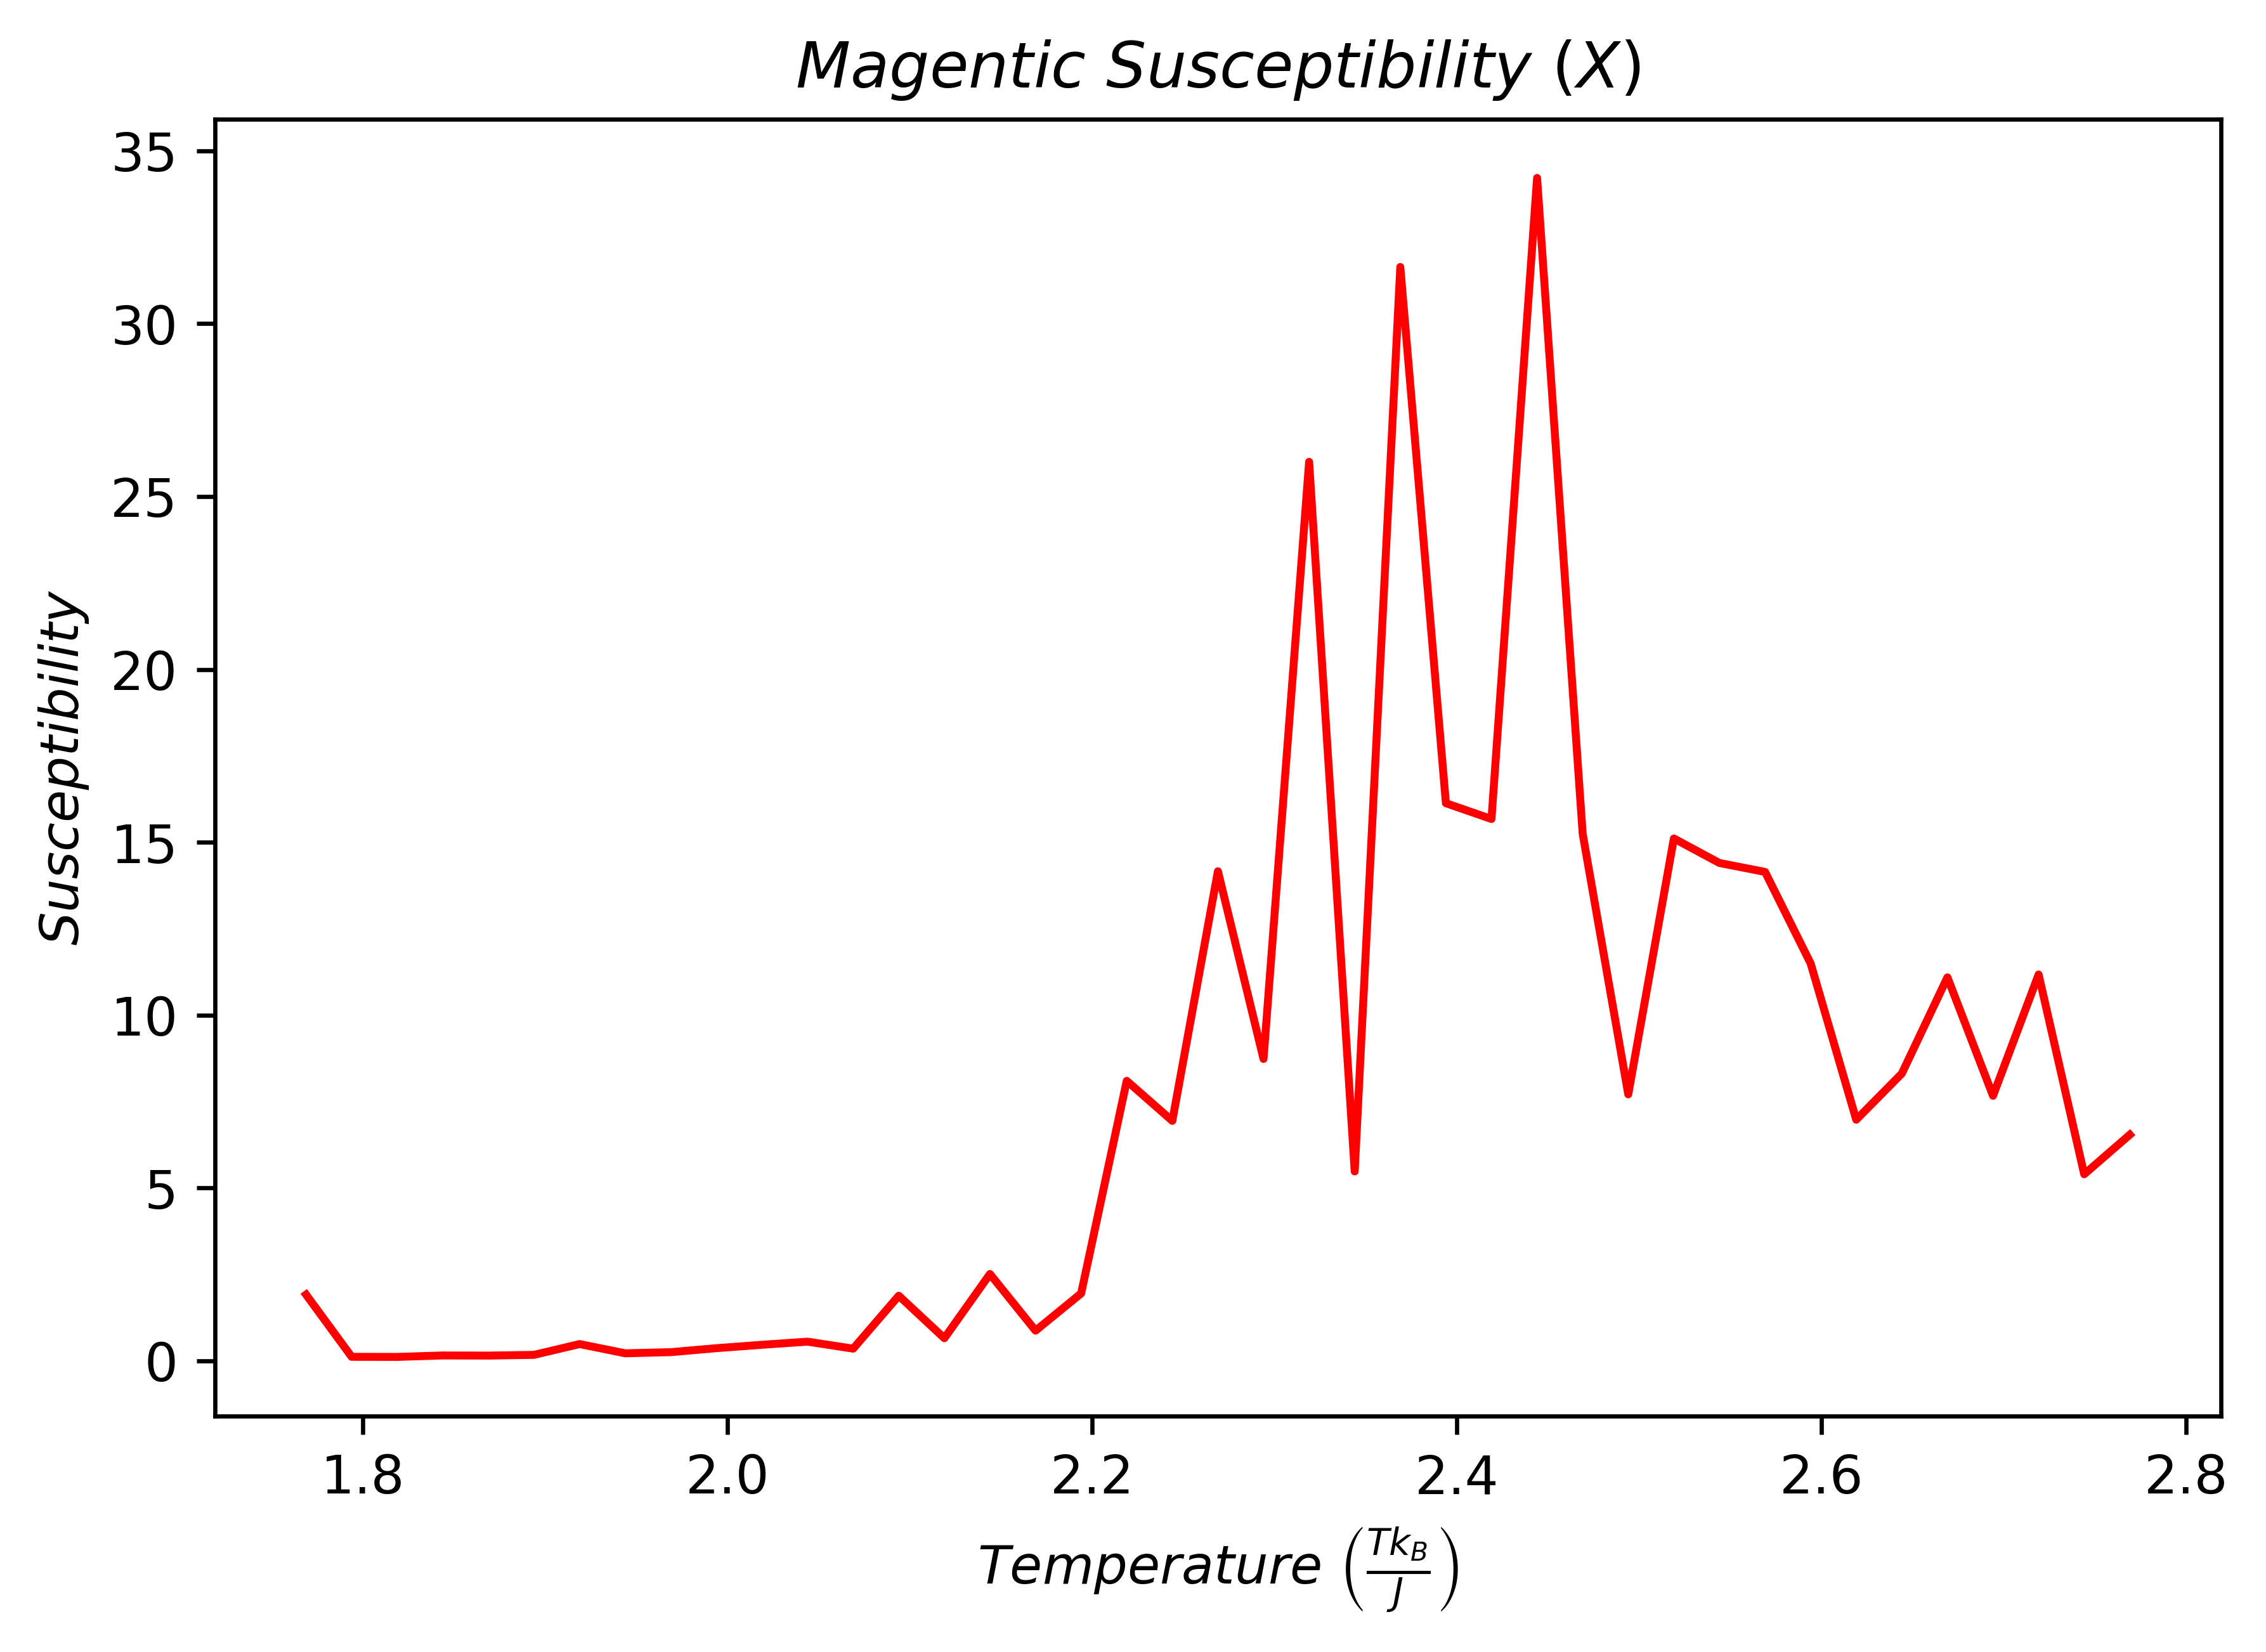
\includegraphics[scale=.45]{MagSuscept64}
\end{figure}
\begin{figure}[h]
\caption{Specific Heat Capacity for [64 X 64] lattice}
\centering
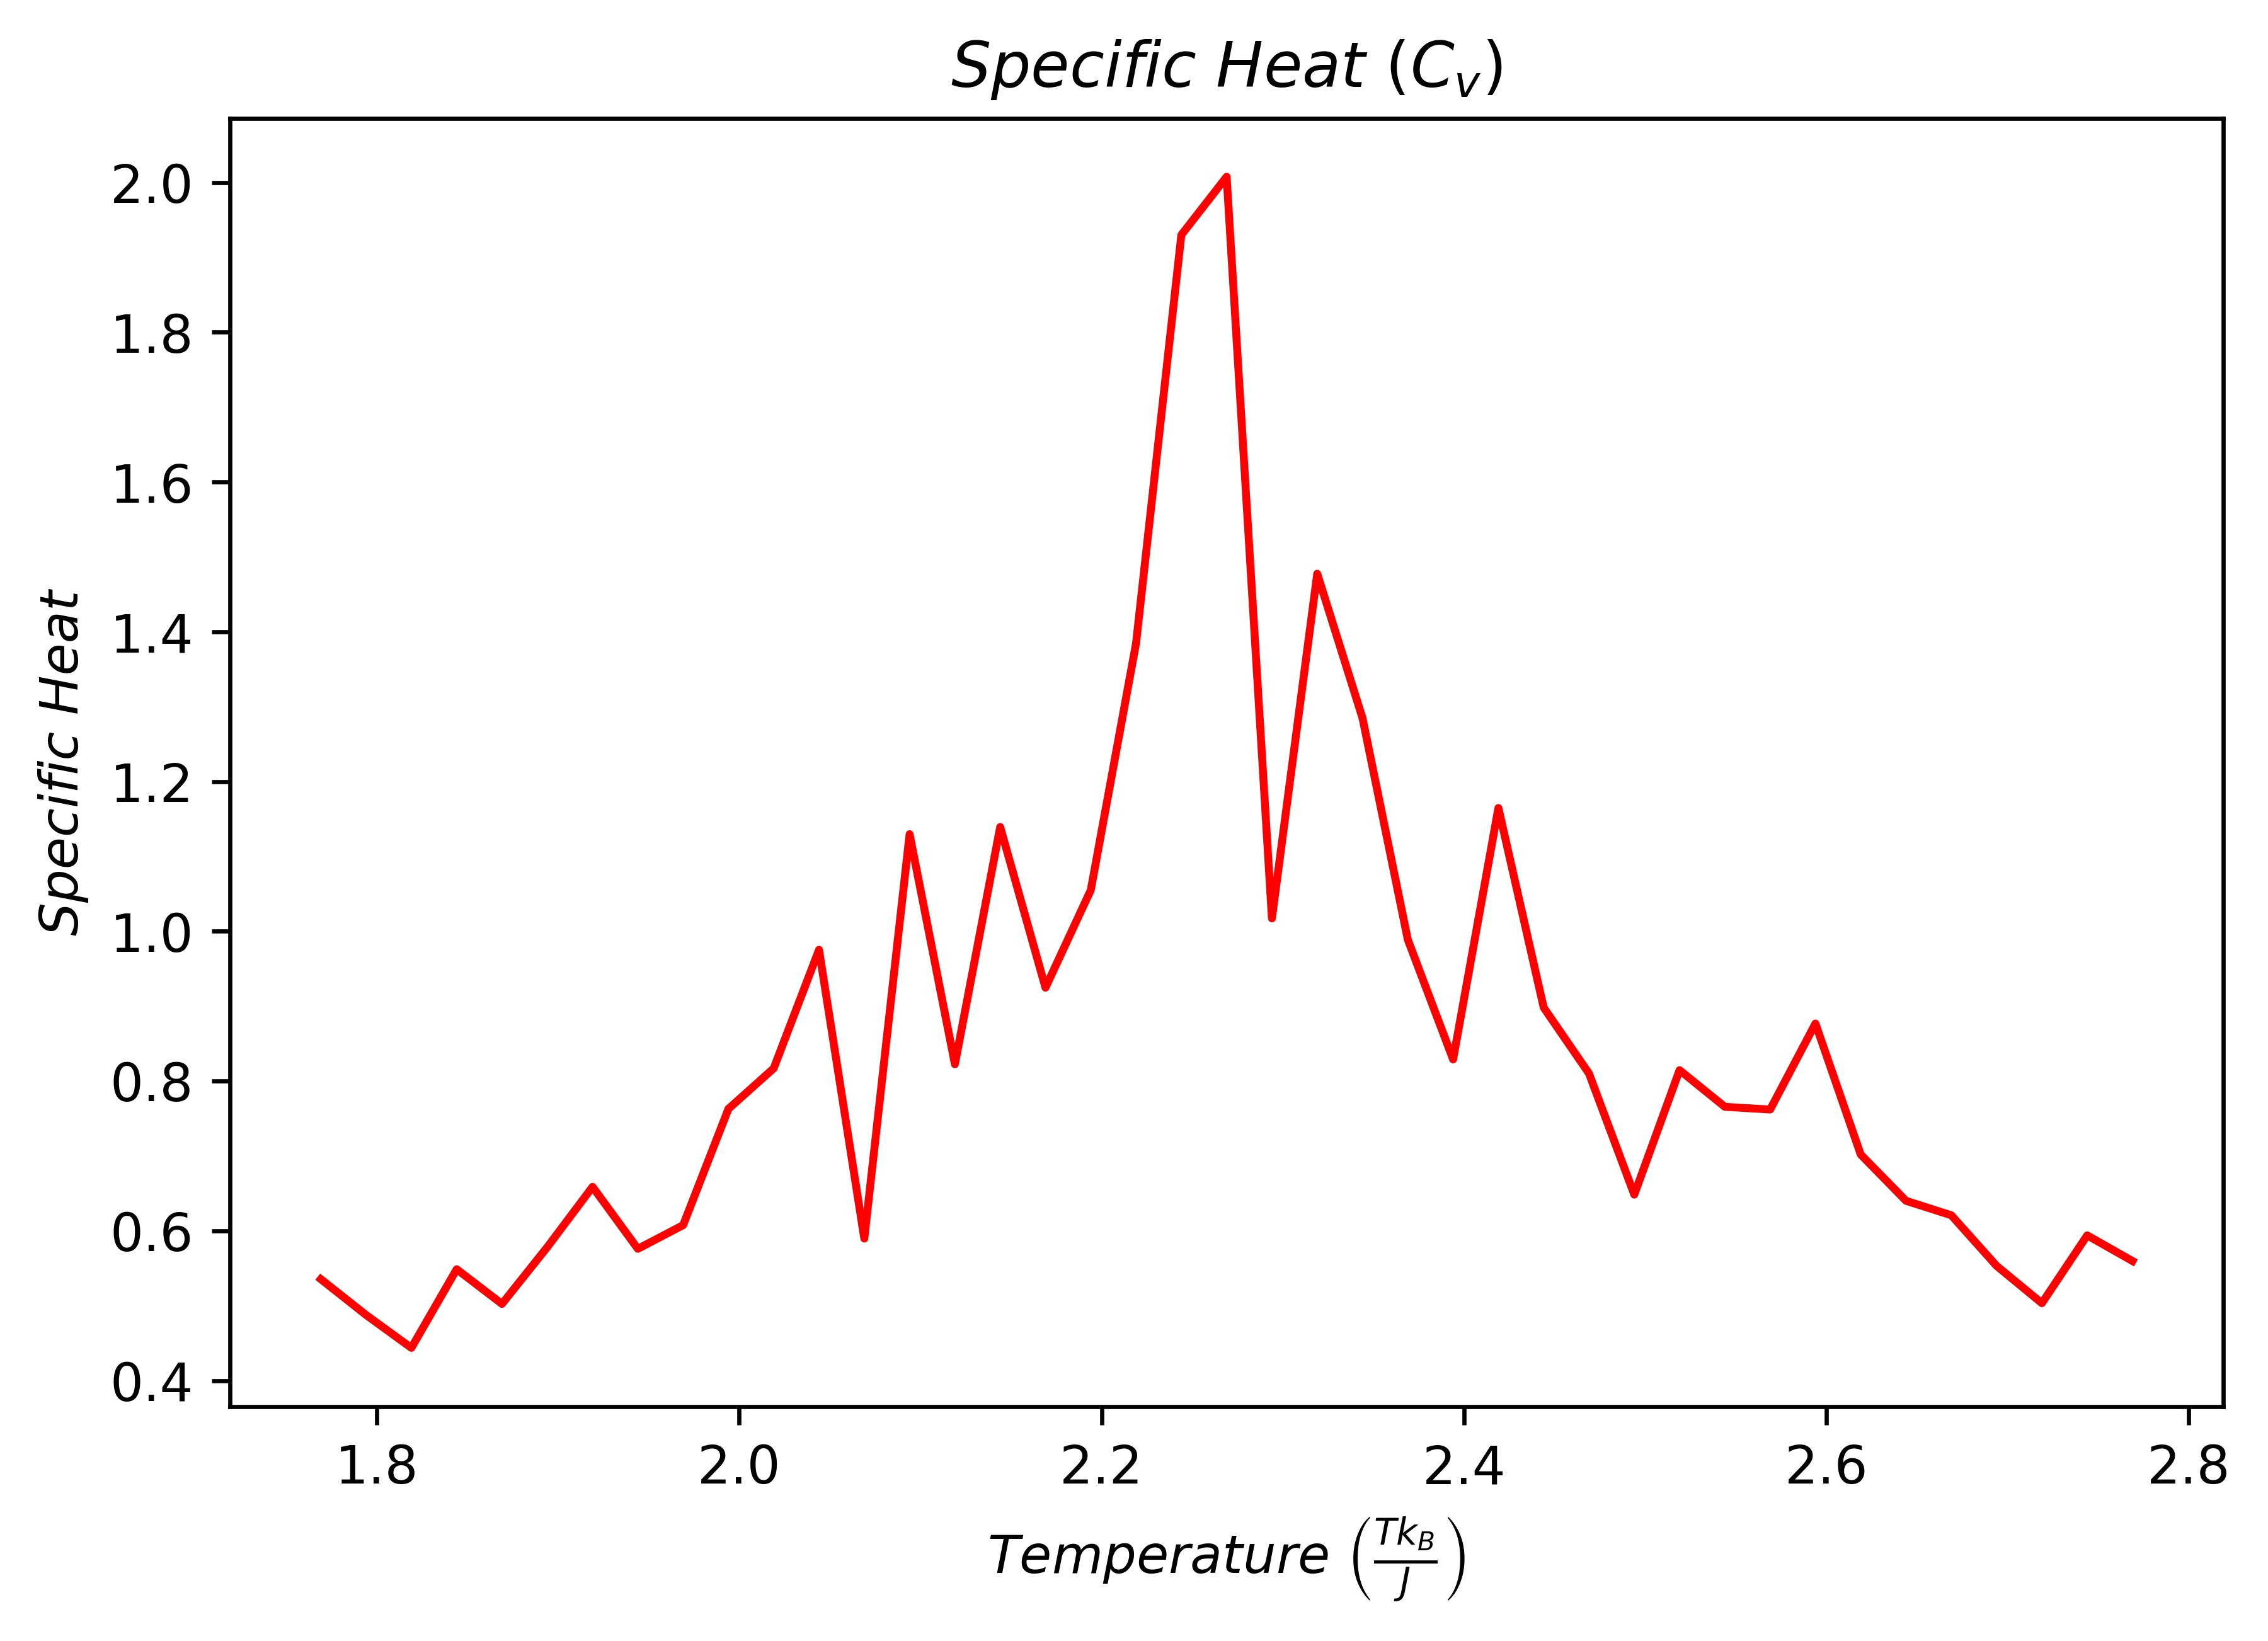
\includegraphics[scale=.45]{SpecificHeat64}
\end{figure}
%%%%%%%%%%%%%%%%%%%%%%%%%%%%%%%%%%%%%%%%%%%%%%%%%%%%%%%%%%%%
The third lattice, which was [128 X 128], proved to actually resemble the plots from the first lattice rather than the second, which is odd because the assumption being made is that as the lattice tends towards infinite size the divergence about $T_c$ should become more apparent. This is not what happened though, as Figure (21) - which plots the magnetic susceptibility - had the same two peaks that the smallest lattice had, and had a similar peak value. The plot of the specific heat capacity, however, closely followed both of the previous lattices in structure. Figure (22) does reveal that it has a strange peak at the very beginning of structure but this is more than likely due to odd initial configuration as the lattice begins randomly aligned. 
%%%%%%%%%%%%%%%%%%%%%%%%%%%%%%%%%%%%%%%%%%%%%%%%%%%%%%%%%%%%
\begin{figure}[H]
\caption{Magnetic Susceptibility for [128 X 128 lattice}
\centering
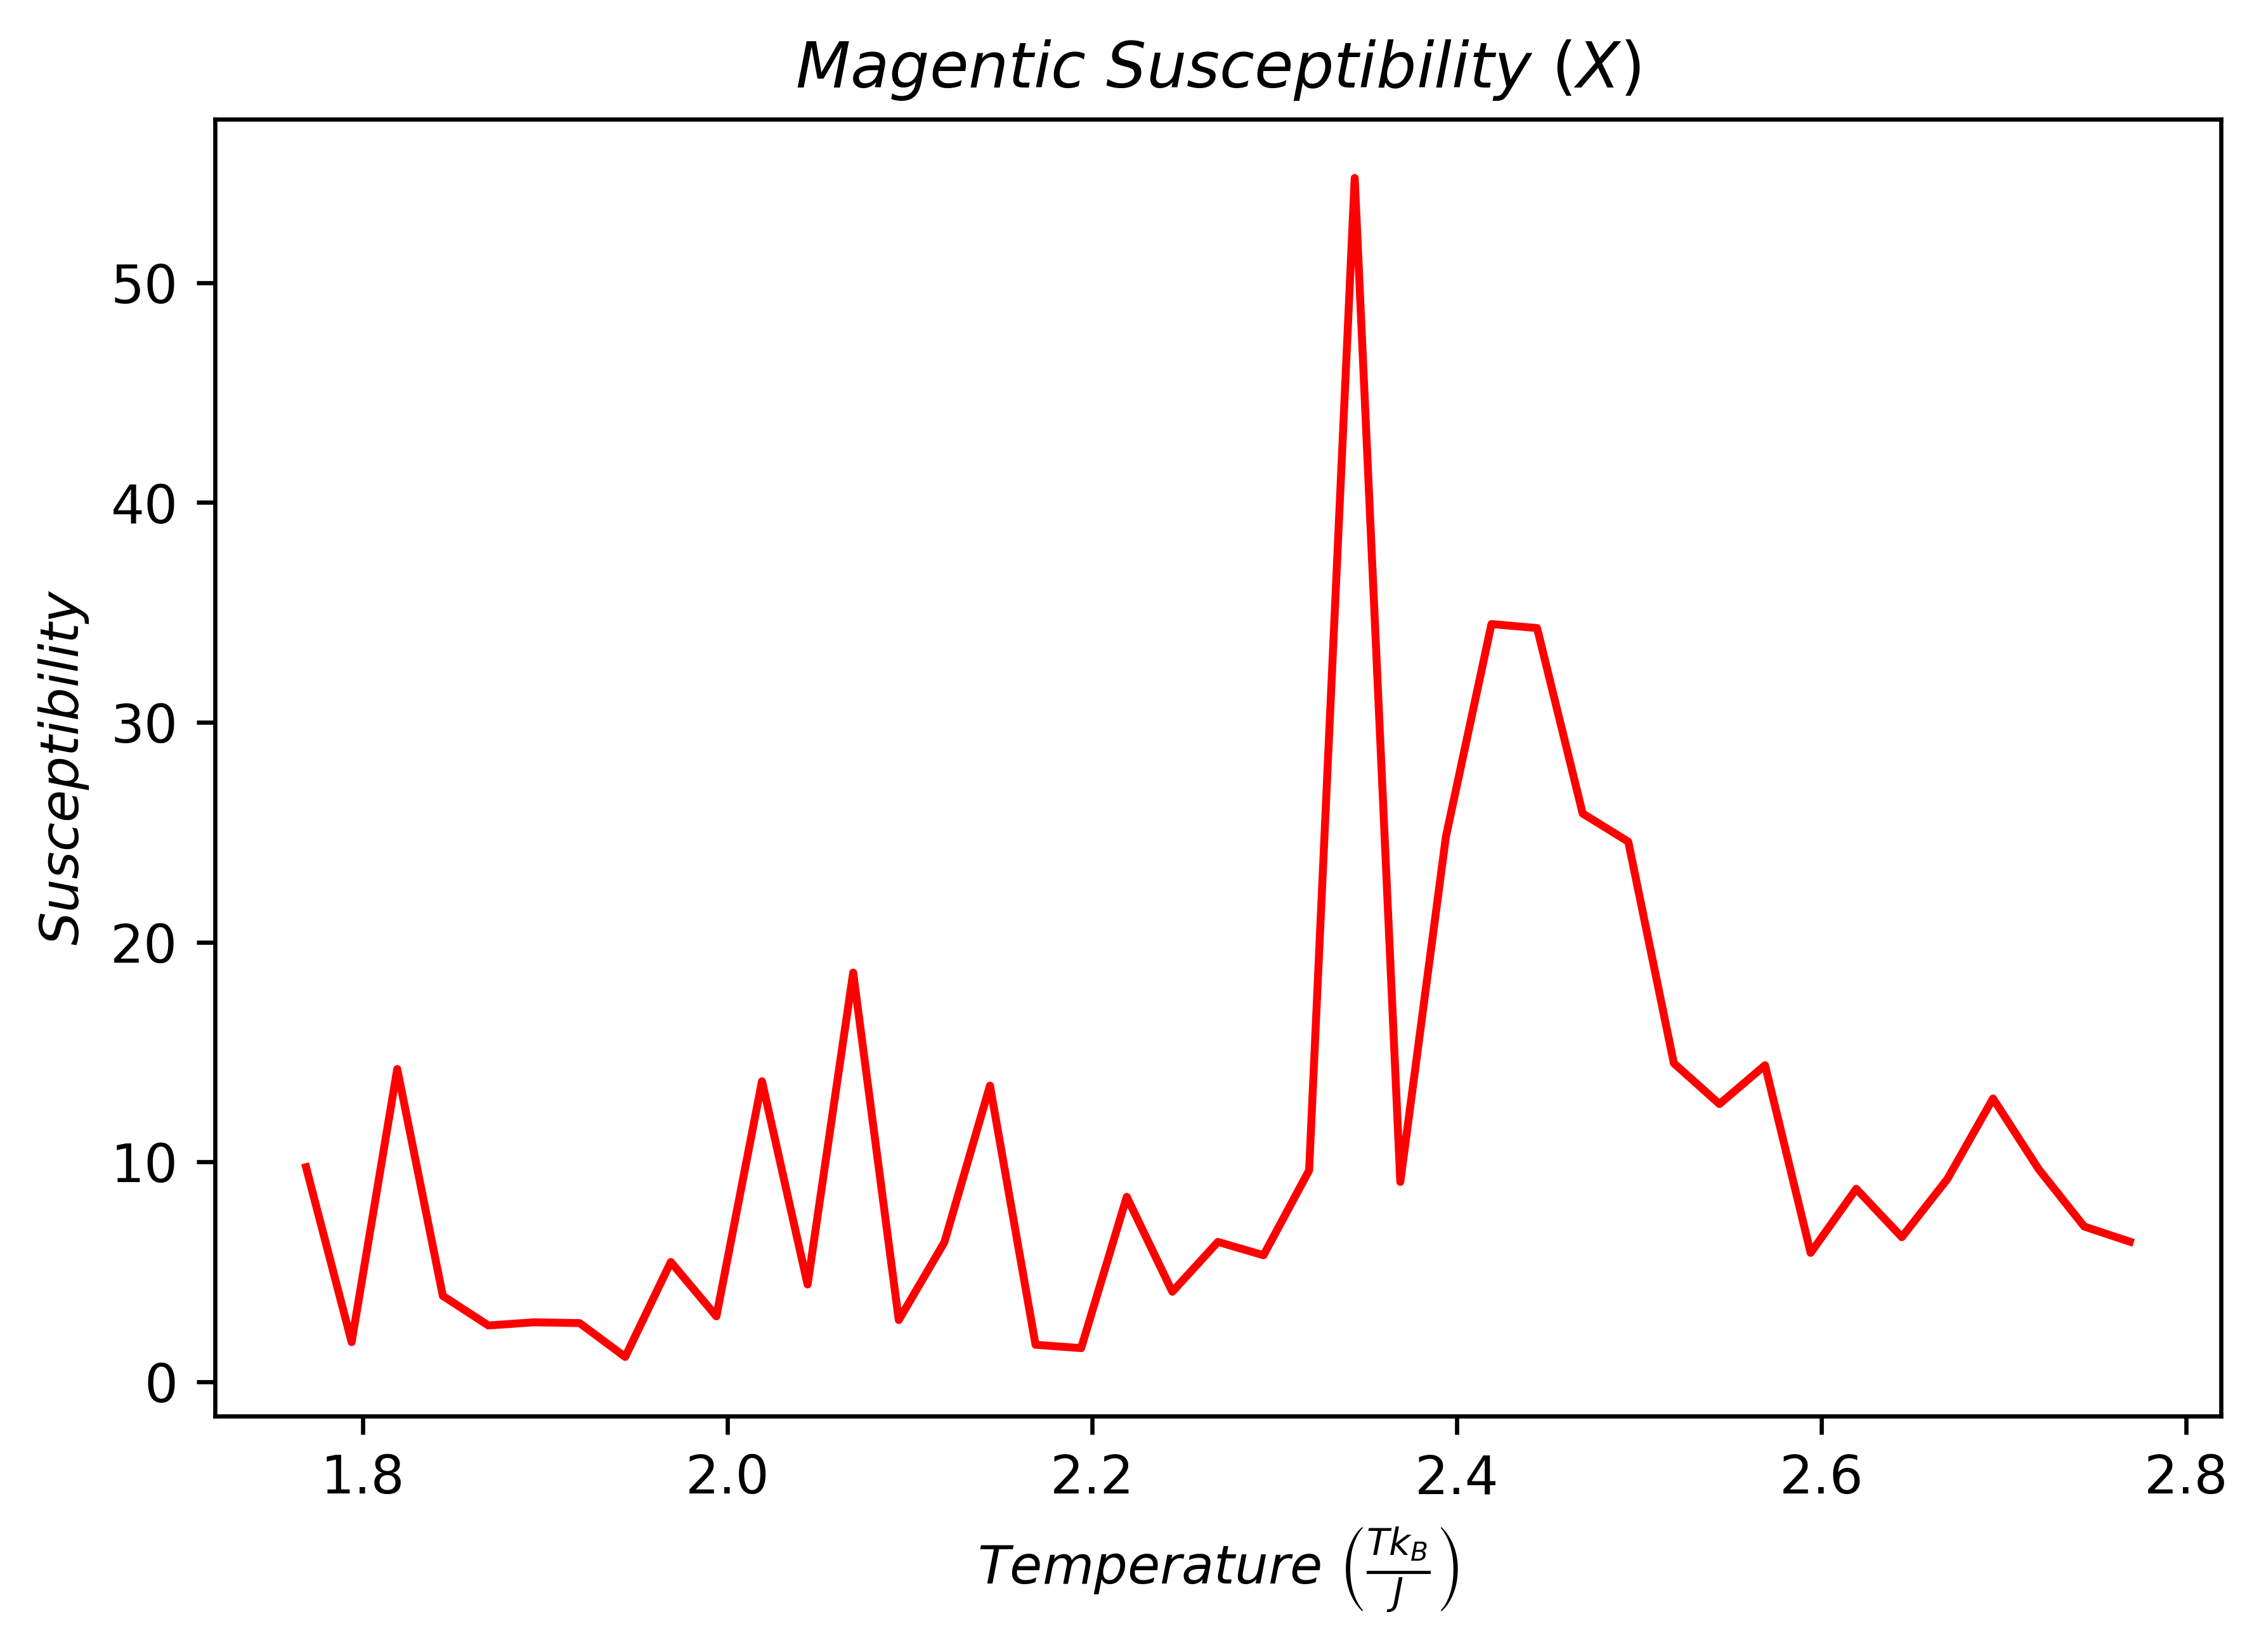
\includegraphics[scale=.45]{MagSuscept128}
\end{figure}
\begin{figure}[h]
\caption{Specific Heat Capacity for [128 X 128 lattice}
\centering
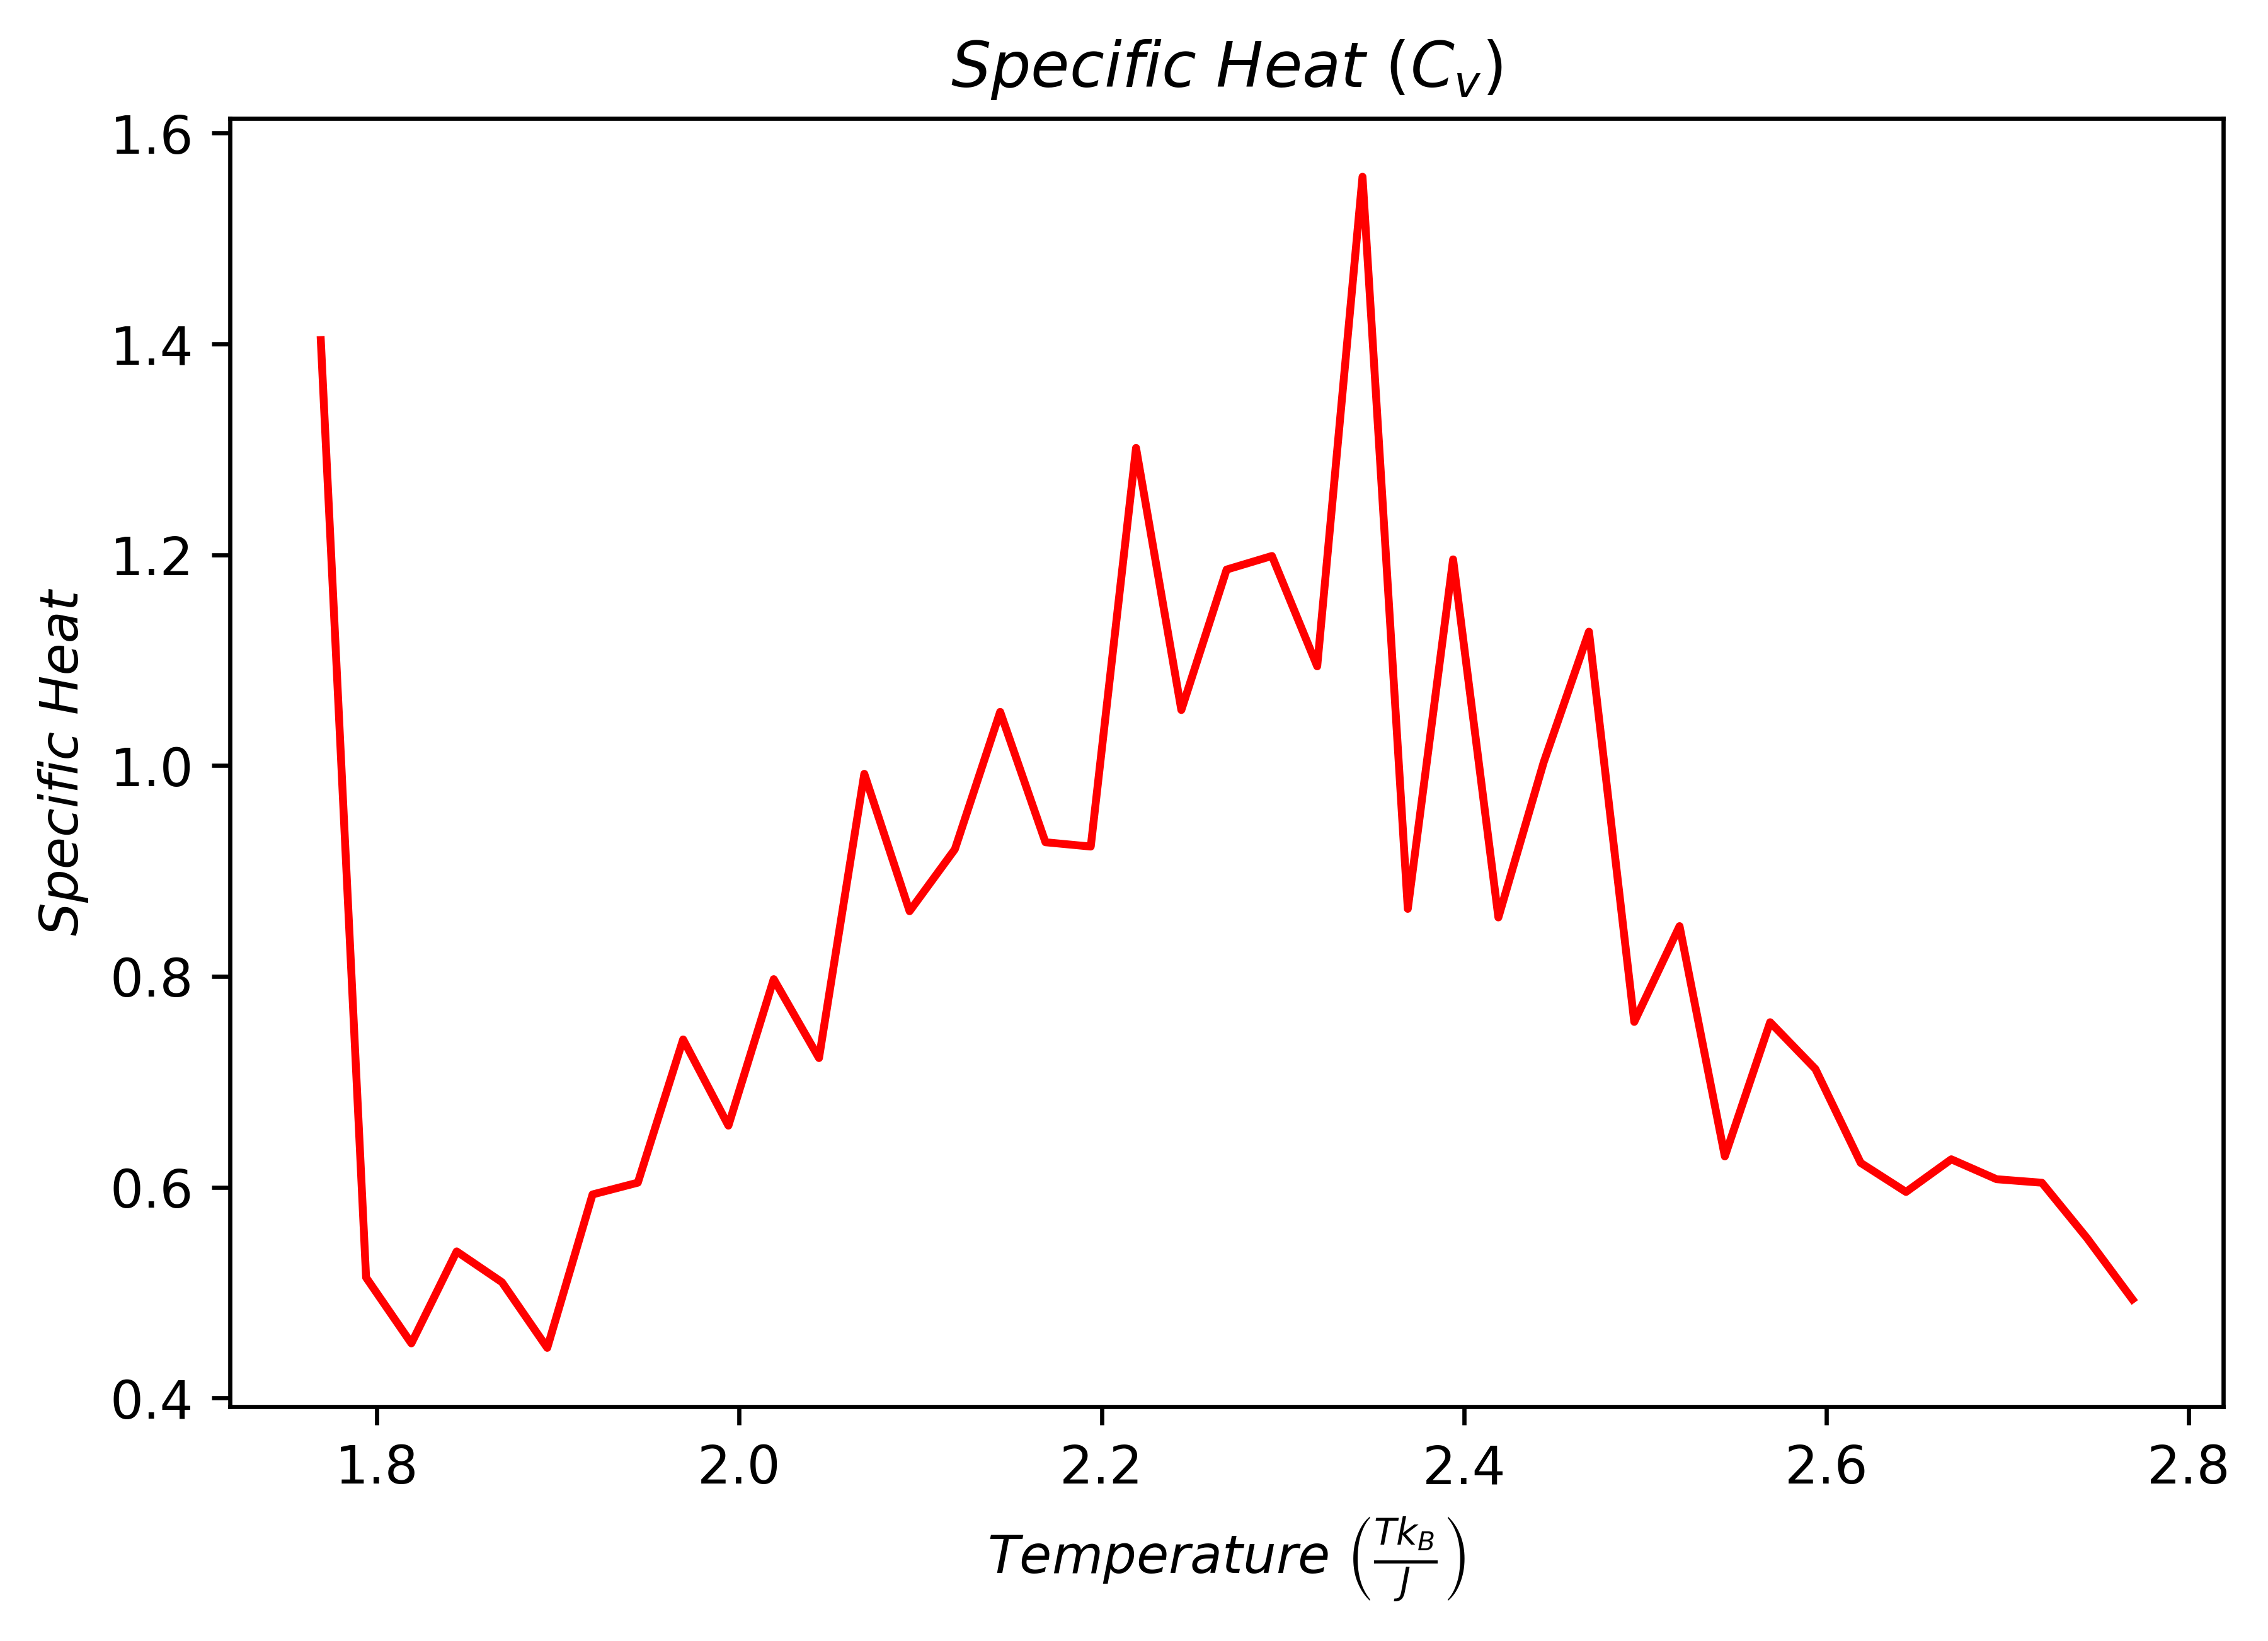
\includegraphics[scale=.45]{SpecificHeat128}
\end{figure}
%%%%%%%%%%%%%%%%%%%%%%%%%%%%%%%%%%%%%%%%%%%%%%%%%%%%%%%%%%%%
The final lattice, which was [256 X 256], was oddly enough the strangest of them all. Its magnetic susceptibility varied wildly just before and after the critical temperature indicating that something peculiar was going on as seen in Figure (23). That said the sharpest peak still occurred at the critical temperature which was the goal to observe. The specific heat capacity on the other hand, displayed the same structure as the rest of the lattices: a peak at the critical temperature, and descending values around it. It should certainly be noted that the initial tail seen at $T=1.8$ in Figure (24) is again due to the initial configuration of the lattice, since many of its Monte-Carlo sweeps would be recording skewed data. If this theory holds true, then more than likely there was not enough discarded data. That said, at the very least all of the plots displayed clear peaks about the critical temperature showing that a second order phase transition was attempting to occur if not occurring outright.
%%%%%%%%%%%%%%%%%%%%%%%%%%%%%%%%%%%%%%%%%%%%%%%%%%%%%%%%%%%%
\begin{figure}[H]
\caption{Magnetic Susceptibility for [256 X 256] lattice}
\centering
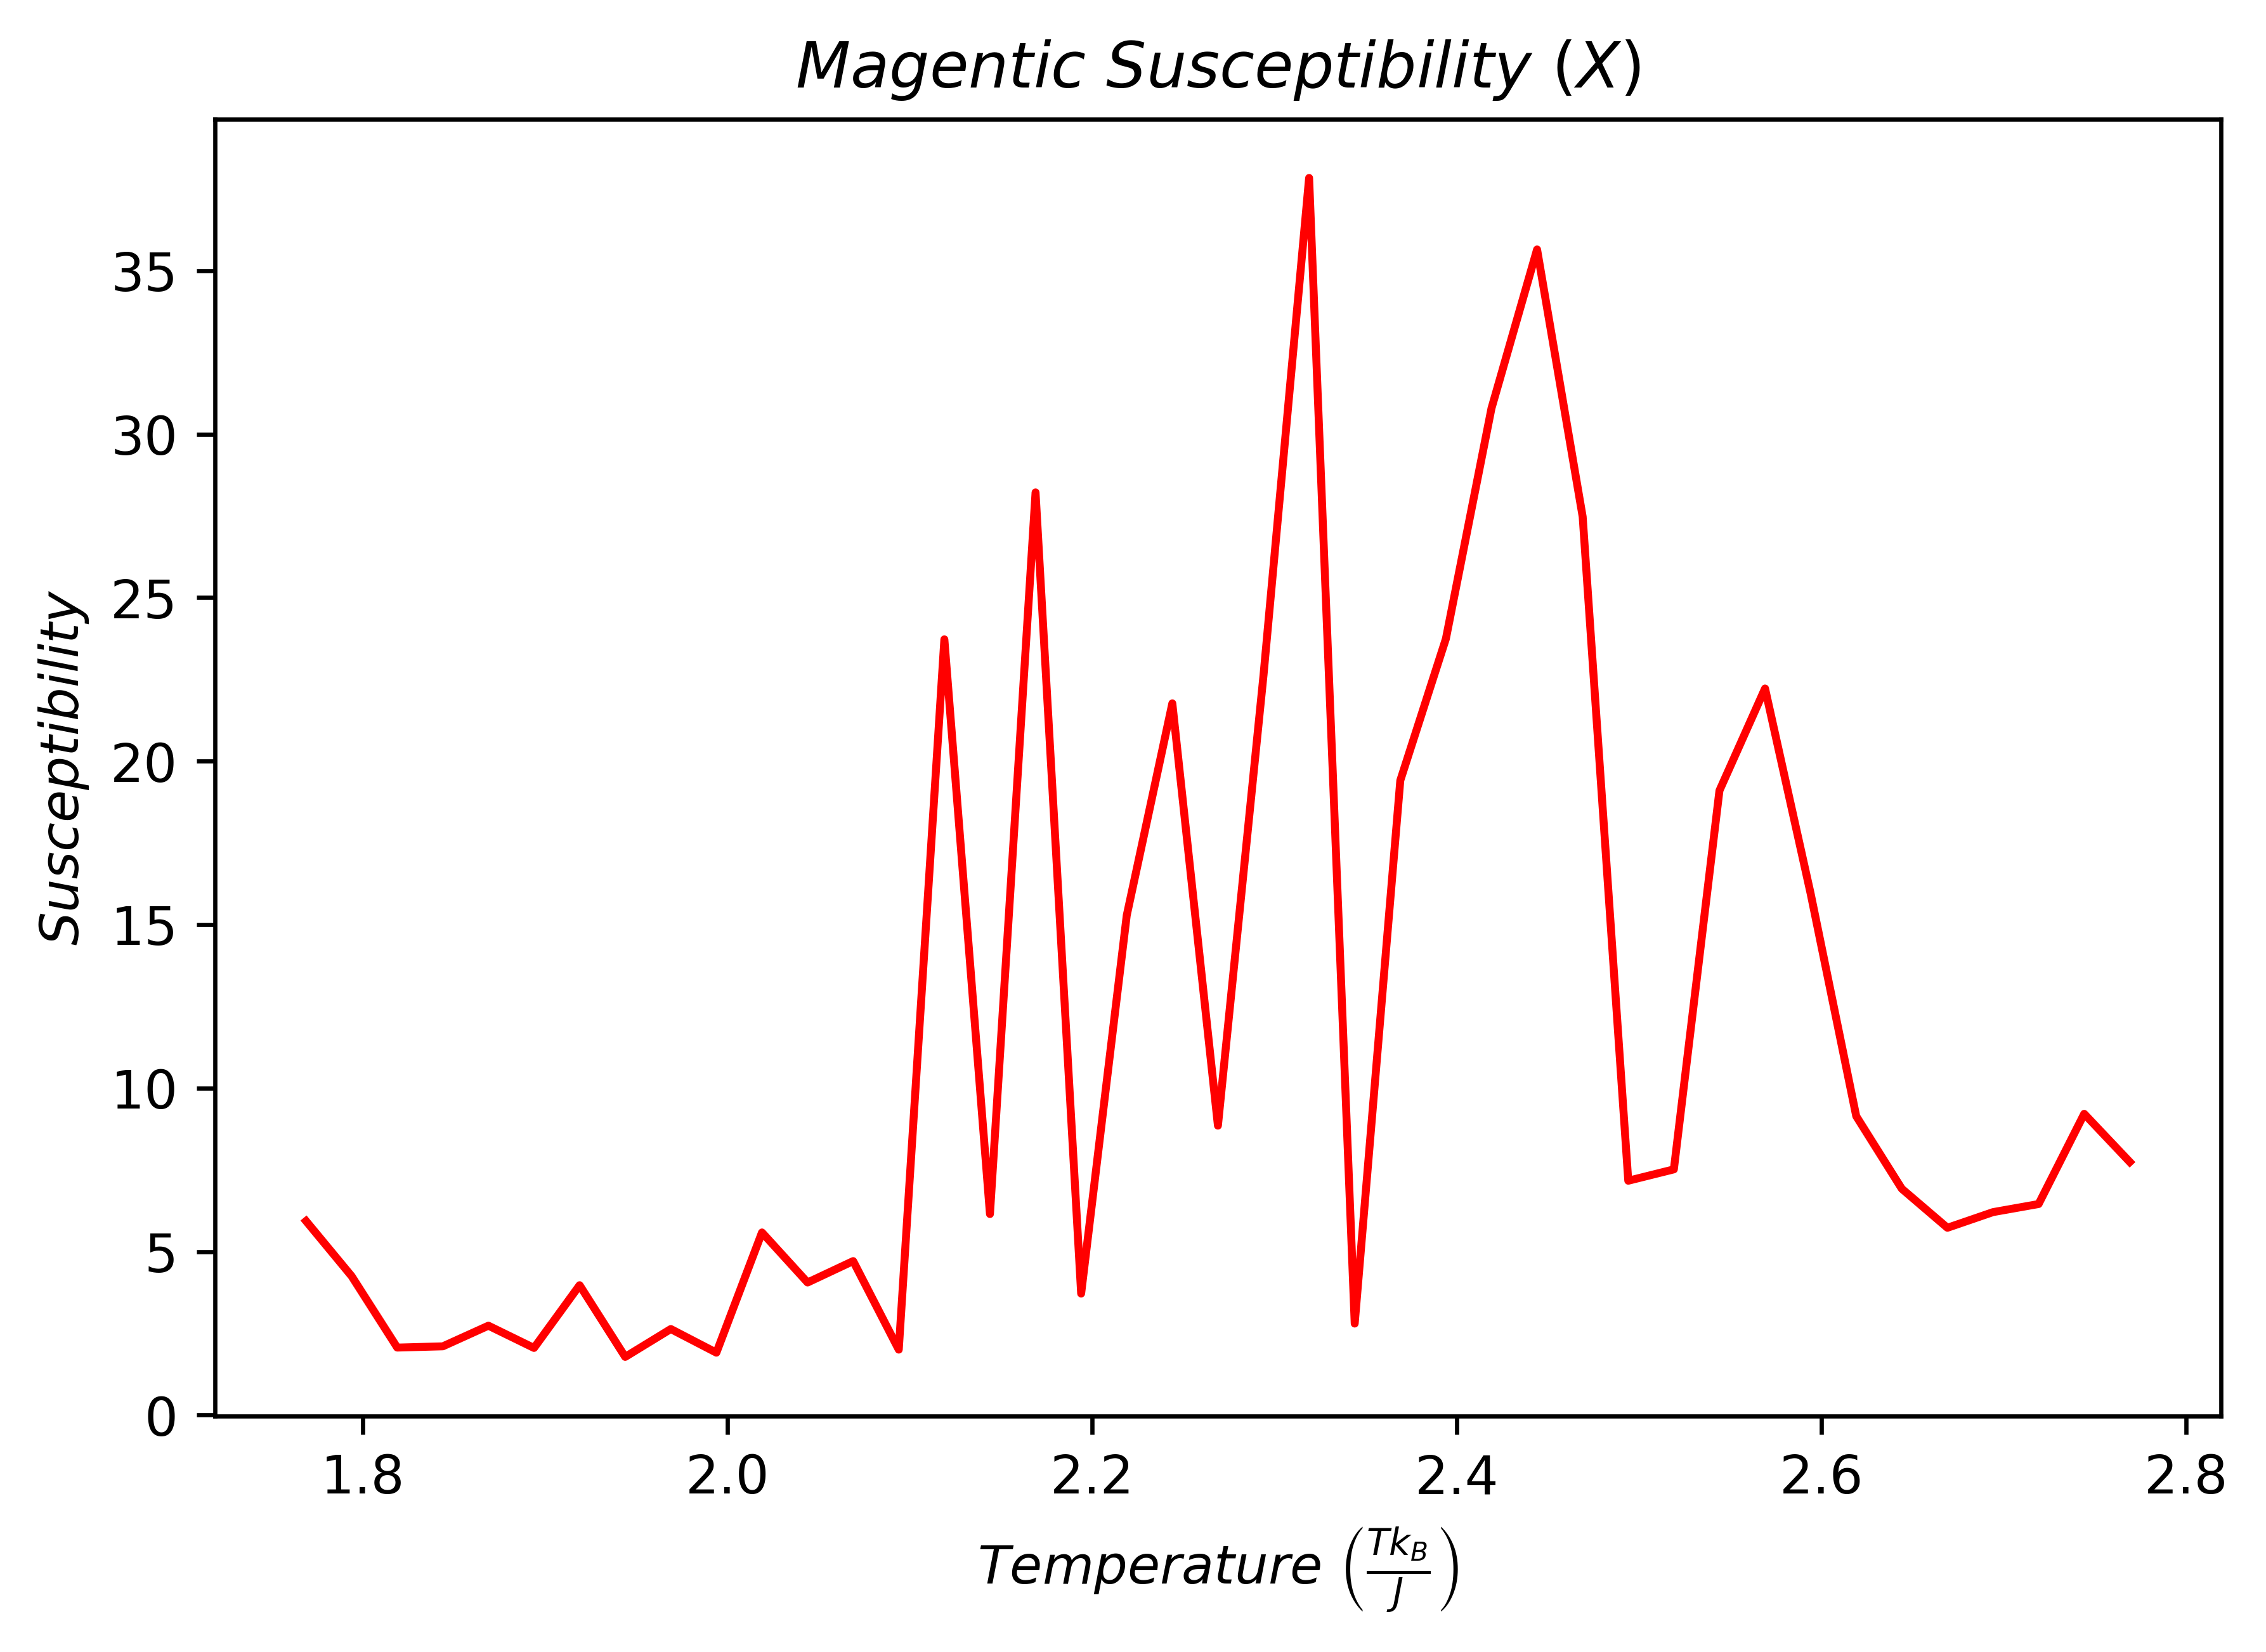
\includegraphics[scale=.45]{MagSuscept256}
\end{figure}
\begin{figure}[h]
\caption{Specific Heat Capacity for [256 X 256] lattice}
\centering
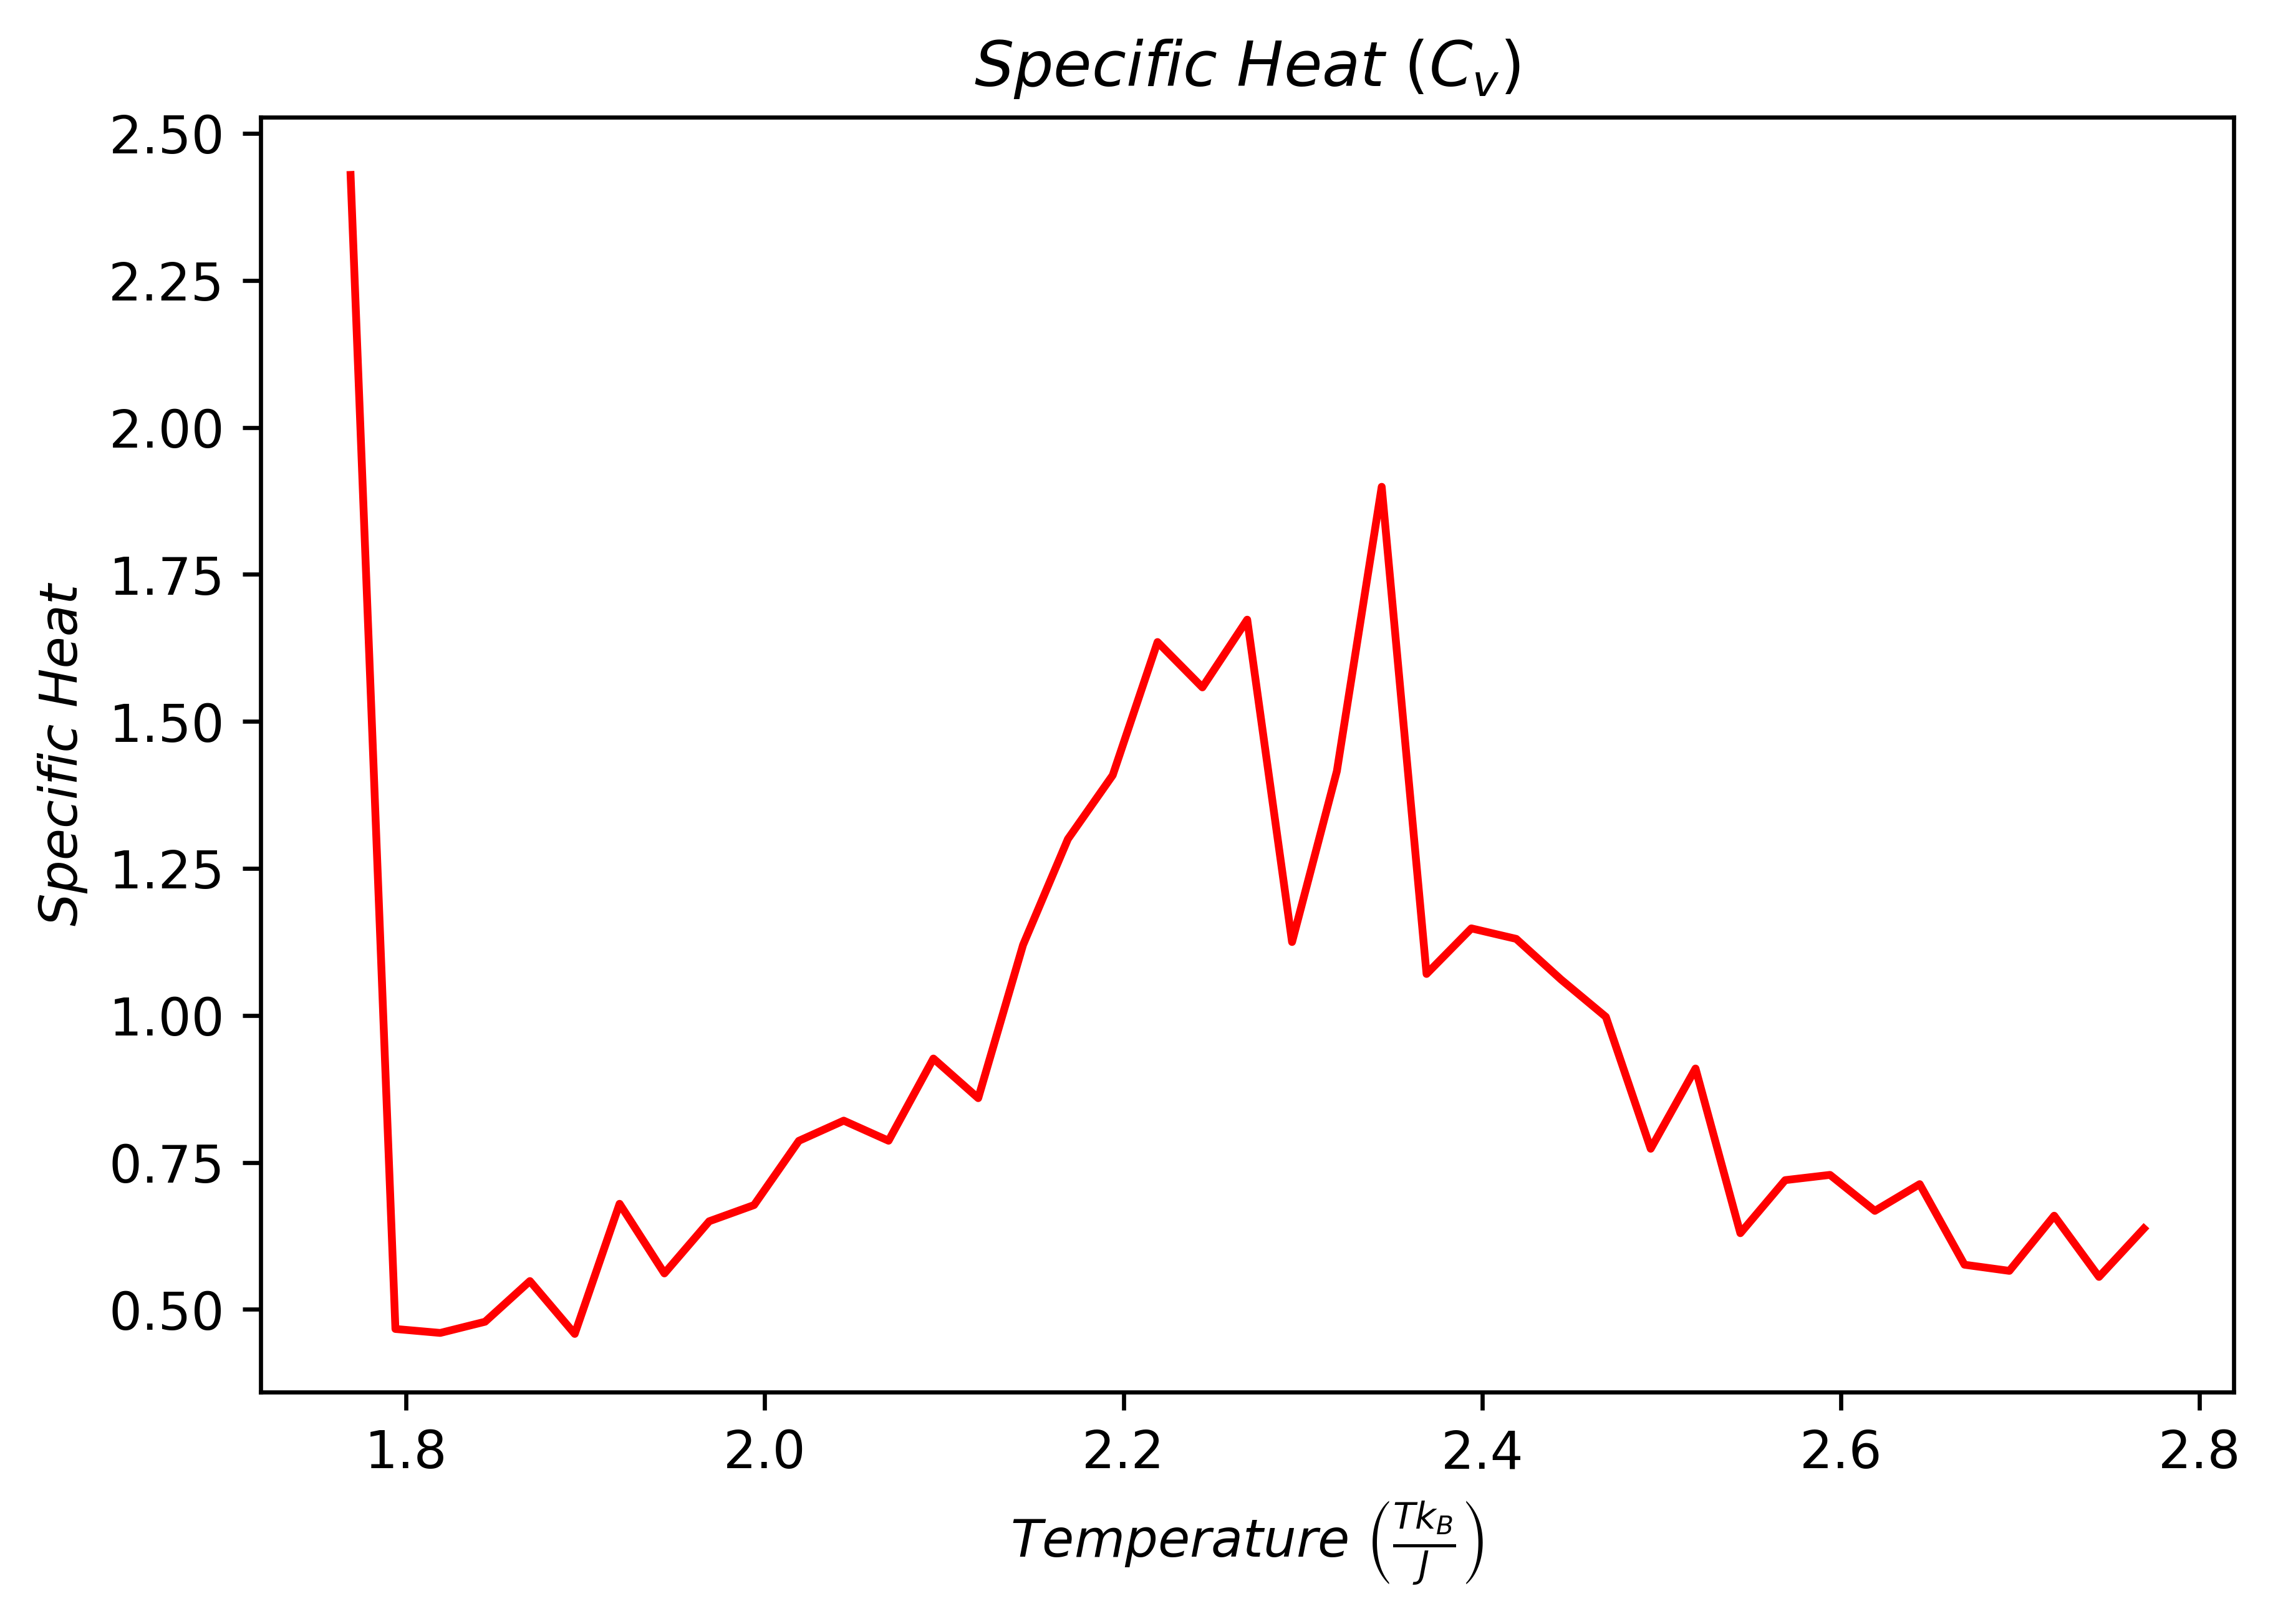
\includegraphics[scale=.45]{SpecificHeat256}
\end{figure}
%%%%%%%%%%%%%%%%%%%%%%%%%%%%%%%%%%%%%%%%%%%%%%%%%%%%%%%%%%%%
%%%%%%%%%%%%%%%%%%%%%%%%%%%%%%%%%%%
% New Section
%%%%%%%%%%%%%%%%%%%%%%%%%%%%%%%%%%%
\section{Experiment Three Analysis}
\hspace{\parindent}Experiment three was essentially the second part of experiment two except that the exchange coupling energy was flipped (i.e. $J=-1$). This flip in the exchange coupling meant that the single [128 X 128] lattice was in the anti-ferromagnetic realm rather than the ferromagnetic one that the other experiments so far had been performed in. Consequentially, new behavior was expected, and indeed revealed. Computing the temperature dependence of the specific heat capacity, magnetic susceptibility, and mean dipole magnetization showed: that the magnetic susceptibility increased gradually but consistently as the temperature increased, that the mean dipole magnetization fluctuated about zero irregardless of the temperature, and that the specific heat capacity maintained a similar shape to that found in part two of experiment two, even going so far as to peak at the critical temperature. These behaviors as seen in Figures (25), (26), and (27), show that despite the change in the nature of the lattice (i.e. changing from ferromagnetic to anti-ferromagnetic) its specific heat capacity remained largely the same suggesting that it still undergoes a second order phase transition at the critical temperature where a continuous antiferromagnetic-paramagnetic phase transition is known to occur. \\
%%%%%%%%%%%%%%%%%%%%%%%%%%%%%%%%%%%%%%%%%%%%%%%%%%%%%%%%%%%%
\begin{figure}[H]
\caption{Magnetic Susceptibility for the anti-ferromagnetic lattice. Here the susceptibility is shown to increase as response to the temperature increasing.}
\centering
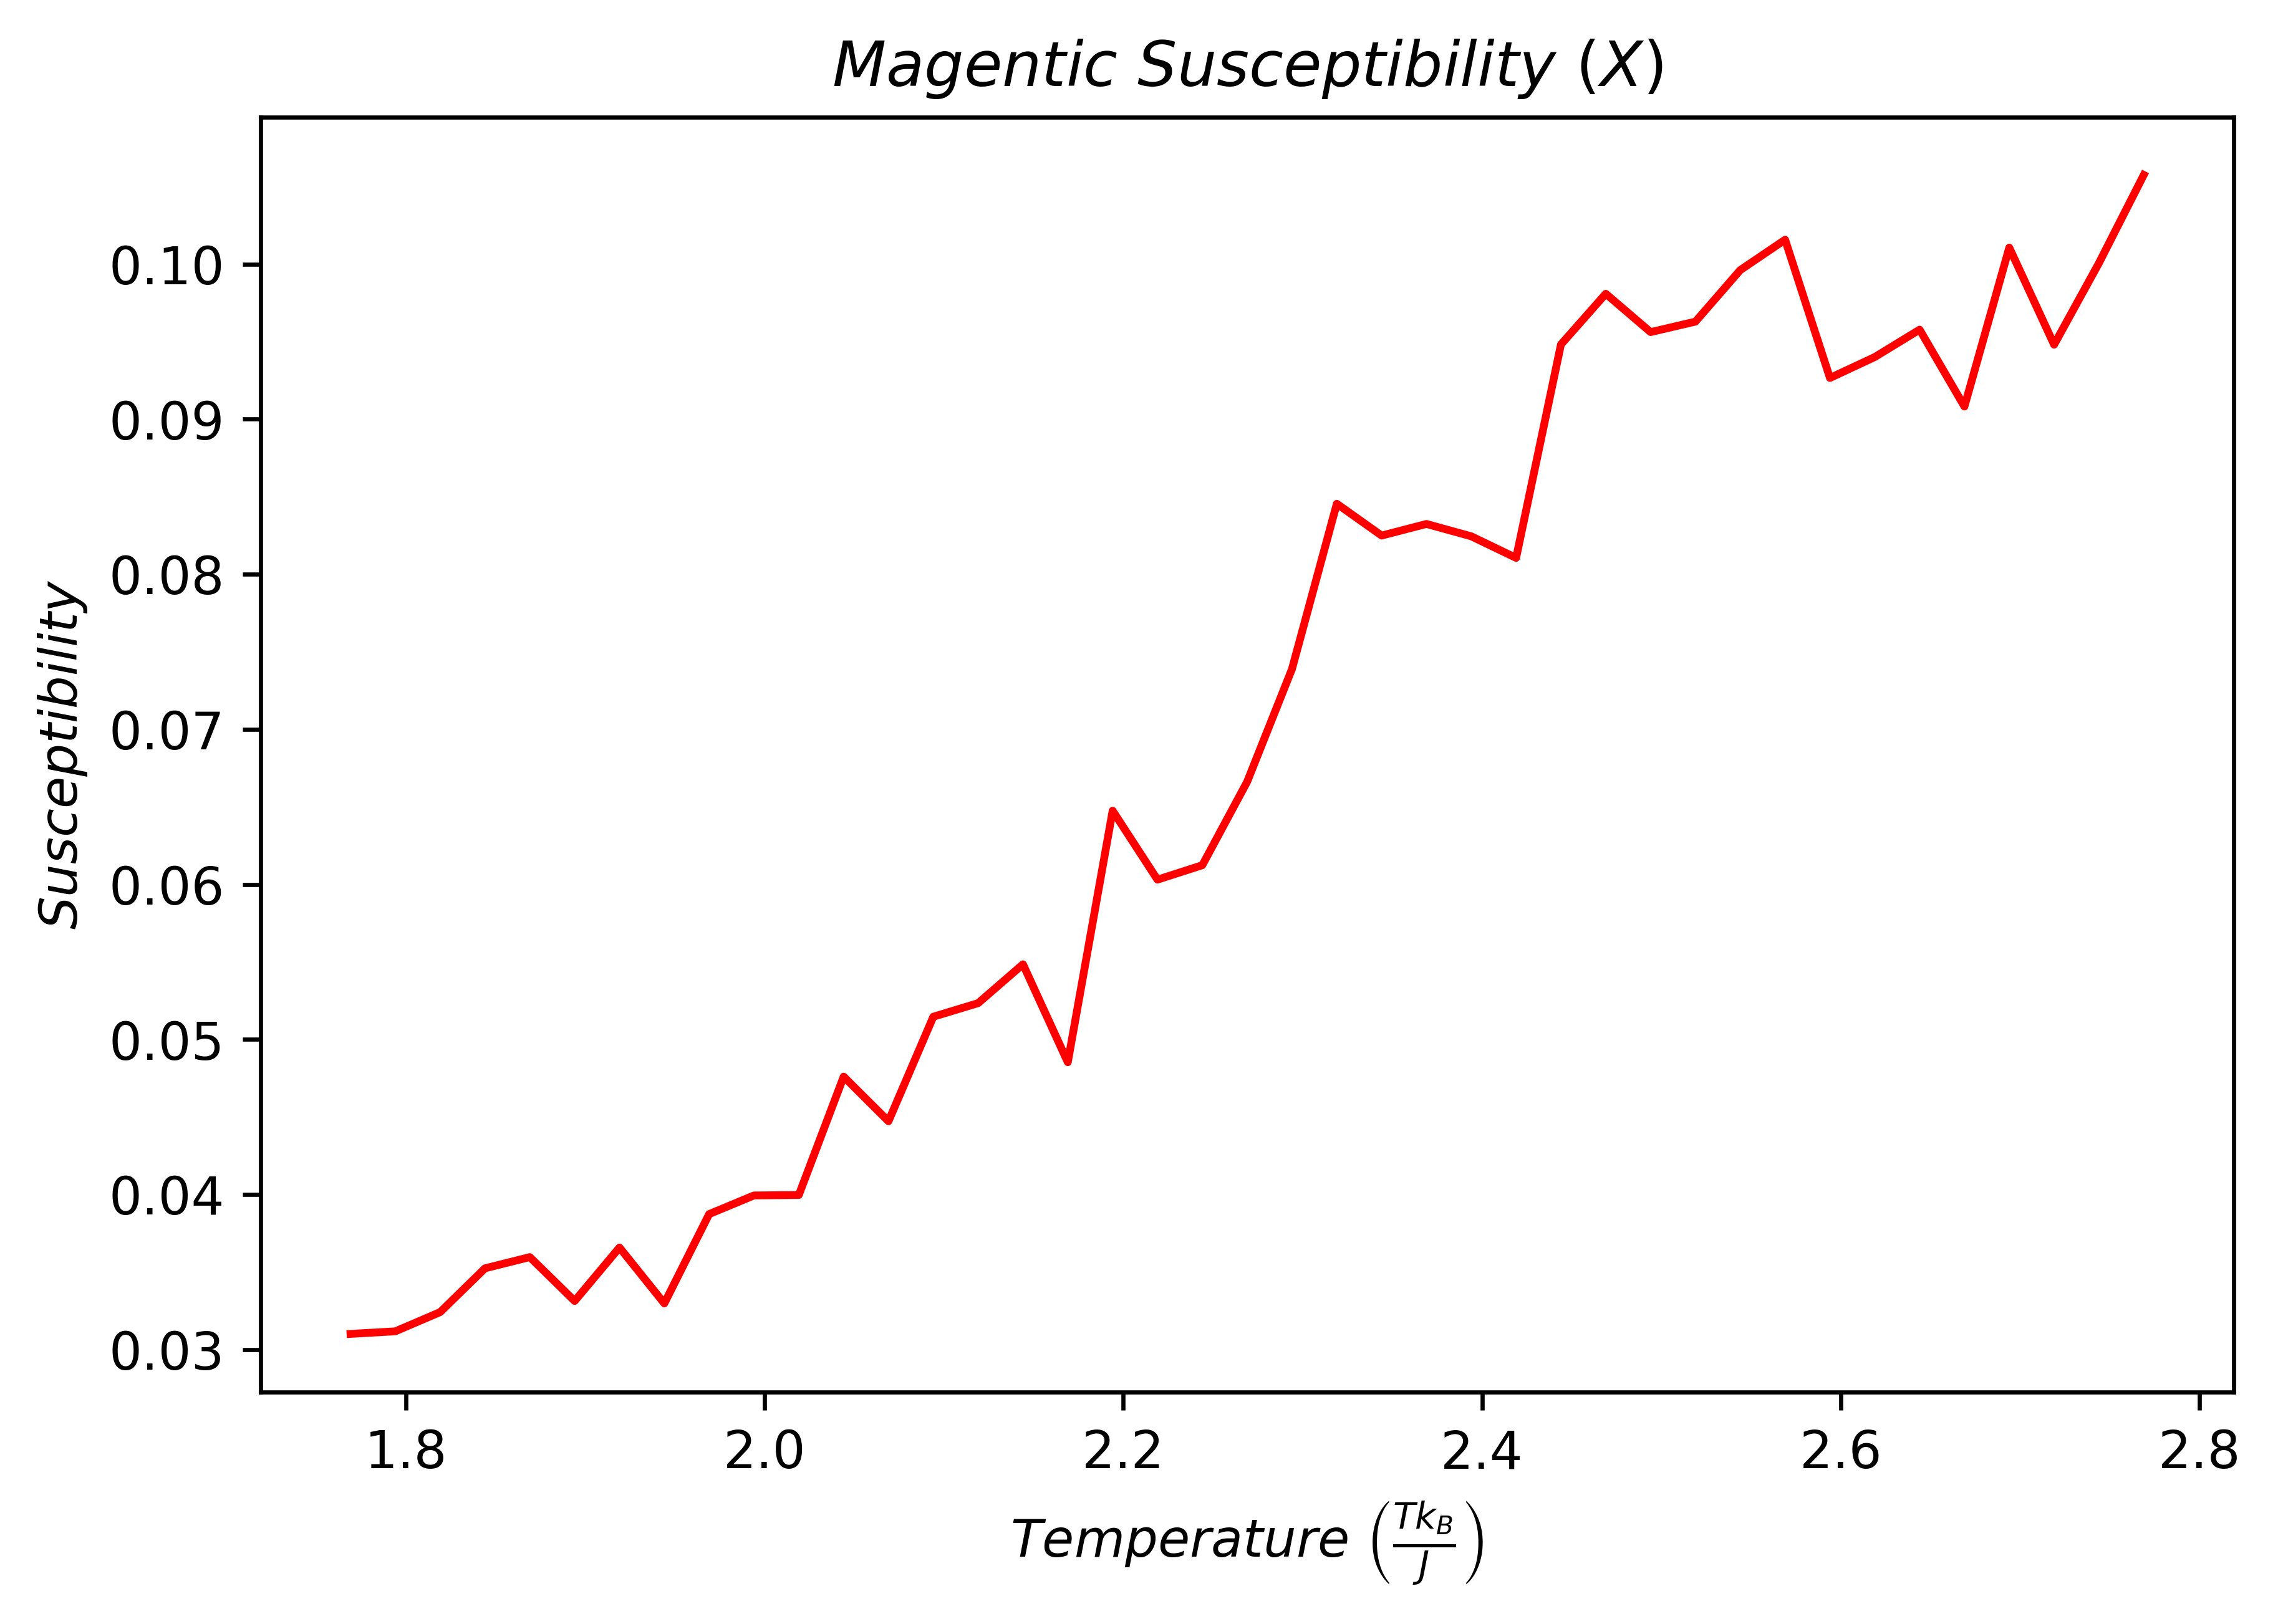
\includegraphics[scale=.45]{AntiMS128}
%\end{figure}
%\begin{figure}[h]
\caption{Mean Magnetization per dipole for the anti-ferromagnetic lattice. This plot shows that $\overline{m}$ fluctuates about zero.}
\centering
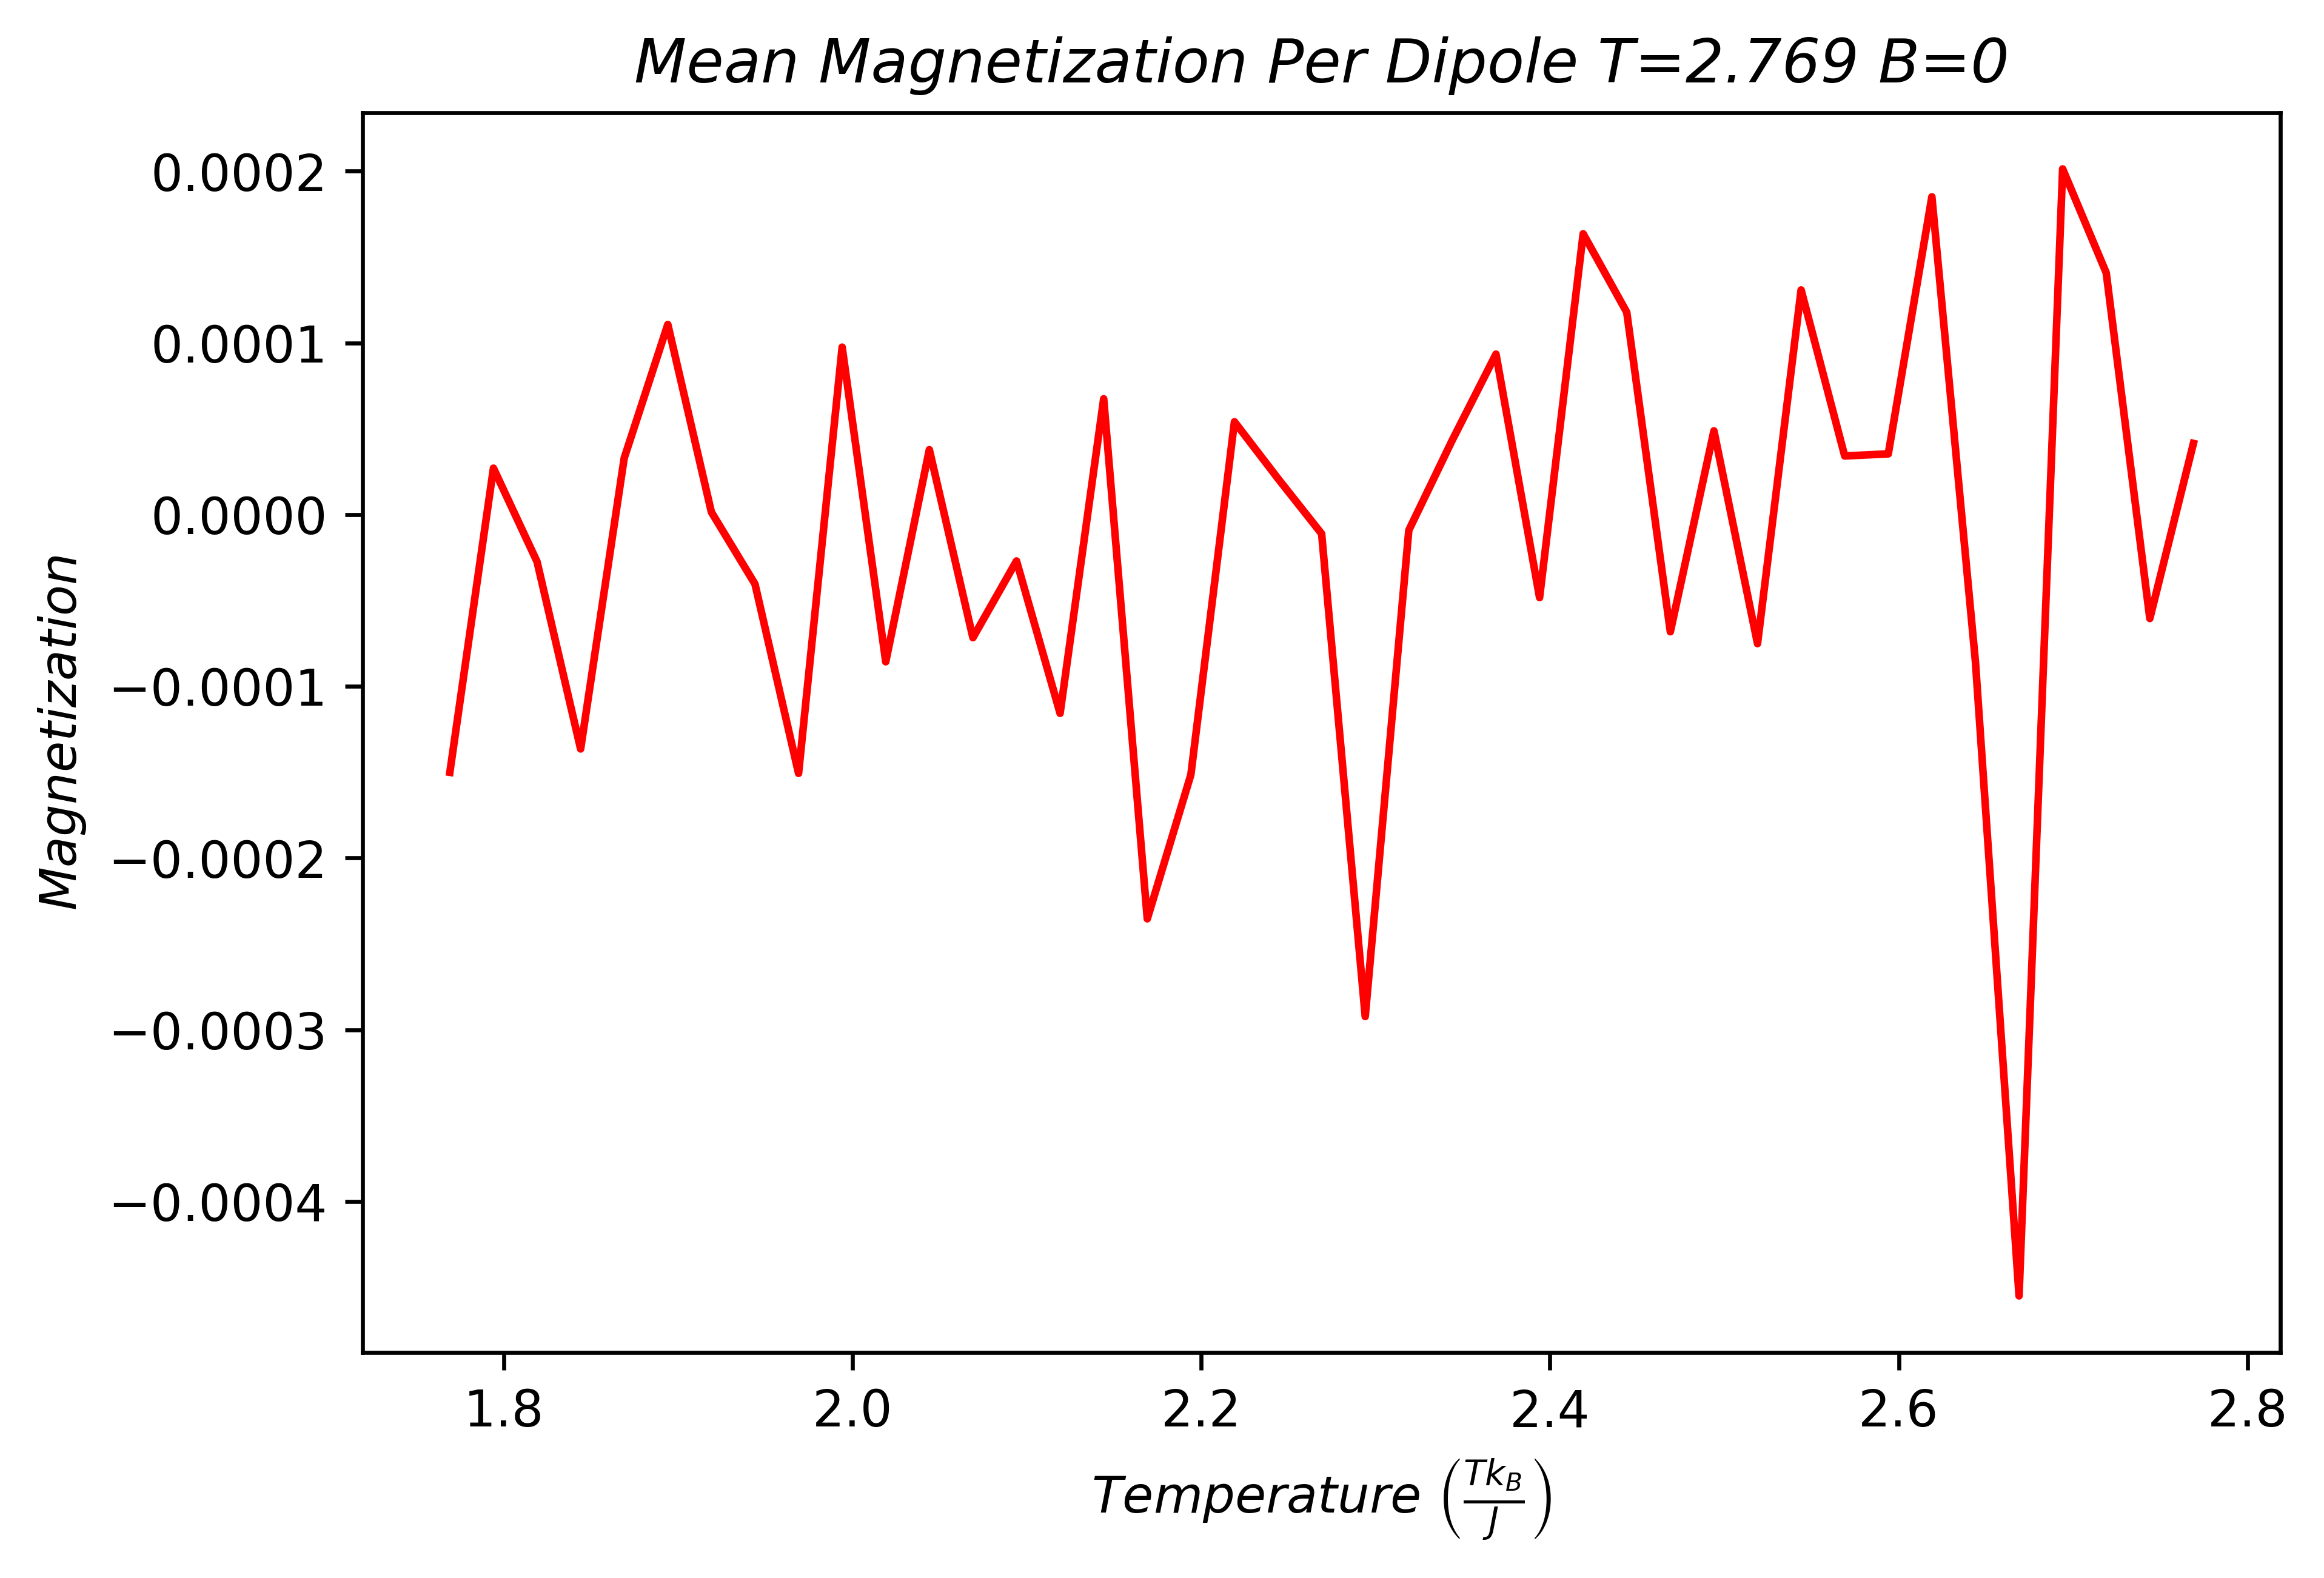
\includegraphics[scale=.45]{AntiMMT}
\end{figure}
\begin{figure}[H]
\caption{Specific Heat Capacity for the anti-ferromagnetic lattice. This plot reveals that the anti-ferromagnetic lattice still maintains a similar structure in its heat capacity.}
\centering
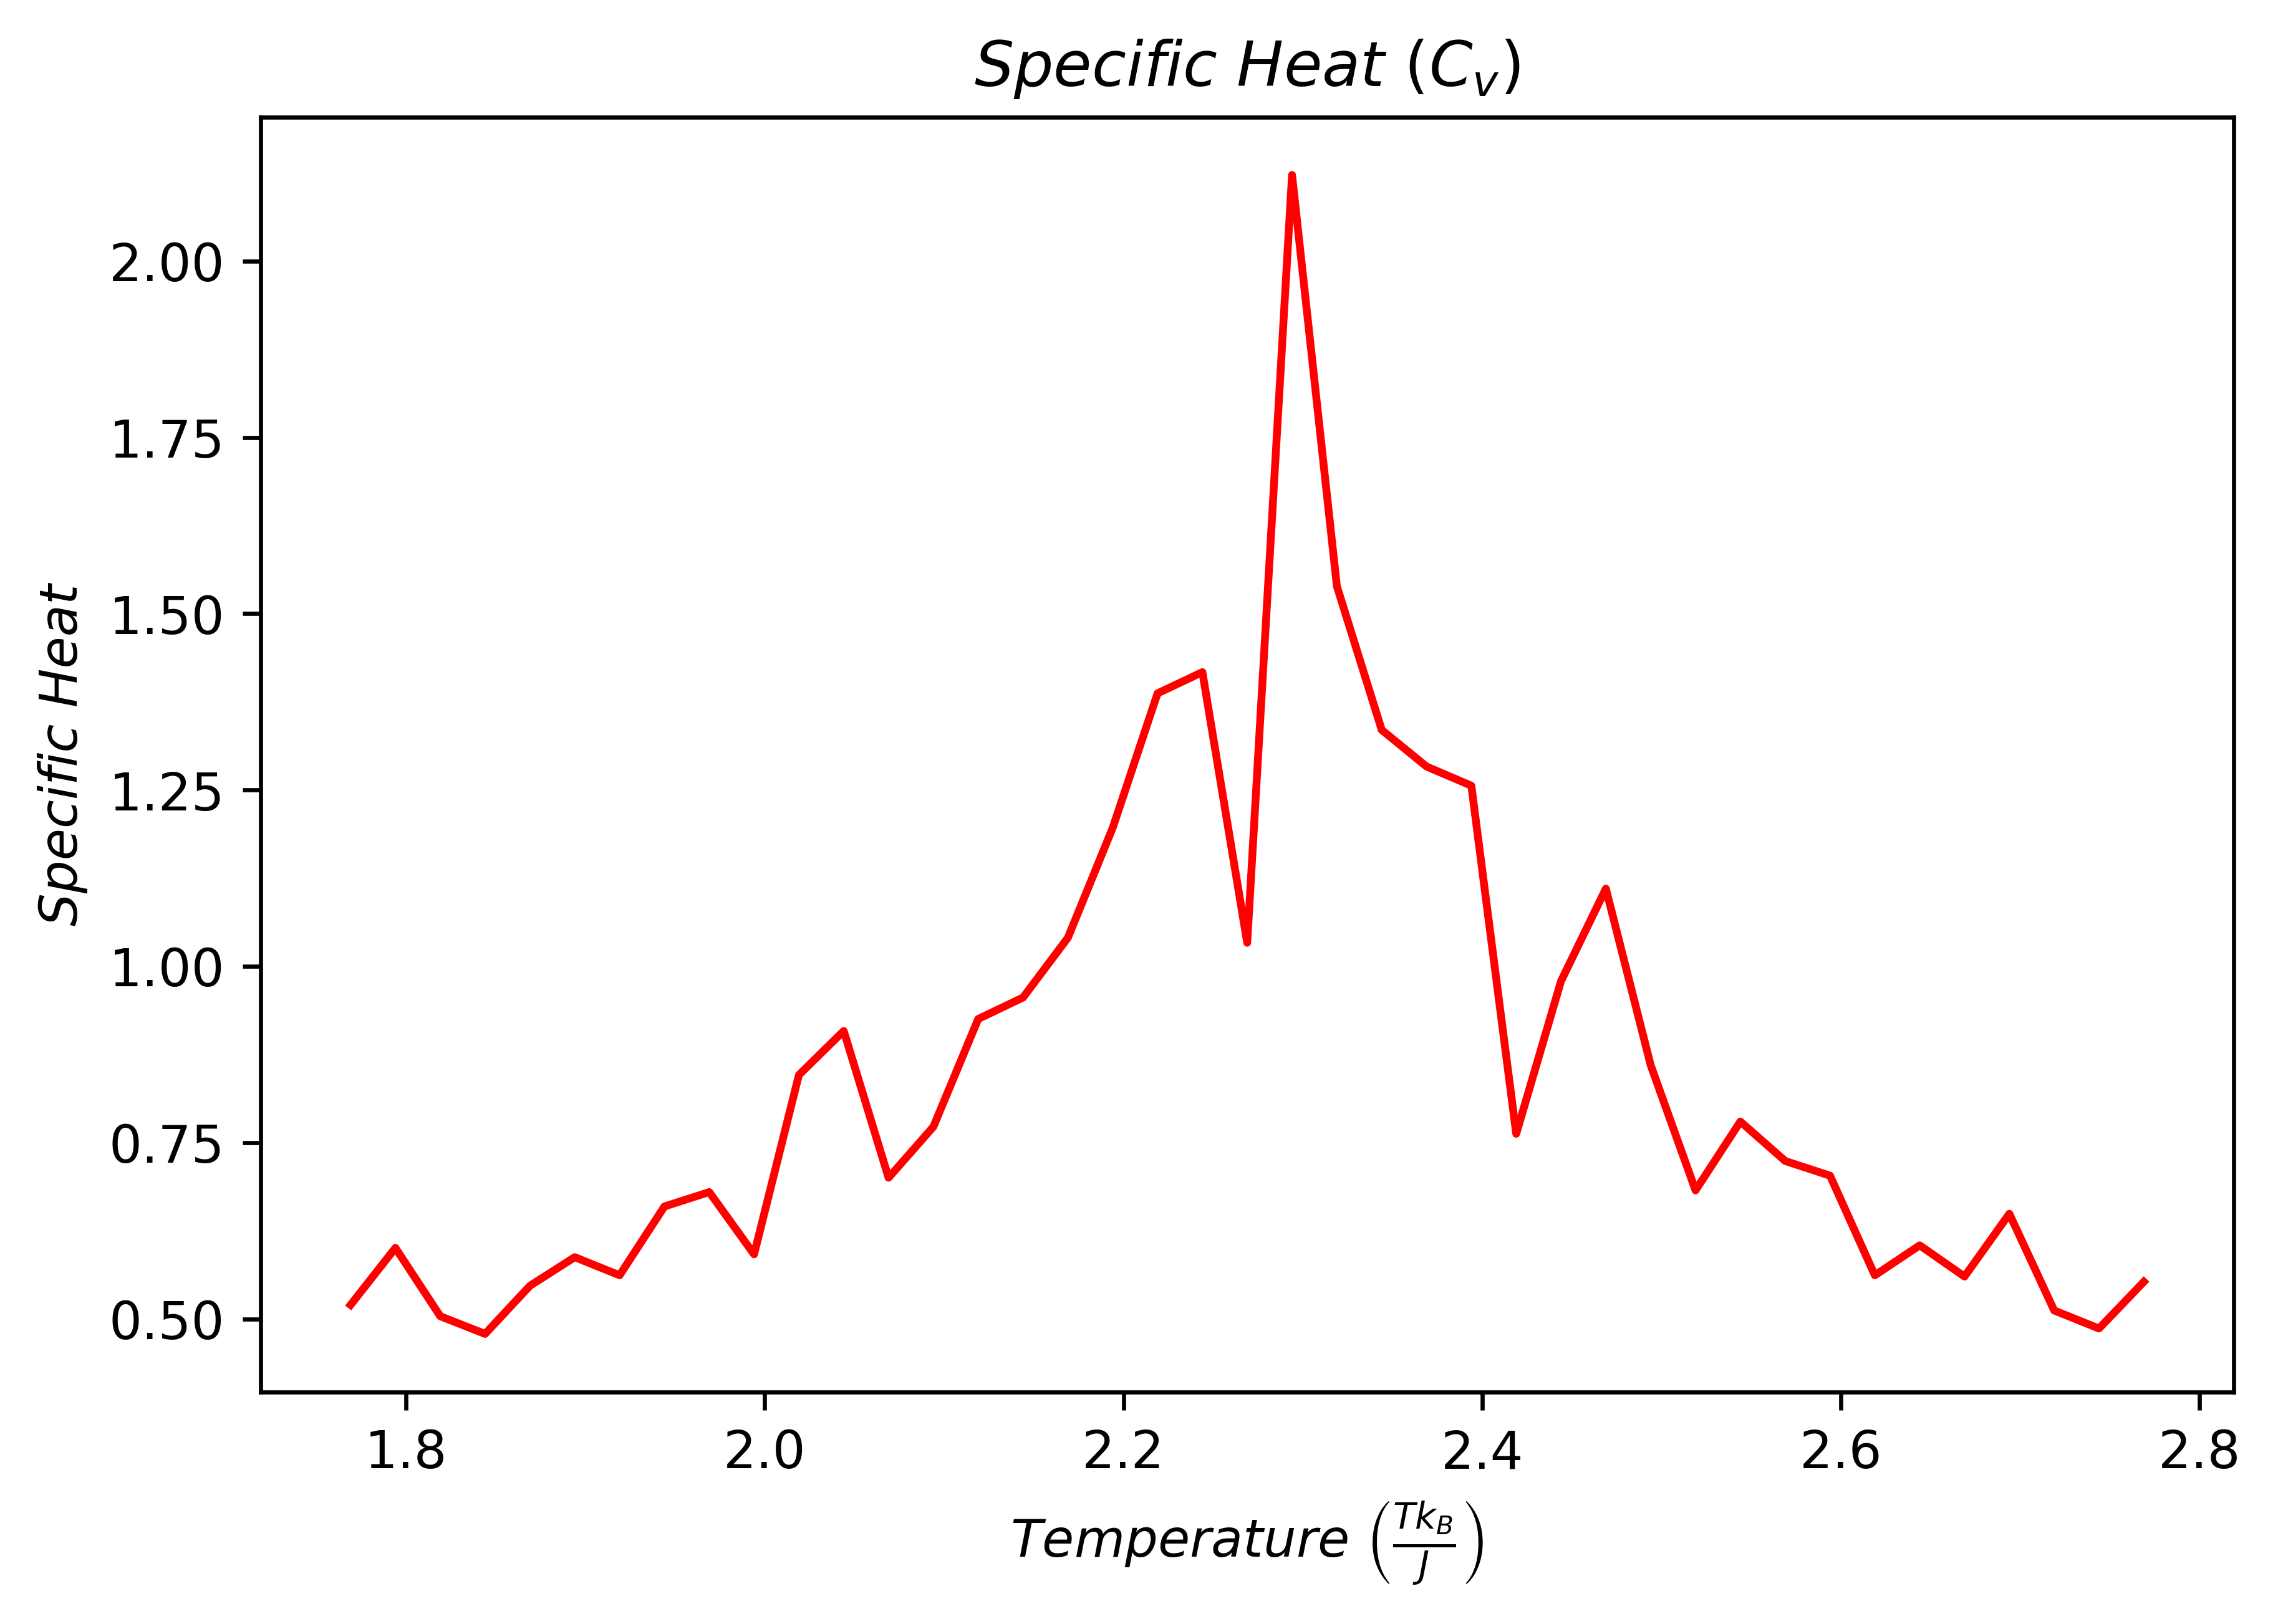
\includegraphics[scale=.45]{AntiSH128}
\end{figure}
%%%%%%%%%%%%%%%%%%%%%%%%%%%%%%%%%%%%%%%%%%%%%%%%%%%%%%%%%%%%
As a final note on this topic, it can be useful to see the structure of the lattice about the critical temperature to gain a better understanding of exactly how an anti-ferromagnetic Ising model operates - particularly about the phase transition. Hence, Figures (28), (29), and (30) show the structure of the lattice before the critical temperature, at the critical temperature, and after the critical temperature. In general, the structures are quite random and are similar to the ferromagnetic case when the temperature exceeds the critical temperature.
%%%%%%%%%%%%%%%%%%%%%%%%%%%%%%%%%%%%%%%%%%%%%%%%%%%%%%%%%%%%
\begin{figure}[H]
\caption{Anti-Ferromagnetic Lattice for $T=2.219<T_c$}
\centering
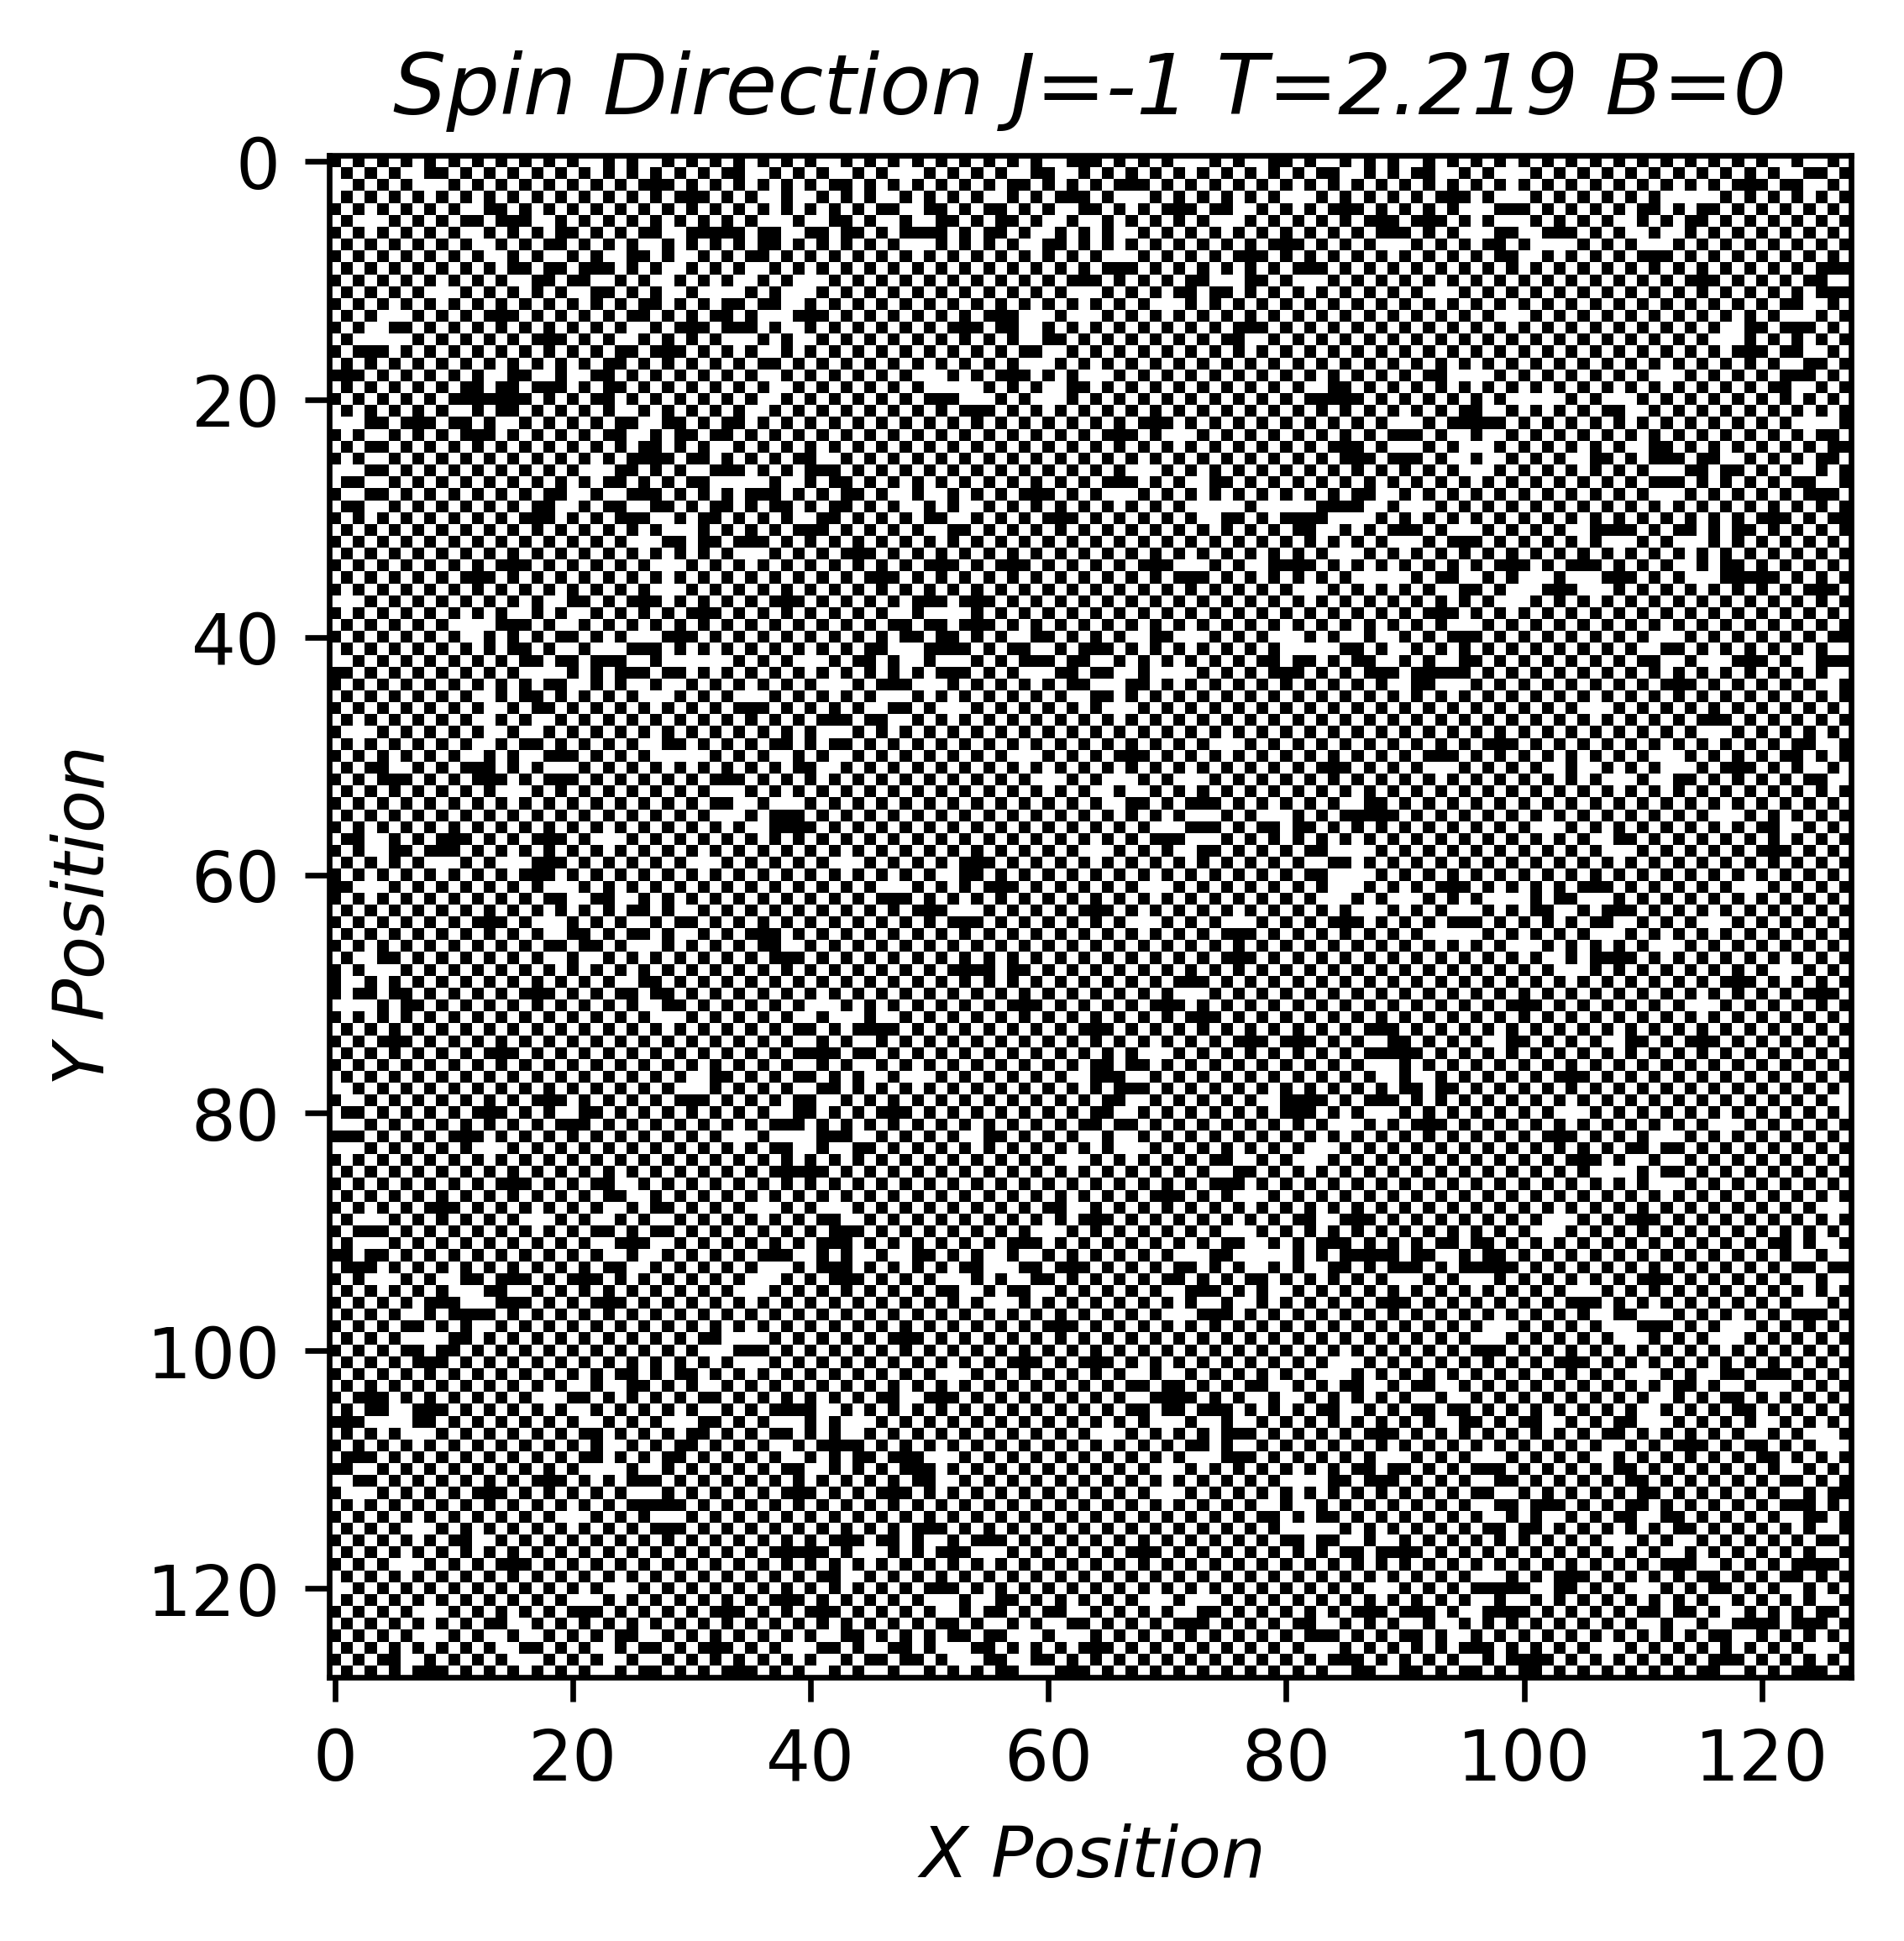
\includegraphics[scale=.55]{AntiFerro1T=2219}
%\end{figure}
%\begin{figure}[h]
\caption{Anti-Ferromagnetic Lattice for $T=2.269=T_c$}
\centering
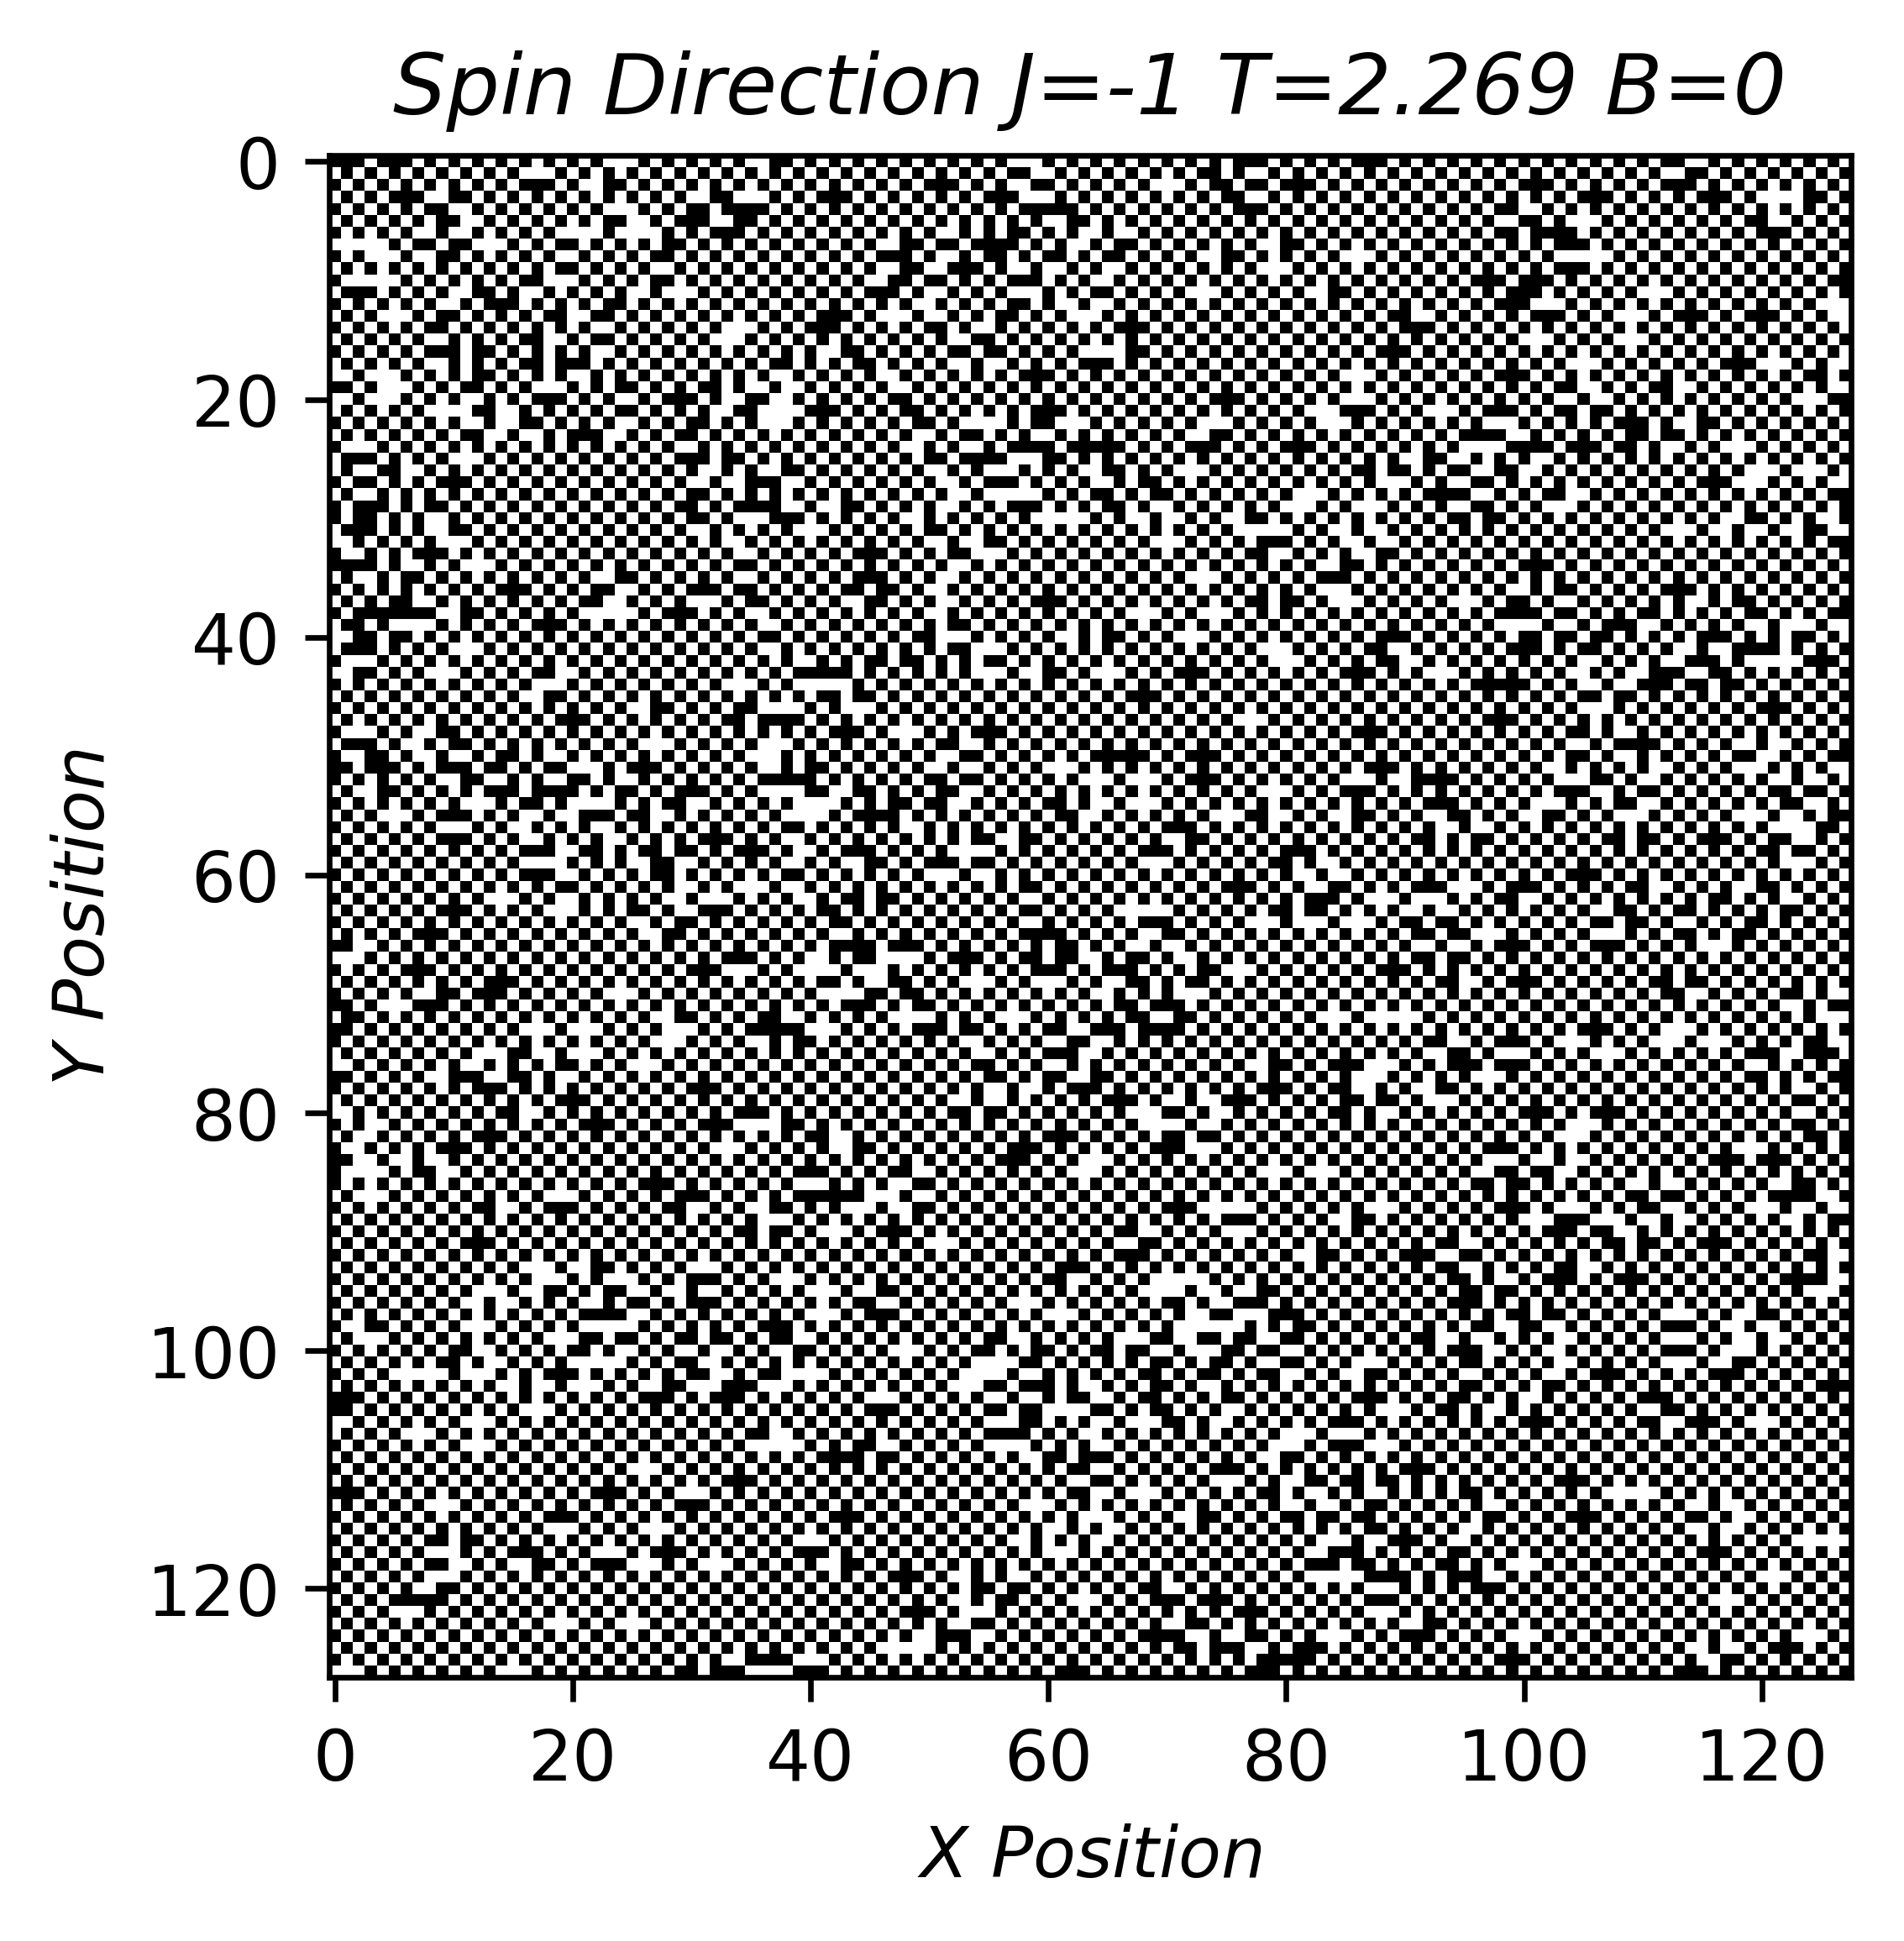
\includegraphics[scale=.55]{AntiFerro2T=2269}
%\end{figure}
%\begin{figure}[h]
\caption{Anti-Ferromagnetic Lattice for $T=2.294>T_c$}
\centering
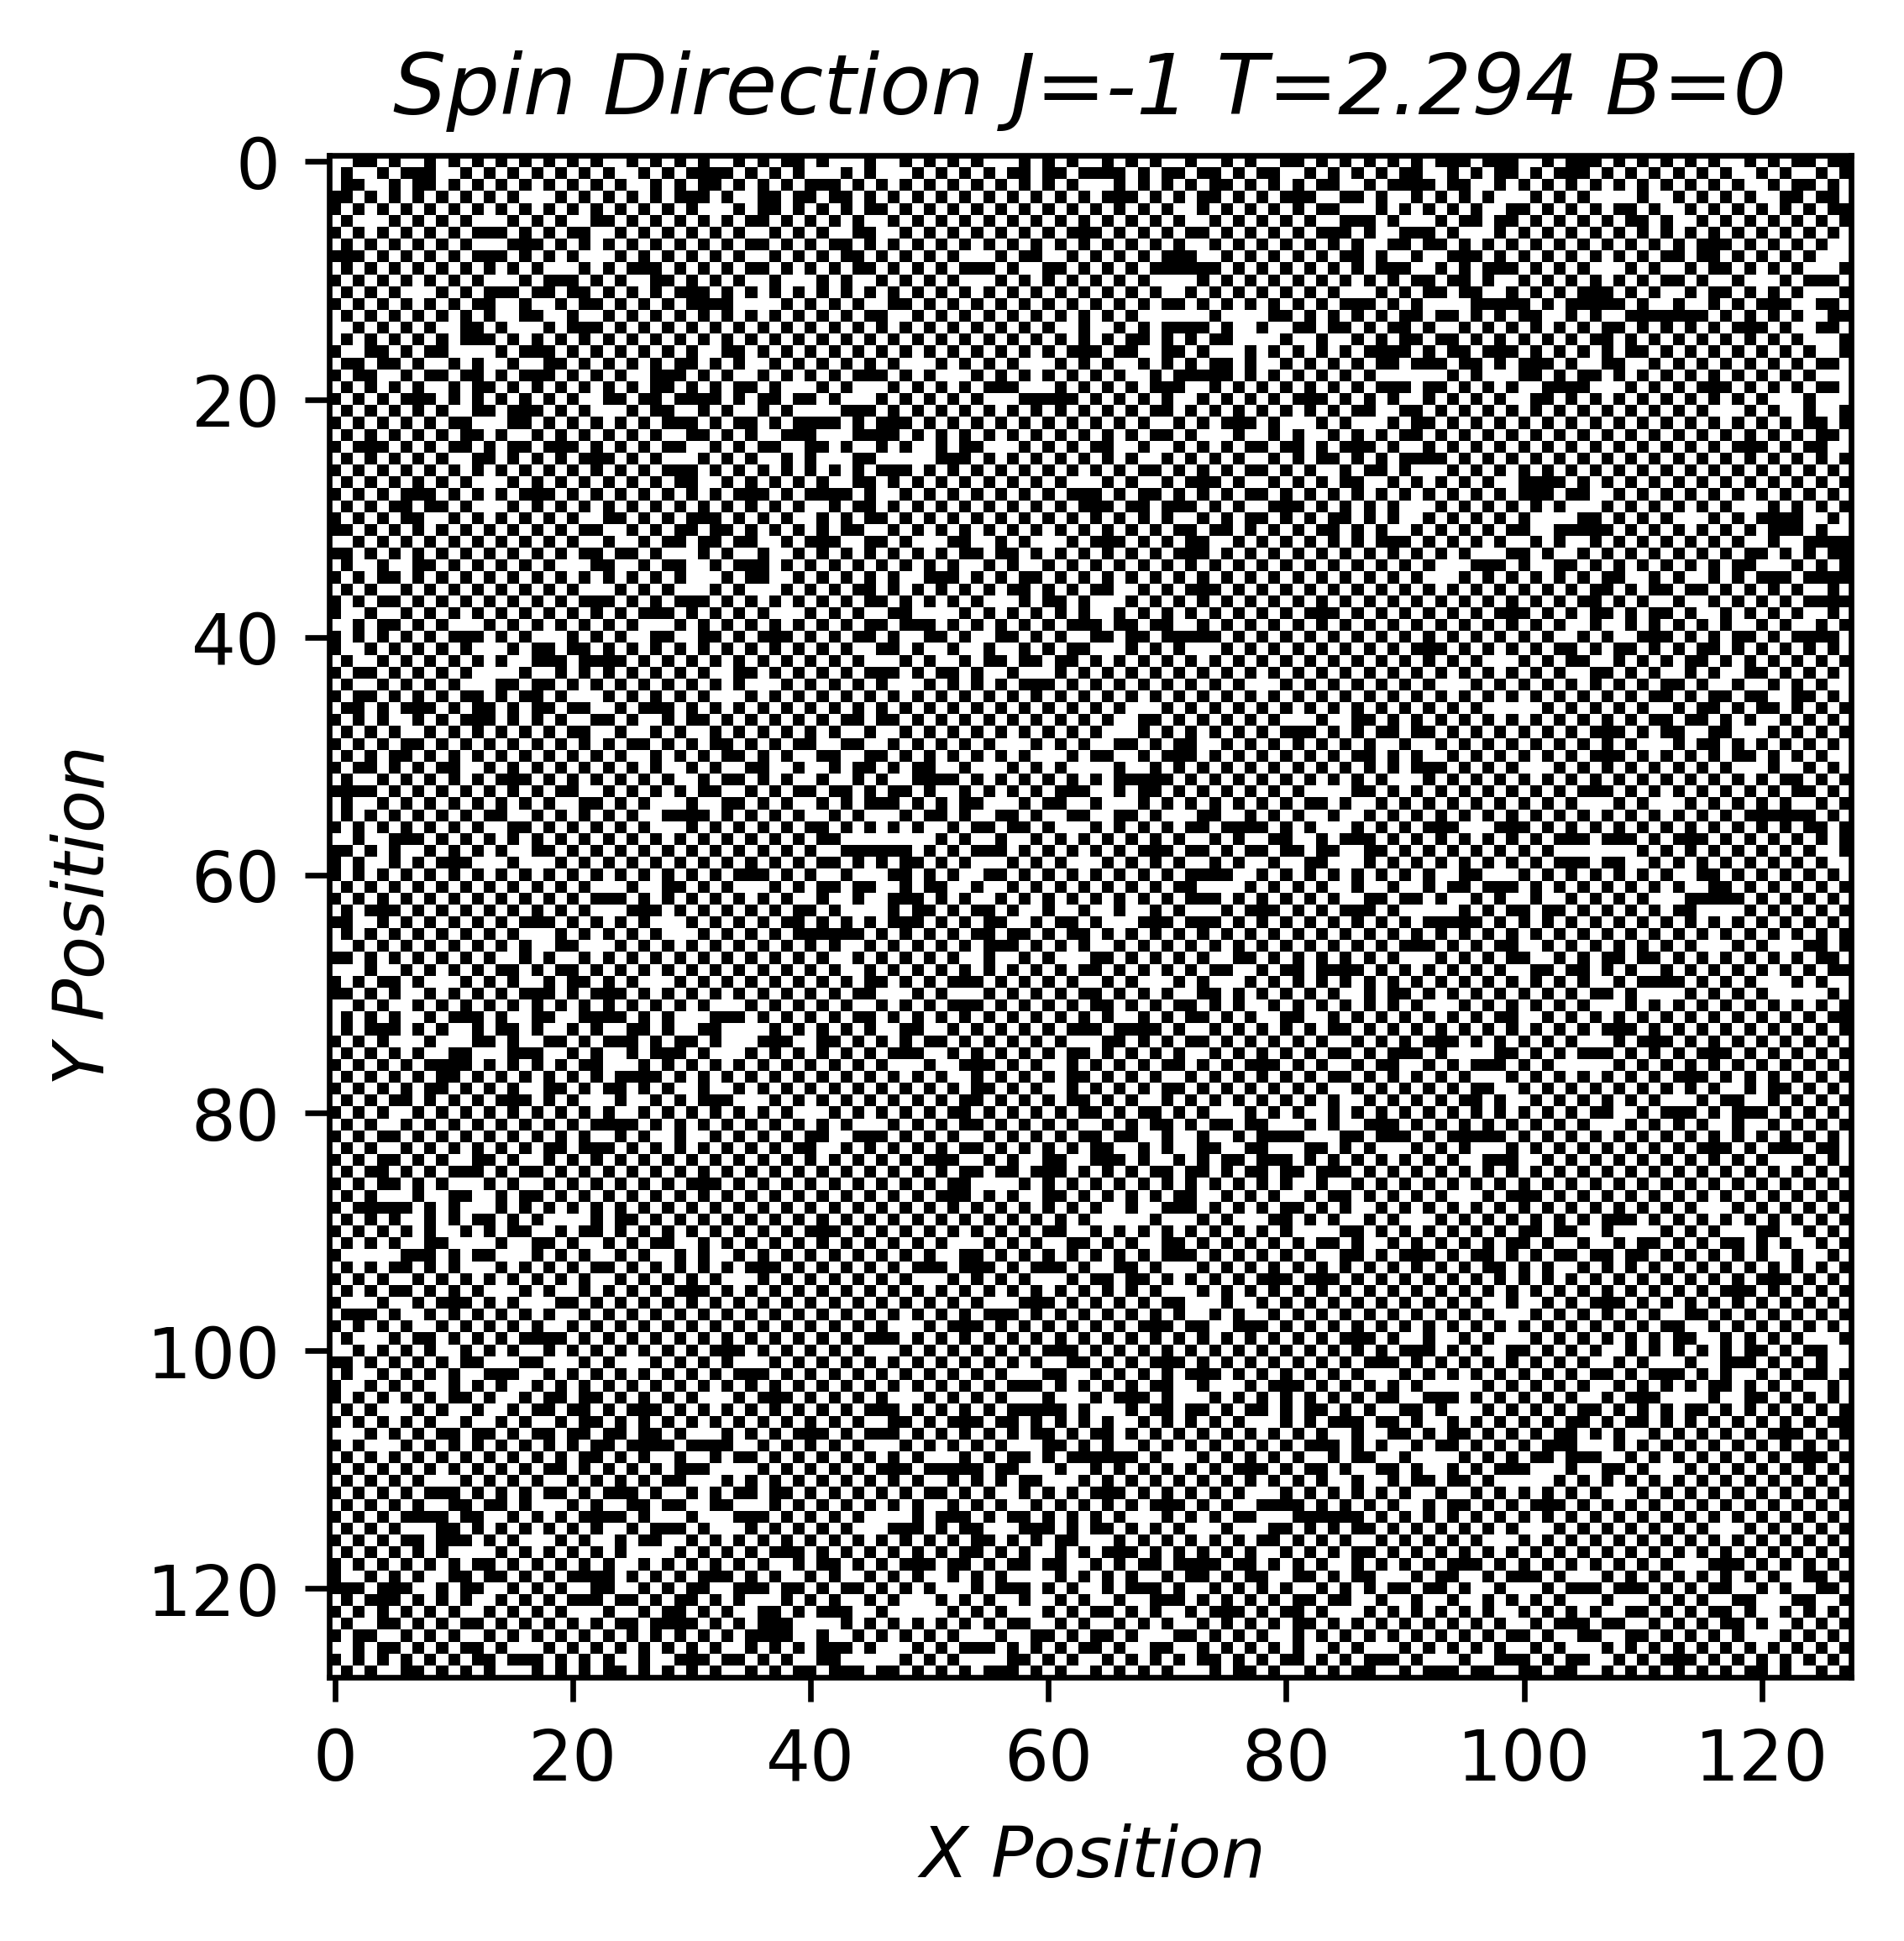
\includegraphics[scale=.55]{AntiFerro3T=2294}
\end{figure}
%%%%%%%%%%%%%%%%%%%%%%%%%%%%%%%%%%%%%%%%%%%%%%%%%%%%%%%%%%%%
%%%%%%%%%%%%%%%%%%%%%%%%%%%%%%%%%%%
% New Section
%%%%%%%%%%%%%%%%%%%%%%%%%%%%%%%%%%%
\section{Conclusion}
\hspace{\parindent} In conclusion, the first experiment successfully found the two phase changes that occur in $\overline{m}$ when the external heat bath was at a temperature that was less than the critical temperature. These two phase changes were shown to occur approximately at $B=-0.5$ and $B=0.5$, and that they formed a hysteresis as a result. When the external heat bath was at a temperature that was greater than the critical temperature, there was also shown to be no phase transitions in $\overline{m}$ because the "memory" of the lattice had been greatly reduced making it so the past compositions did not influence future compositions. Additionally, the first experiment successfully found that the number of independent samples in the auto-correlation function did depend on the magnetic field, and that the relationship between the temperature and magnetic field of the system greatly influenced the magnitude of the error bars of $\overline{m}$ as well. A greater magnetic field was shown to correspond with fewer samples and larger error bars, and a smaller magnetic field was shown to correspond with more samples and smaller error bars. In regards to the second experiment, it successfully determined that the amount of Monte-Carlo sweeps that needed to pass to adequately thermalize the lattice did depend on the external heat bath temperature. Temperatures under the critical temperature required more time (1750 sweeps in the case of $T=1$), where as temperatures at or above the critical temperature required much fewer (500 sweeps or less). When completely thermalized, the respective lattices of the different temperatures were also discerned to have entirely different structures: one alignment dominated in the $T \ll T_c$ case, small structures existed in the $T=T_c$ case, and utter randomness existed in the $T \gg T_c$ case. The second experiment additionally revealed that a second order phase transitioned occurred at the critical temperature. This was revealed by observing the specific heat capacity per dipole and the magnetic susceptibility per dipole as a function of temperature, where a strong peak occurred at the critical temperature and tapered out to the sides for both plots. This structure indicated that a divergence was attempting to occur if not occurring outright which is a tell tale sign of a second order phase transition. The final experiment successfully portrayed the nature of the anti-ferromagnetic Ising model by changing the exchange coupling value from 1 to -1, thereby altering the system entirely. Interestingly, this model displayed a nearly identical specific heat capacity plot to the ferromagnetic plot, despite having completely different magnetic susceptibility plot and mean magnetization per dipole plot. This was somewhat expected, however, because a continuous phase transition between antiferromagnetism-paramagnetism is known to occur at the Neel temperature of $T_N=T_c=2.269$, hence, at the very least the specific heat capacity plot had to look remotely similar. Overall then, the experiments were highly successful and well predicted - with what errors that may have occurred being discussed at length. 
%%%%%%%%%%%%%%%%%%%%%%%%%%%%%%%%%%%
% New Section
%%%%%%%%%%%%%%%%%%%%%%%%%%%%%%%%%%%
\begin{thebibliography}{9}
\bibitem{latexcompanion} 
Wei Cai
\textit{A Introduction to Statistical Mechanics}.
(2011)
\bibitem{latexcompanion} 
I. Vattulainen, T. Ala-Nissila, and K. Kankaala
\textit{Physical tests for random numbers in simulations,}. 
(1994).
\bibitem{latexcompanion} 
D. P. Landau, S.-H. Tsai, and M. Exler,
\textit{A new approach to Monte Carlo simulations in
statistical physics: Wang-Landau sampling}. 
(2004).
\end{thebibliography}
\end{document}